The Compact Muon Solenoid (CMS) detector operates at the LHC at CERN. It was designed to operate in proton-proton (and lead-lead)
collisions at a center-of-mass energy of 14\TeV (5.5\TeV) and at
luminosities up to 10$^{34}$cm$^{-2}$s$^{-1}$
(10$^{27}$cm$^{-2}$s$^{-1}$). The CMS has cilindrical geometry and
its dimensions are a length of 21.5 m, a diameter of 14.6, and a total
weight of 12,500 tons. At the heart of the CMS detector system
lies a 4\unit{T} magnetic field produced by a large-bore superconducting
solenoid which encloses a silicon -- pixel and strips -- tracker, a homogeneous
lead-tungstate crystal electromagnetic calorimeter, and a brass-scintillator
sampling hadron calorimeter. Outside the superconducting solenoid lies
an iron yoke for magnetic flux-return instrumented with four stations
for muon detection. Forward sampling calorimeters extend the rapidity
coverage up to $\eta < 5$ and thus ensure good
hemiticity. Figure~\ref{fig:cmsDetector} shows an schematic representation
of the CMS detector and Figure~\ref{fig:cmsSlice} shows a cartoon
with a cross-sectional-slice view of the CMS detector along with
different particle detections.
\begin{figure}
 \centering
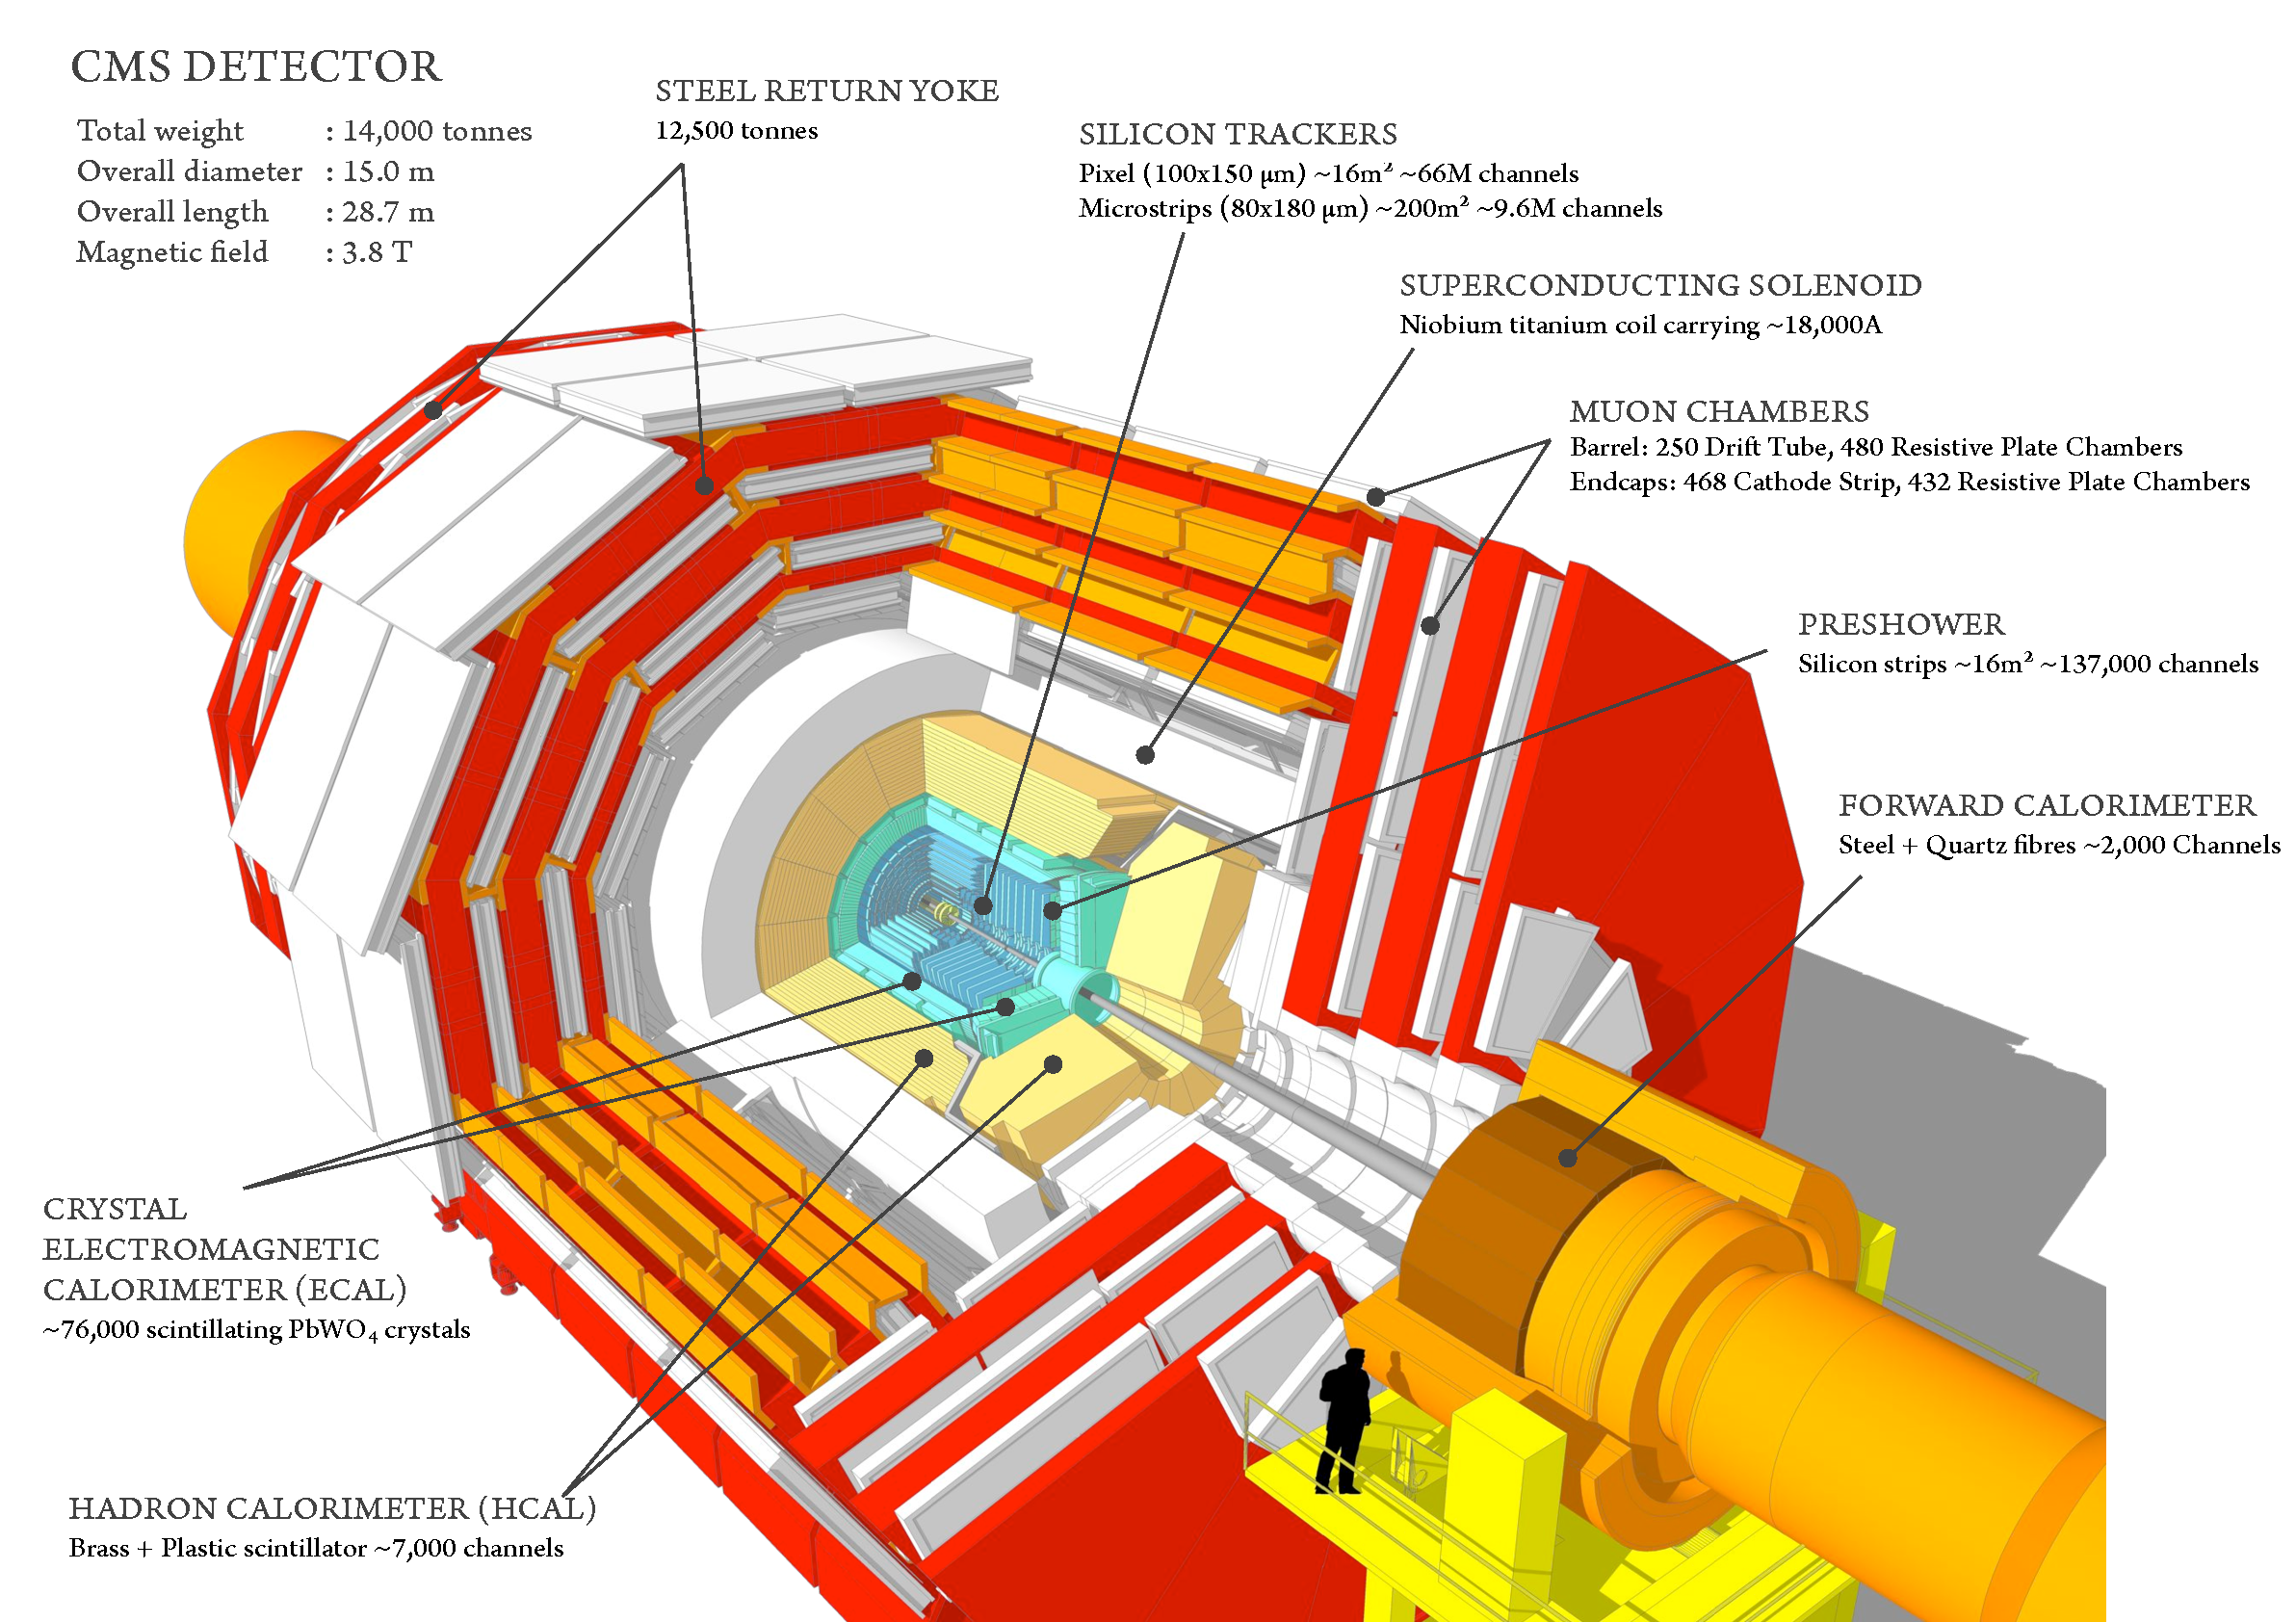
\includegraphics[width=0.99\textwidth]{CMS_DetectorFigures/cms_detector.png}
 \caption{A perspective view of the CMS detector.\label{fig:cmsDetector}}
\end{figure}
\begin{figure}
 \centering
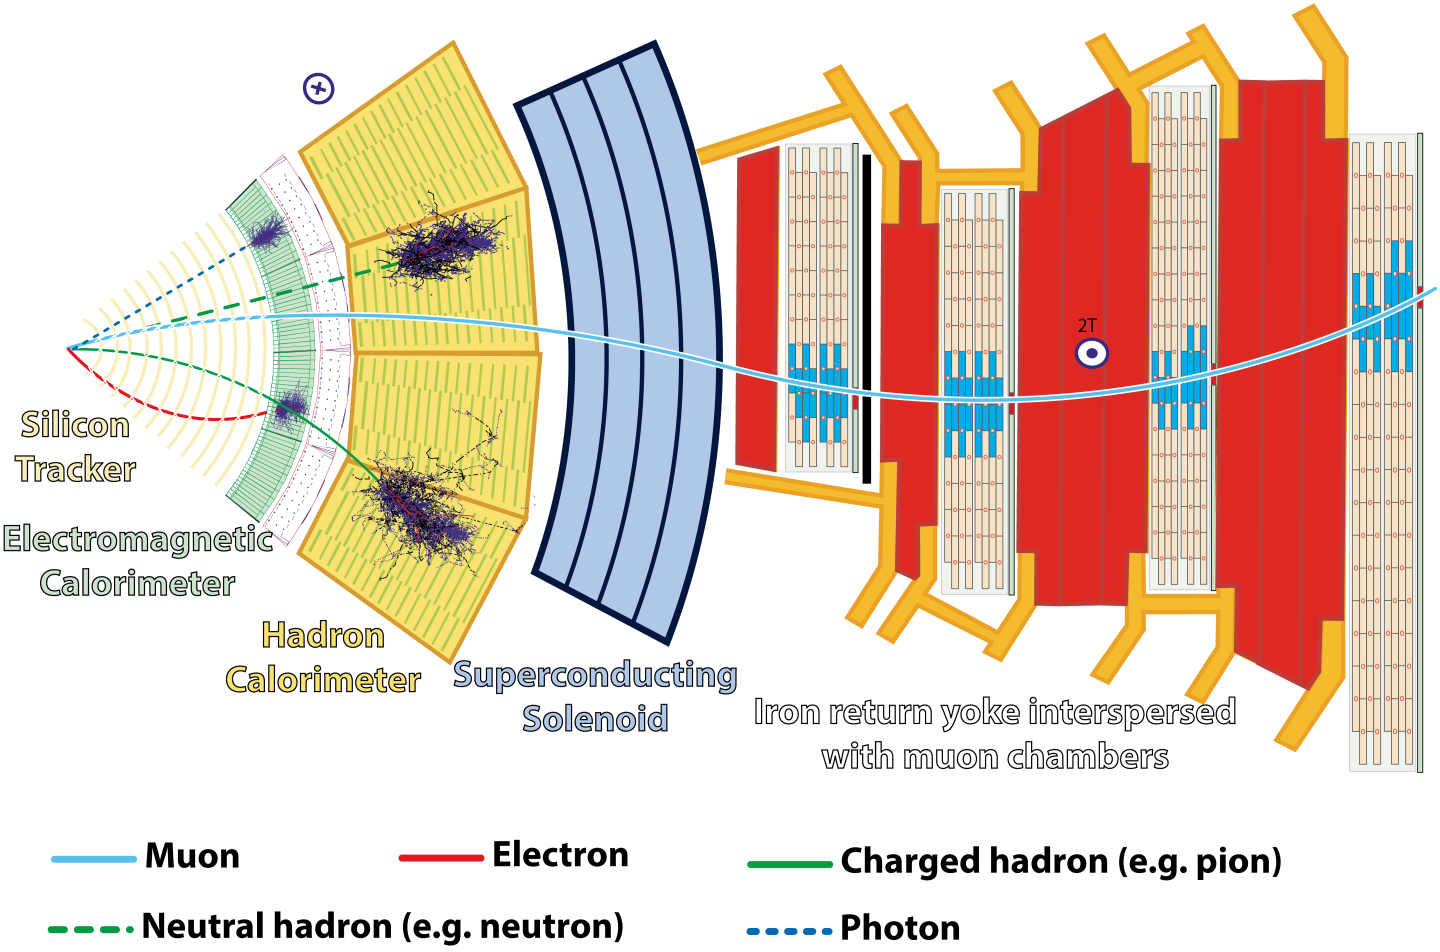
\includegraphics[width=0.99\textwidth]{CMS_DetectorFigures/CMSslice.png}
 \caption{A cross-sectional-slice view of the CMS detector. The
   different components of the detector are clearly labeled and
   different particle detections are depicted.\label{fig:cmsSlice}}
\end{figure}

This chapter presents an introduction to the CMS detector systems and
reconstruction algorithms. It is by no means a complete picture of the
CMS detector and its mostly based on Ref.~\cite{Chatrchyan:2008zzk}.
\section{The Tracker System}
The tracker is the innermost system of the CMS detector.
It was designed to measure efficiently and precisely the trajectories
of charged particles coming from the interaction points, as well as to
provide a precise reconstruction of the secondary vertices at each
bunch crossing. When running at the LHC designed conditions, every
buch crossing, i.e 25 ns, the number of proton-proton collision will
be about 20 and they will produce an average number of particles of about
1000. These conditions and the above requirements implied a highly granular and fast
response design. That being said, this design due to its high power
consumption requires an efficient cooling system which in turn is in
conflict with the goal of minimizing the material budget and thus
reduce unwanted interactions. In addition, the harsh radiation
environment that will deteriorate the detector performance posed
further challenges in its construction. Therefore, the system --
silicon sensors, readout, mechanical structures, granularity, etc --
was designed to operate for 10 year and satisfying the considerations
listed above. The CMS tracker is composed of three layers of pixels
detectors up to a radius of 10.2 cm, a 10-layer silicon strip tracker
up to a radious of 1.1 m, two endcap disks at each side of the barrel pixel detectors, 3
endcap disks at each side of the inner region of the strips (up to a
radius of 55 cm), and finally 9 disks covering the $|z|$ > 120 cm
regions starting a radious of 55 cm. More details about the tracker
layout will be given below and are summarized in
Figure~\ref{fig:trackerlayout}. The tracker covers up to
pseudorapidities of $|eta| < 2.5$ with a about 200 m$^2$ of active
silicon area implemented. The material budget of the CMS tracker is
shown in Figure~\ref{fig:materialBudget}. As it can be seen the most
heavily implemented pseudorapidity is found to be at $|\eta|\approx$ 1.4.
\begin{figure}
 \centering
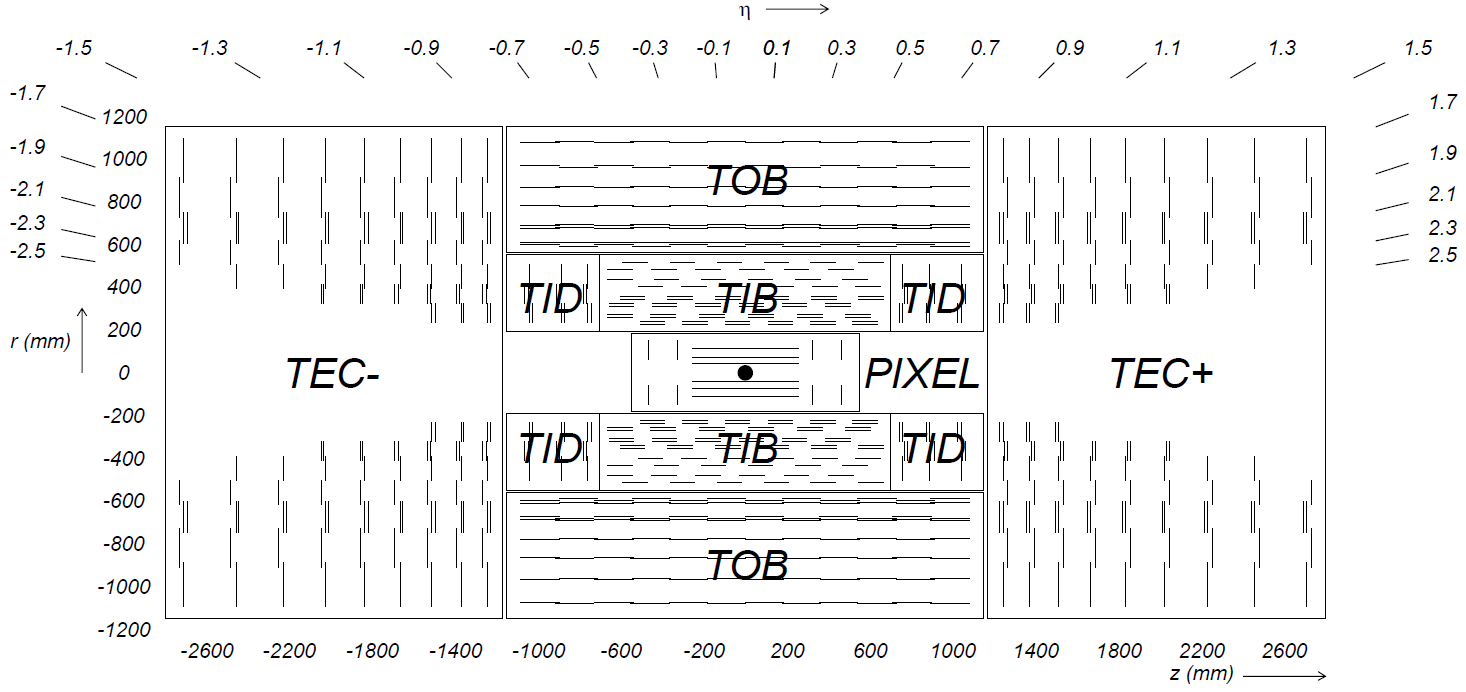
\includegraphics[width=0.99\textwidth]{CMS_DetectorFigures/TrackerLayout.png}
 \caption{A cross-sectional view of the silicon tracker layout. The
   different subsytems are clearly labeled.\label{fig:trackerlayout}}
\end{figure}
\begin{figure}
 \centering
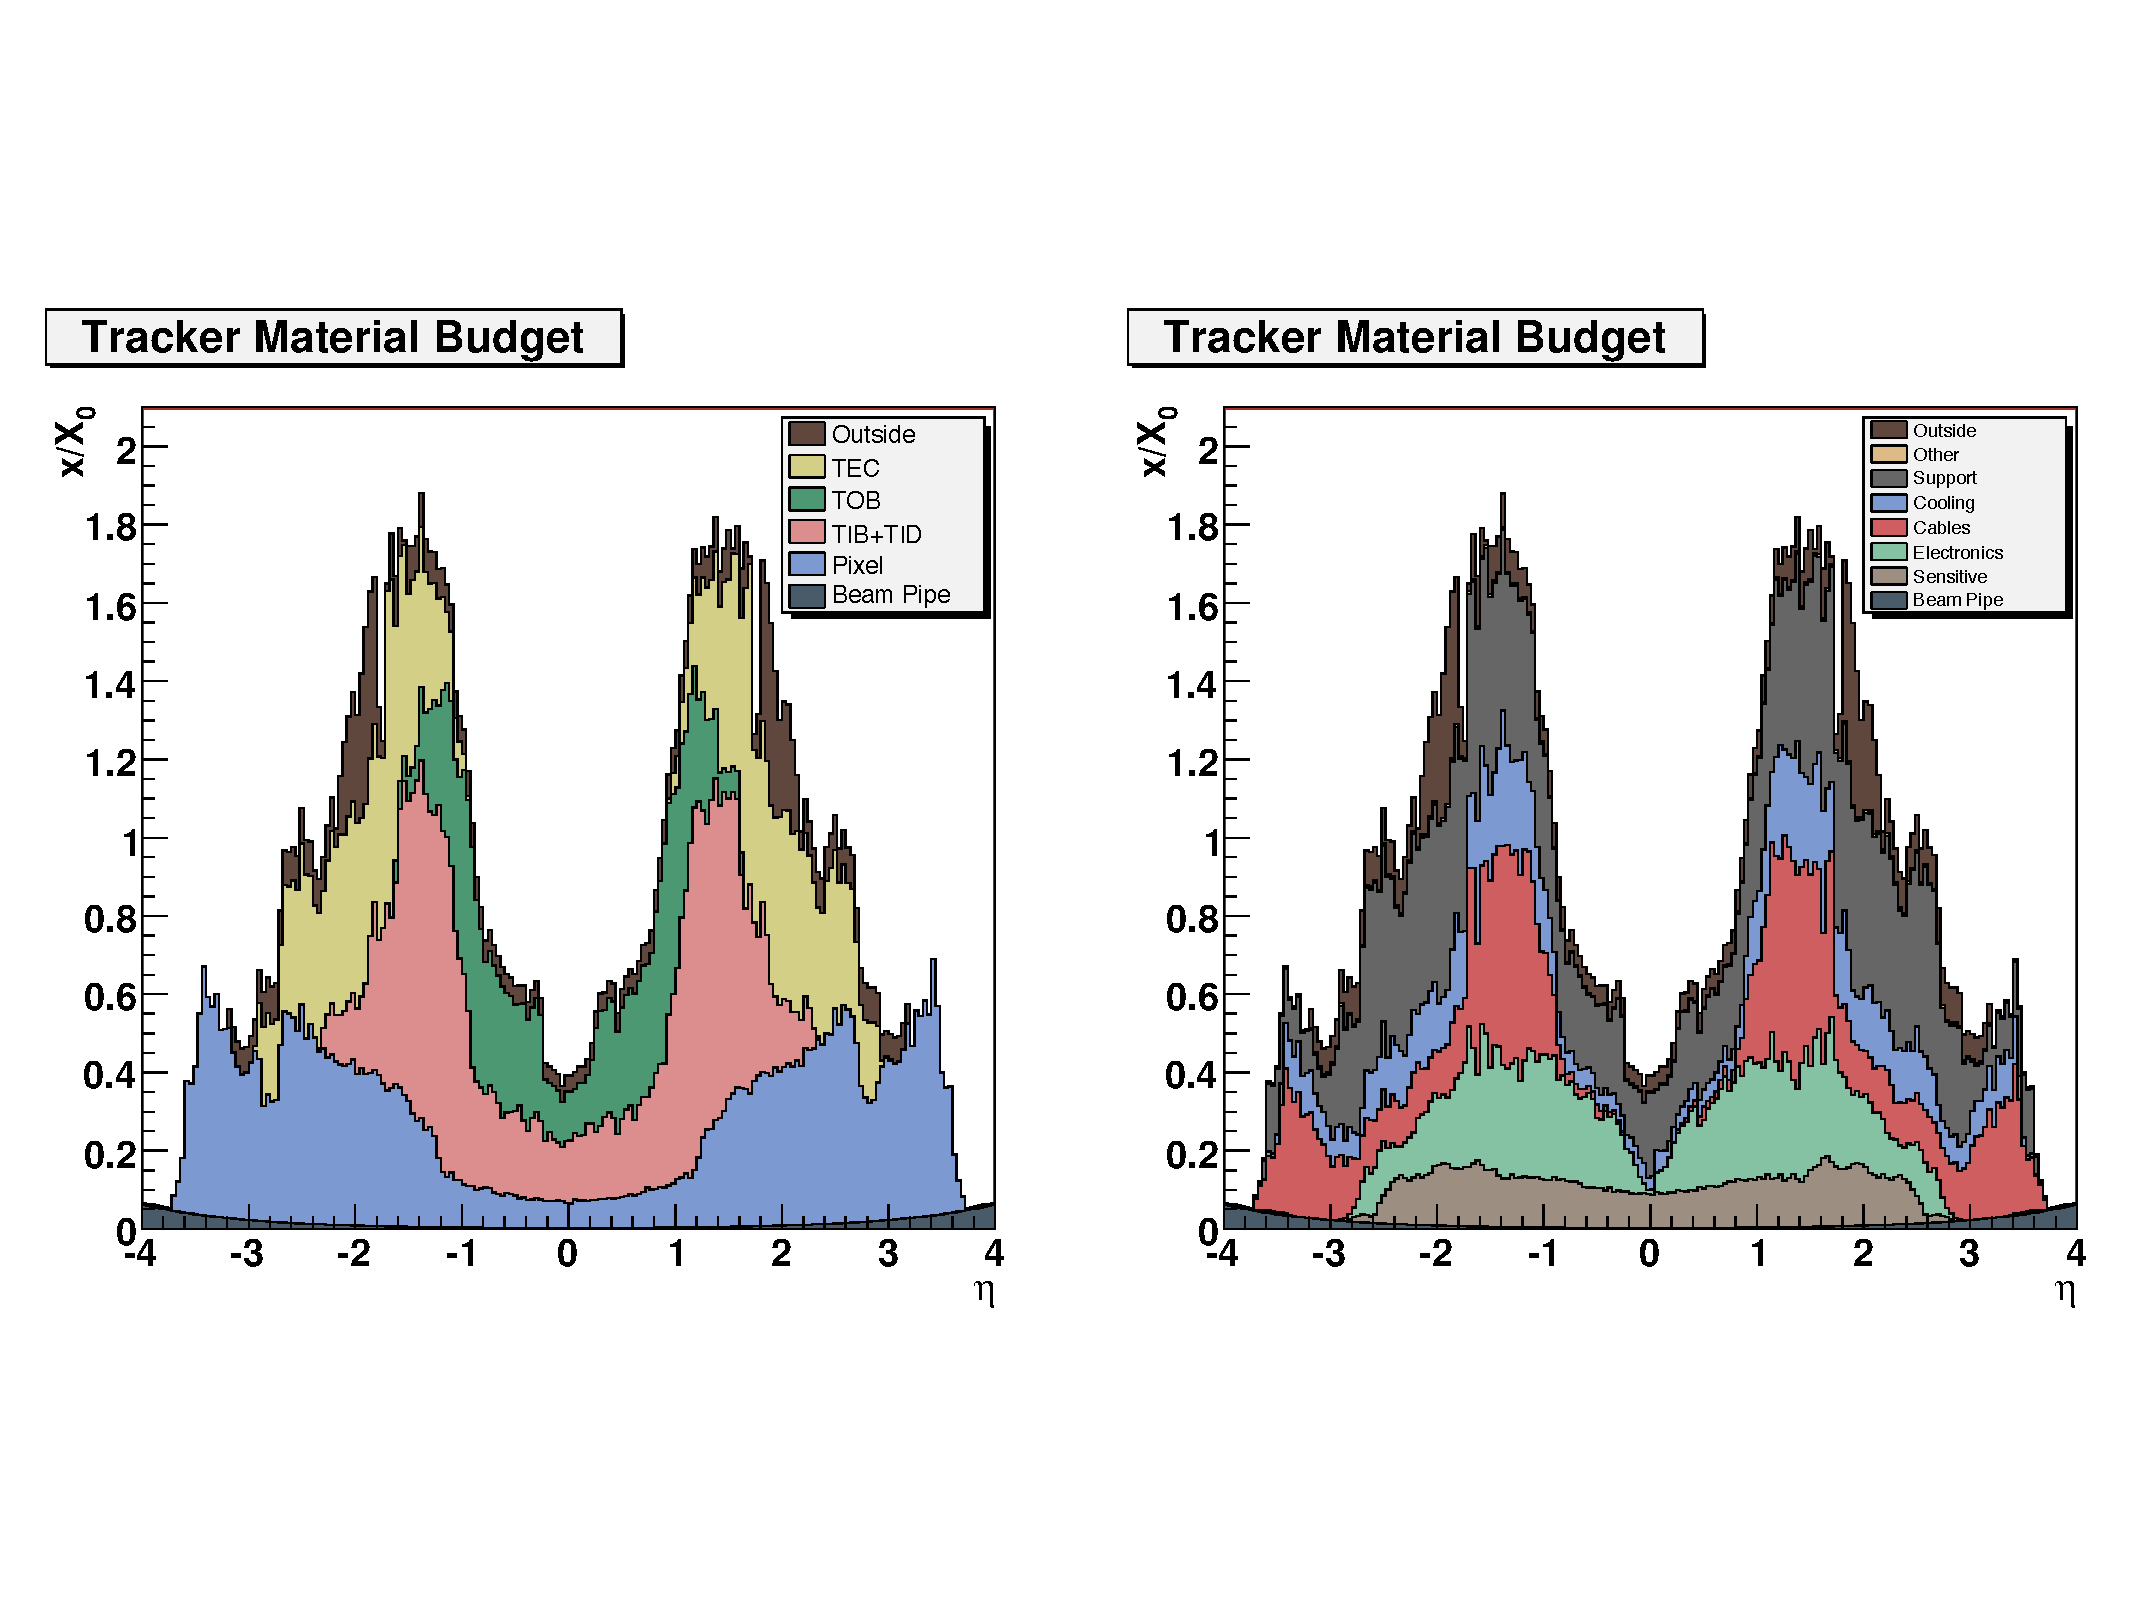
\includegraphics[width=0.99\textwidth]{CMS_DetectorFigures/TrackerMaterialBudget.pdf}
 \caption{Material budget of the CMS tracker in units of radiation
   length as a function of pseudorapidity $\eta$ for the (left)
   different subdetectors and (right) functional contributions.\label{fig:materialBudget}}
\end{figure}
\subsection{Pixel Tracker}
The inner pixel detector is composed of three 53-cm-long cylindrical layers at a
radii of 4.4, 7.3, and 10.2 cm -- which is called BPix. It is finalized by two disks of pixel
modules at each side extending from approximately 6 to 15 cm in
radius -- which is called FPix. The barrel is composed of 672 full and 96 half modules, a full (half)
module is composed of 16 (8) read-out chips equipped with 52$\times$80 pixels
of size 100$\times$150 $\mu$m. A completed full-module has the
dimensions of 66 mm$\times$26 mm and is provided with readout and
power. Figure~\ref{fig:Bpix} shows a completed full- and half- module as
well as an schematic of the different component integrated in the
module. The two disks at each side of the pixel barrel (see
Figure~\ref{fig:trackerlayout}) is composed 24 modules -- with a
trapezoidal geometry. Each disk is composed of two different
panel types; the first and closest to the interaction point is formed
by a 1$\times$2, 2$\times$3, 2$\times$4, and 1$\times$5 plaquettes
amounting to a total of 21 read-out chips; the second and furthest from
the interaction point is formed by a 2$\times$3, 2$\times$4, and 2$\times$5 plaquettes
amounting to a total of 24 read-out chips. A plaquette is the basic
unit of the FPix and consist of a single pixel sensor bump-bonded to
the read-out chip and wired-bonded to a very-high-density-interconnect
(VHDI) that provides data connections, power, and
control. Figure~\ref{fig:Fpix} show an schematic of these two
different panels as well as a photograph of a finalized
panel. Finally, a layout of the pixel traker system is given in
Figure~\ref{fig:PixelLayout} as well as the a detection efficiency as
a function of the pseudorapidity. The total number of pixels in the
pixel tracker is about 66 millions and they are equivalent to an area
of about 1 m$^2$.
\begin{figure}
 \centering
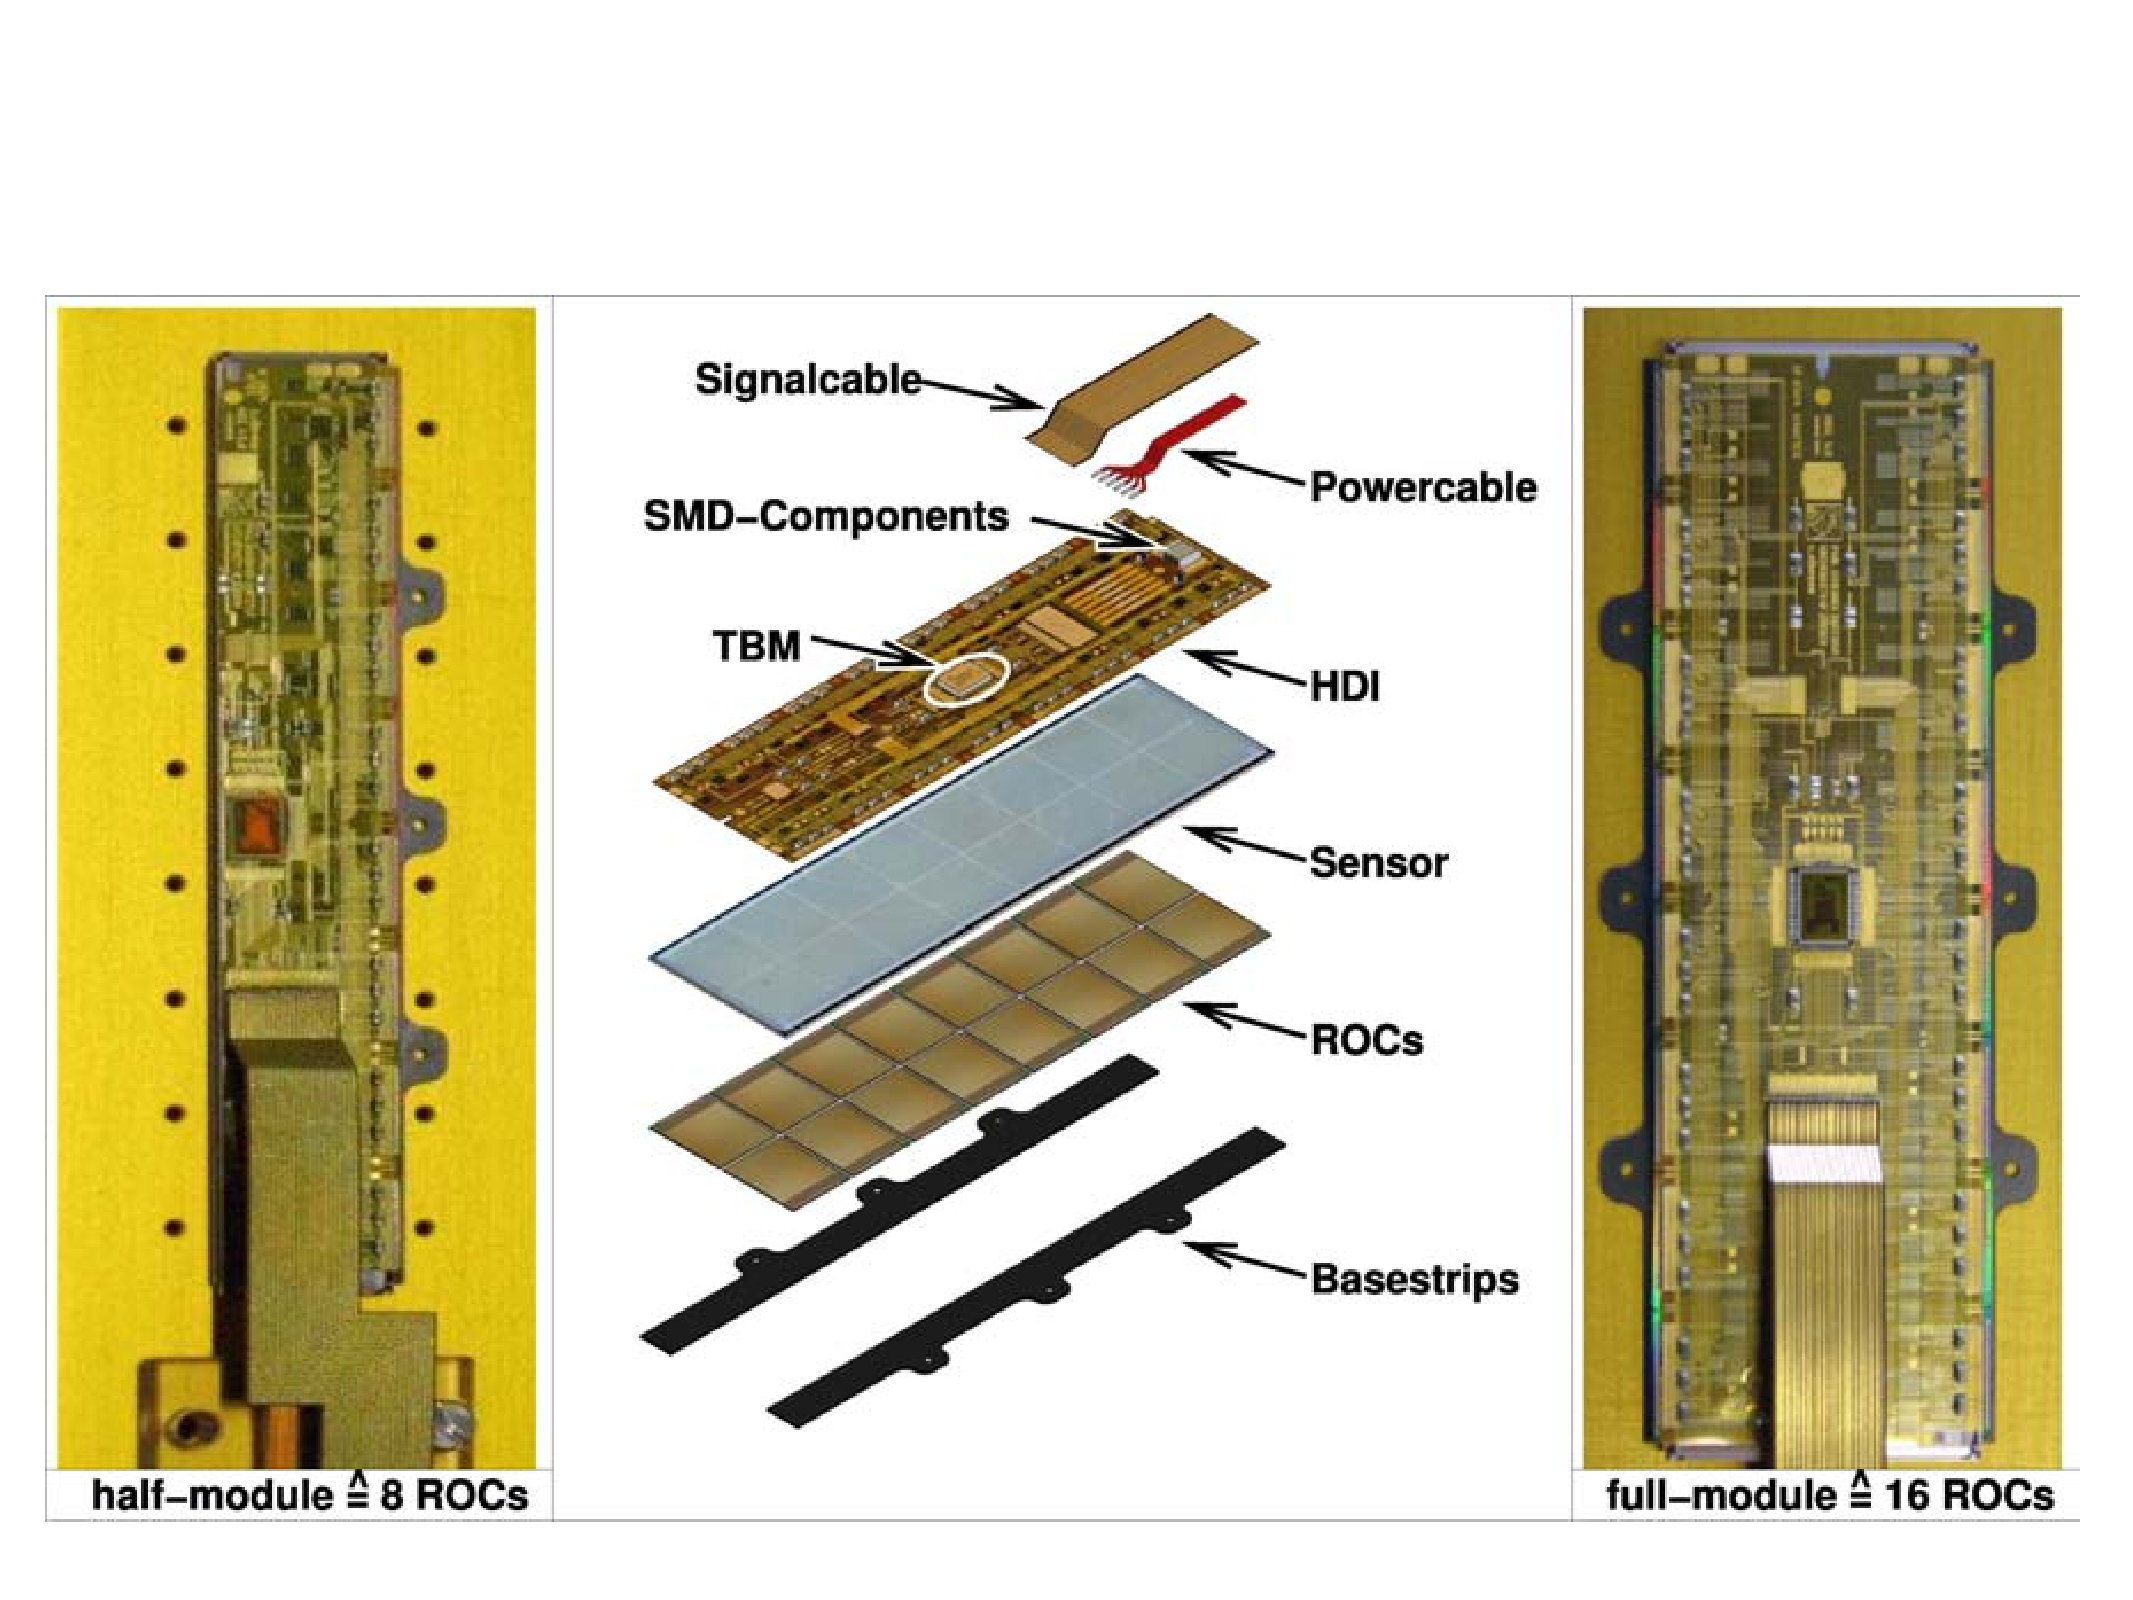
\includegraphics[width=0.99\textwidth]{CMS_DetectorFigures/BPixModule.pdf}
 \caption{BPix completed modules; (left) half-module, (center) an
   schematic of the different component forming the a full-module,(right) full-module.\label{fig:Bpix}}
\end{figure}
\begin{figure}
 \centering
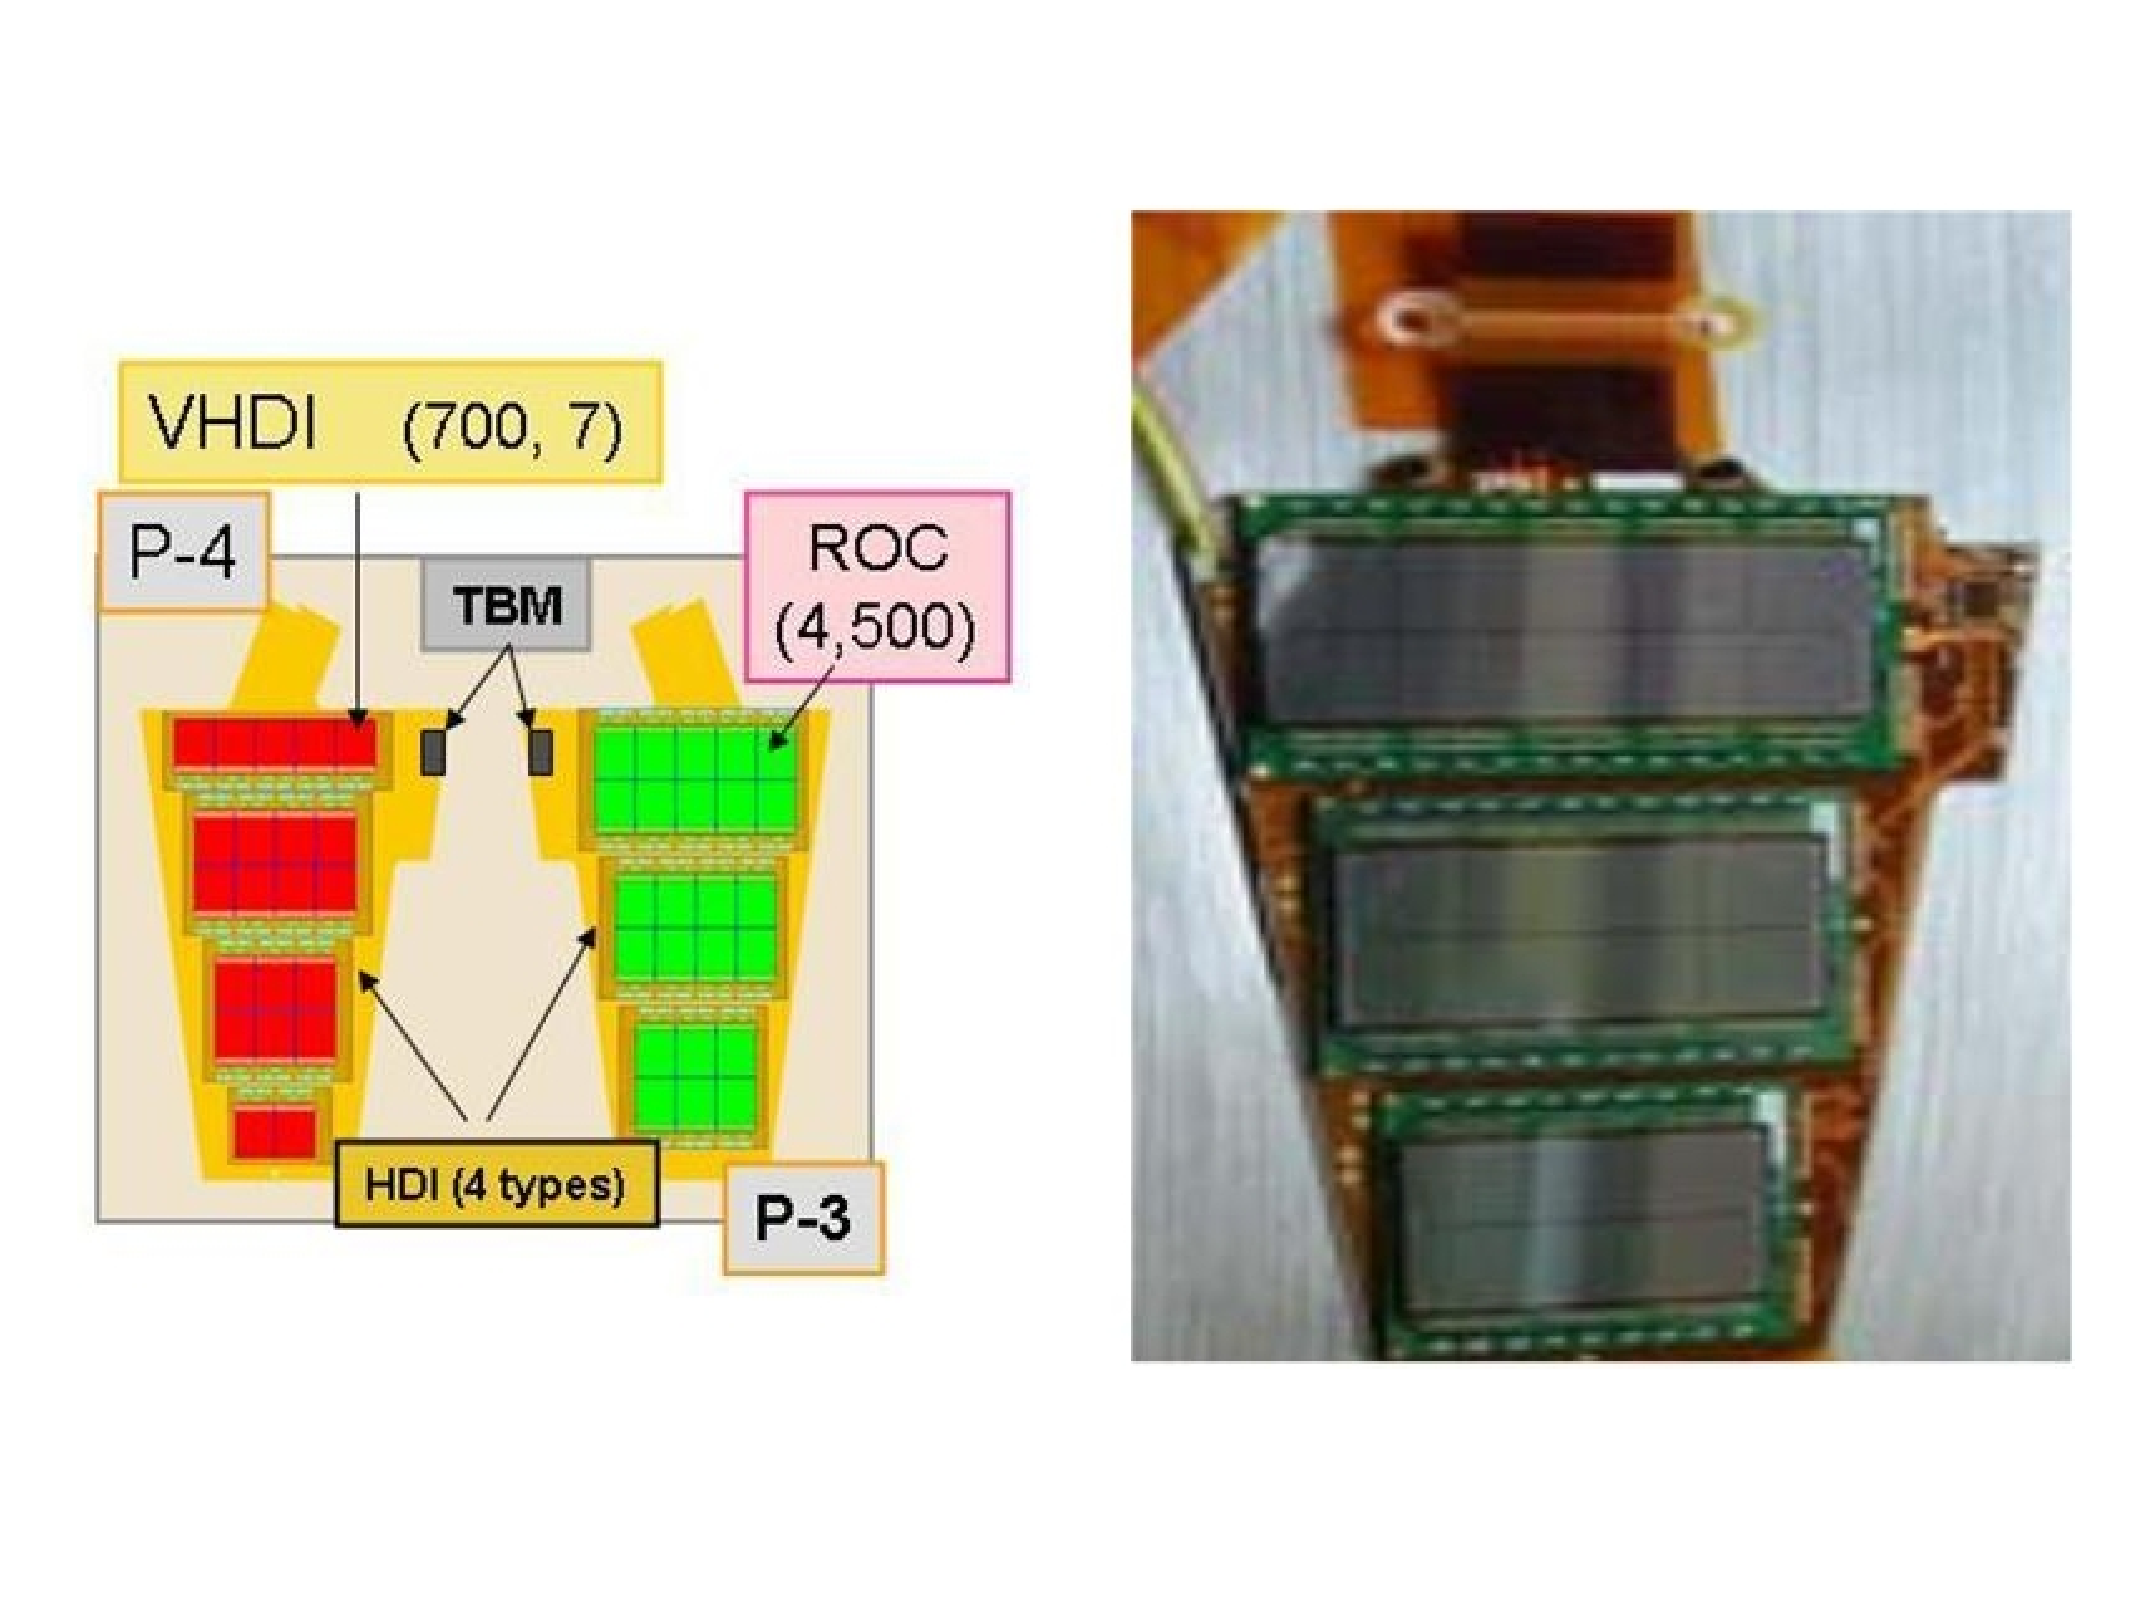
\includegraphics[width=0.99\textwidth]{CMS_DetectorFigures/FPixModule.pdf}
 \caption{FPix module; (left) an schematic of the two types of module,
   (right) a photograph of one of the completed FPix modules.\label{fig:Fpix}}
\end{figure}

\begin{figure}
 \centering
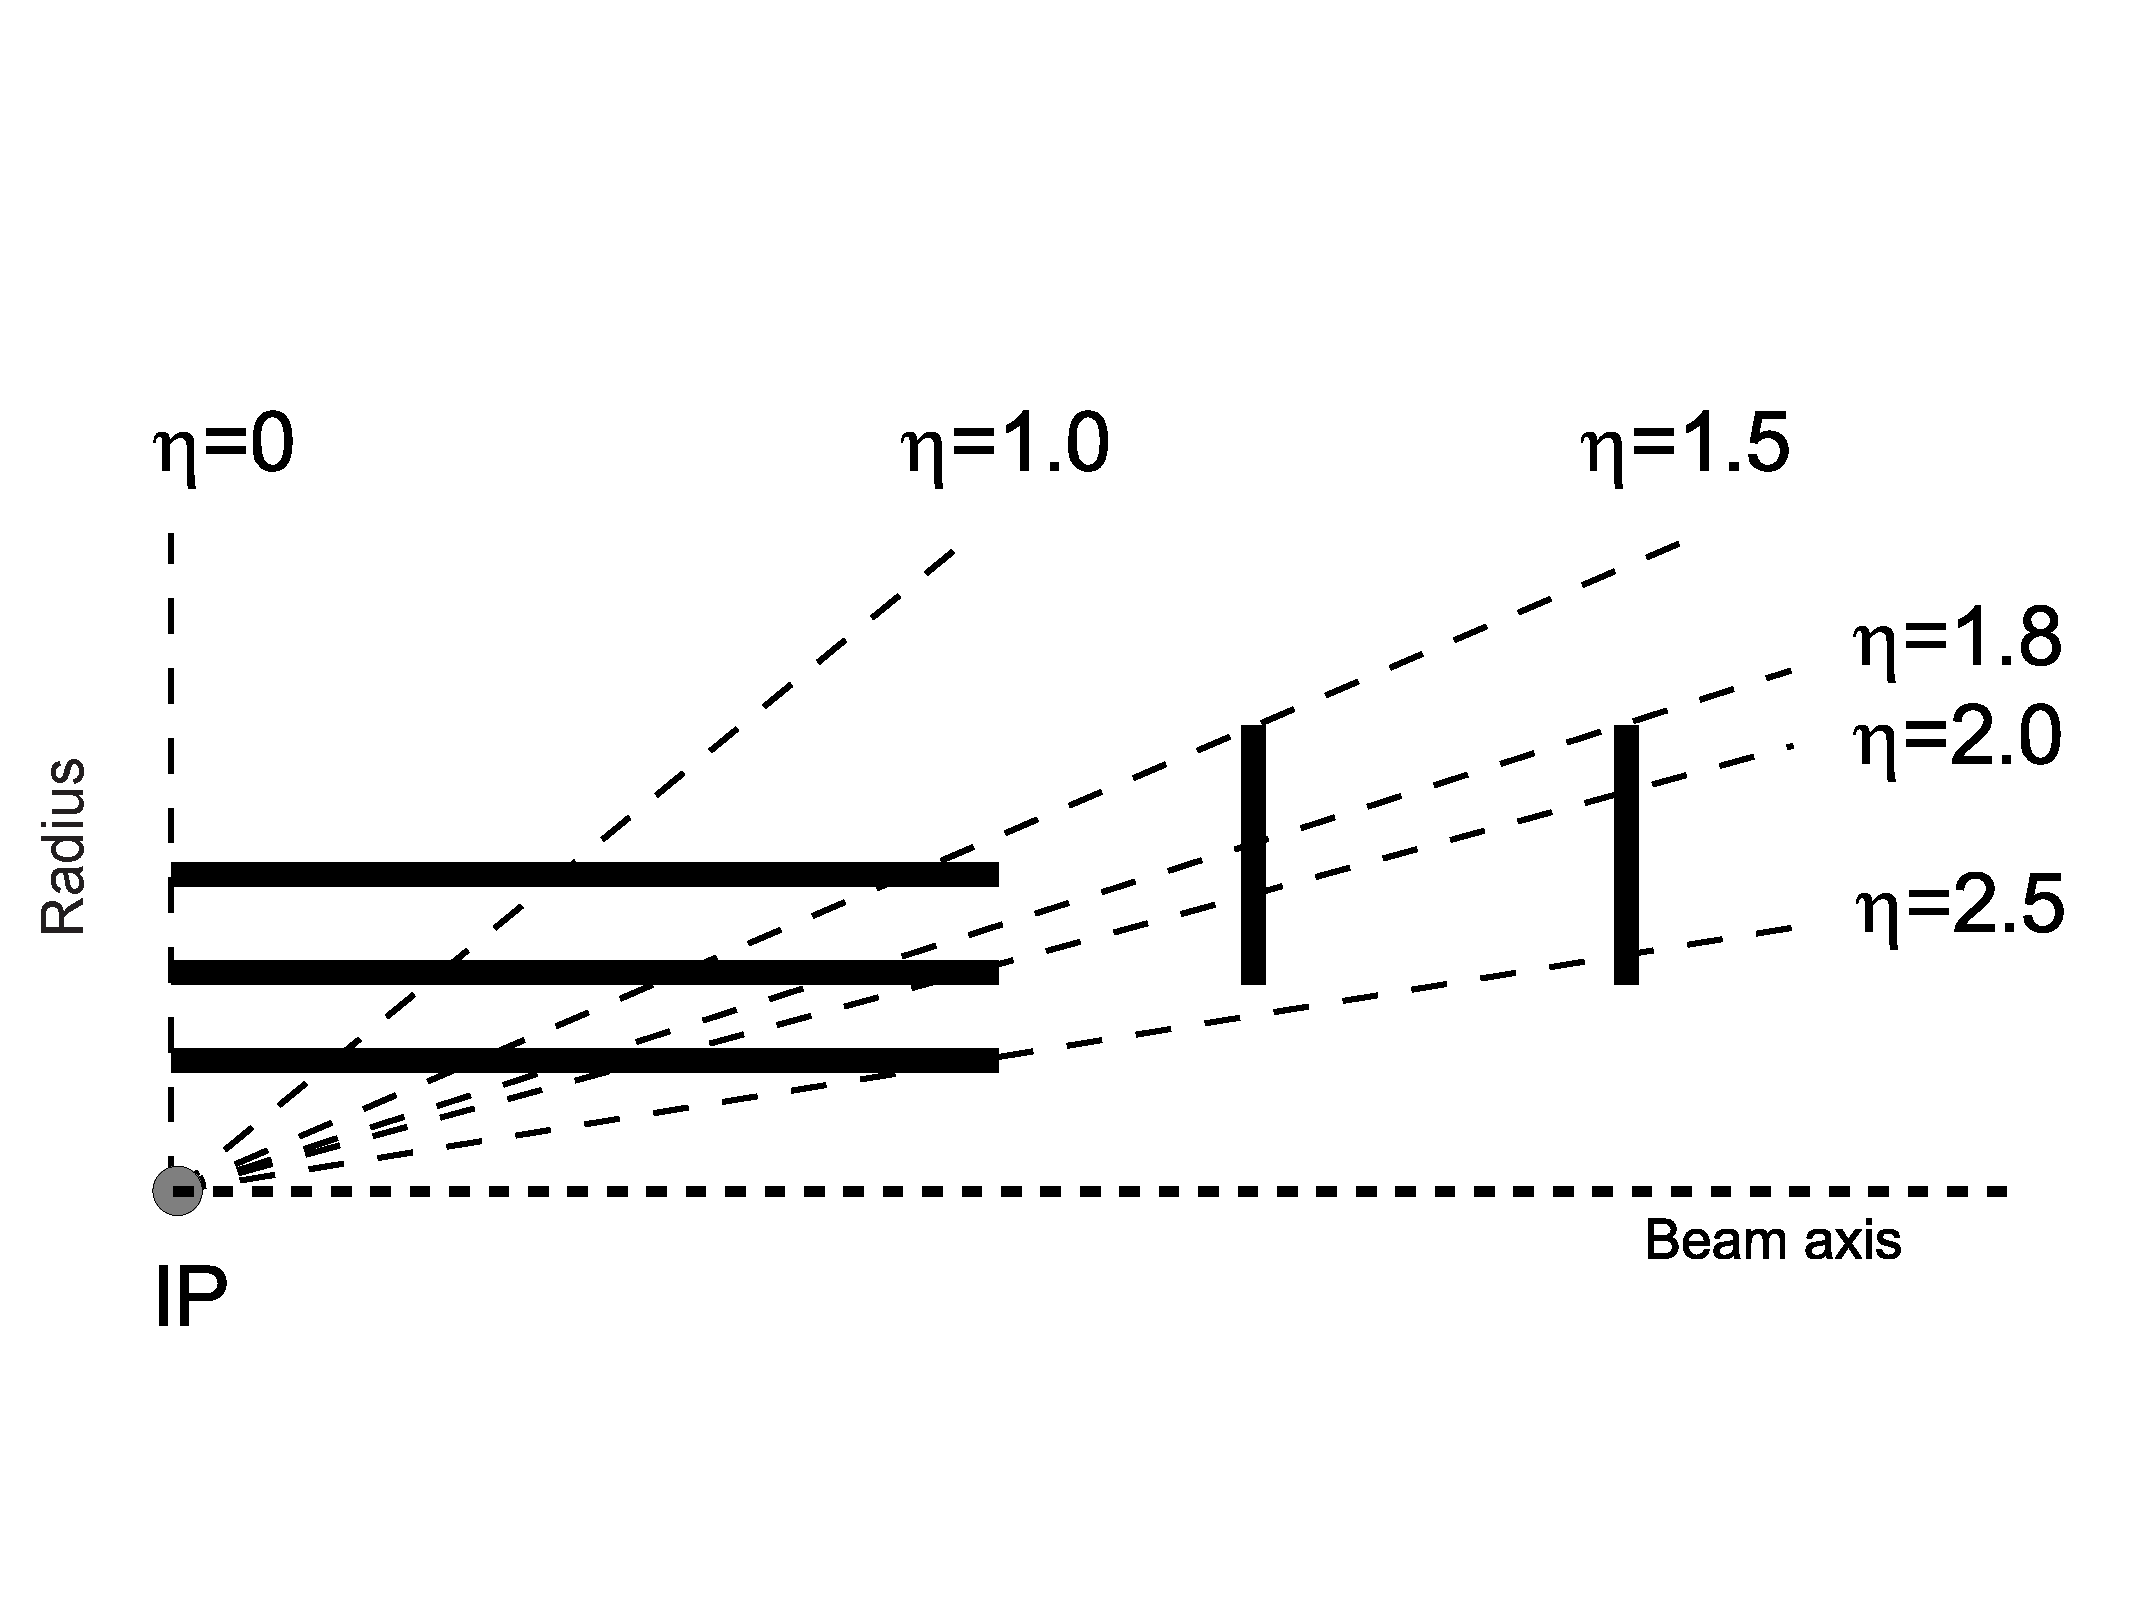
\includegraphics[width=0.49\textwidth]{CMS_DetectorFigures/PixelLayout.pdf}
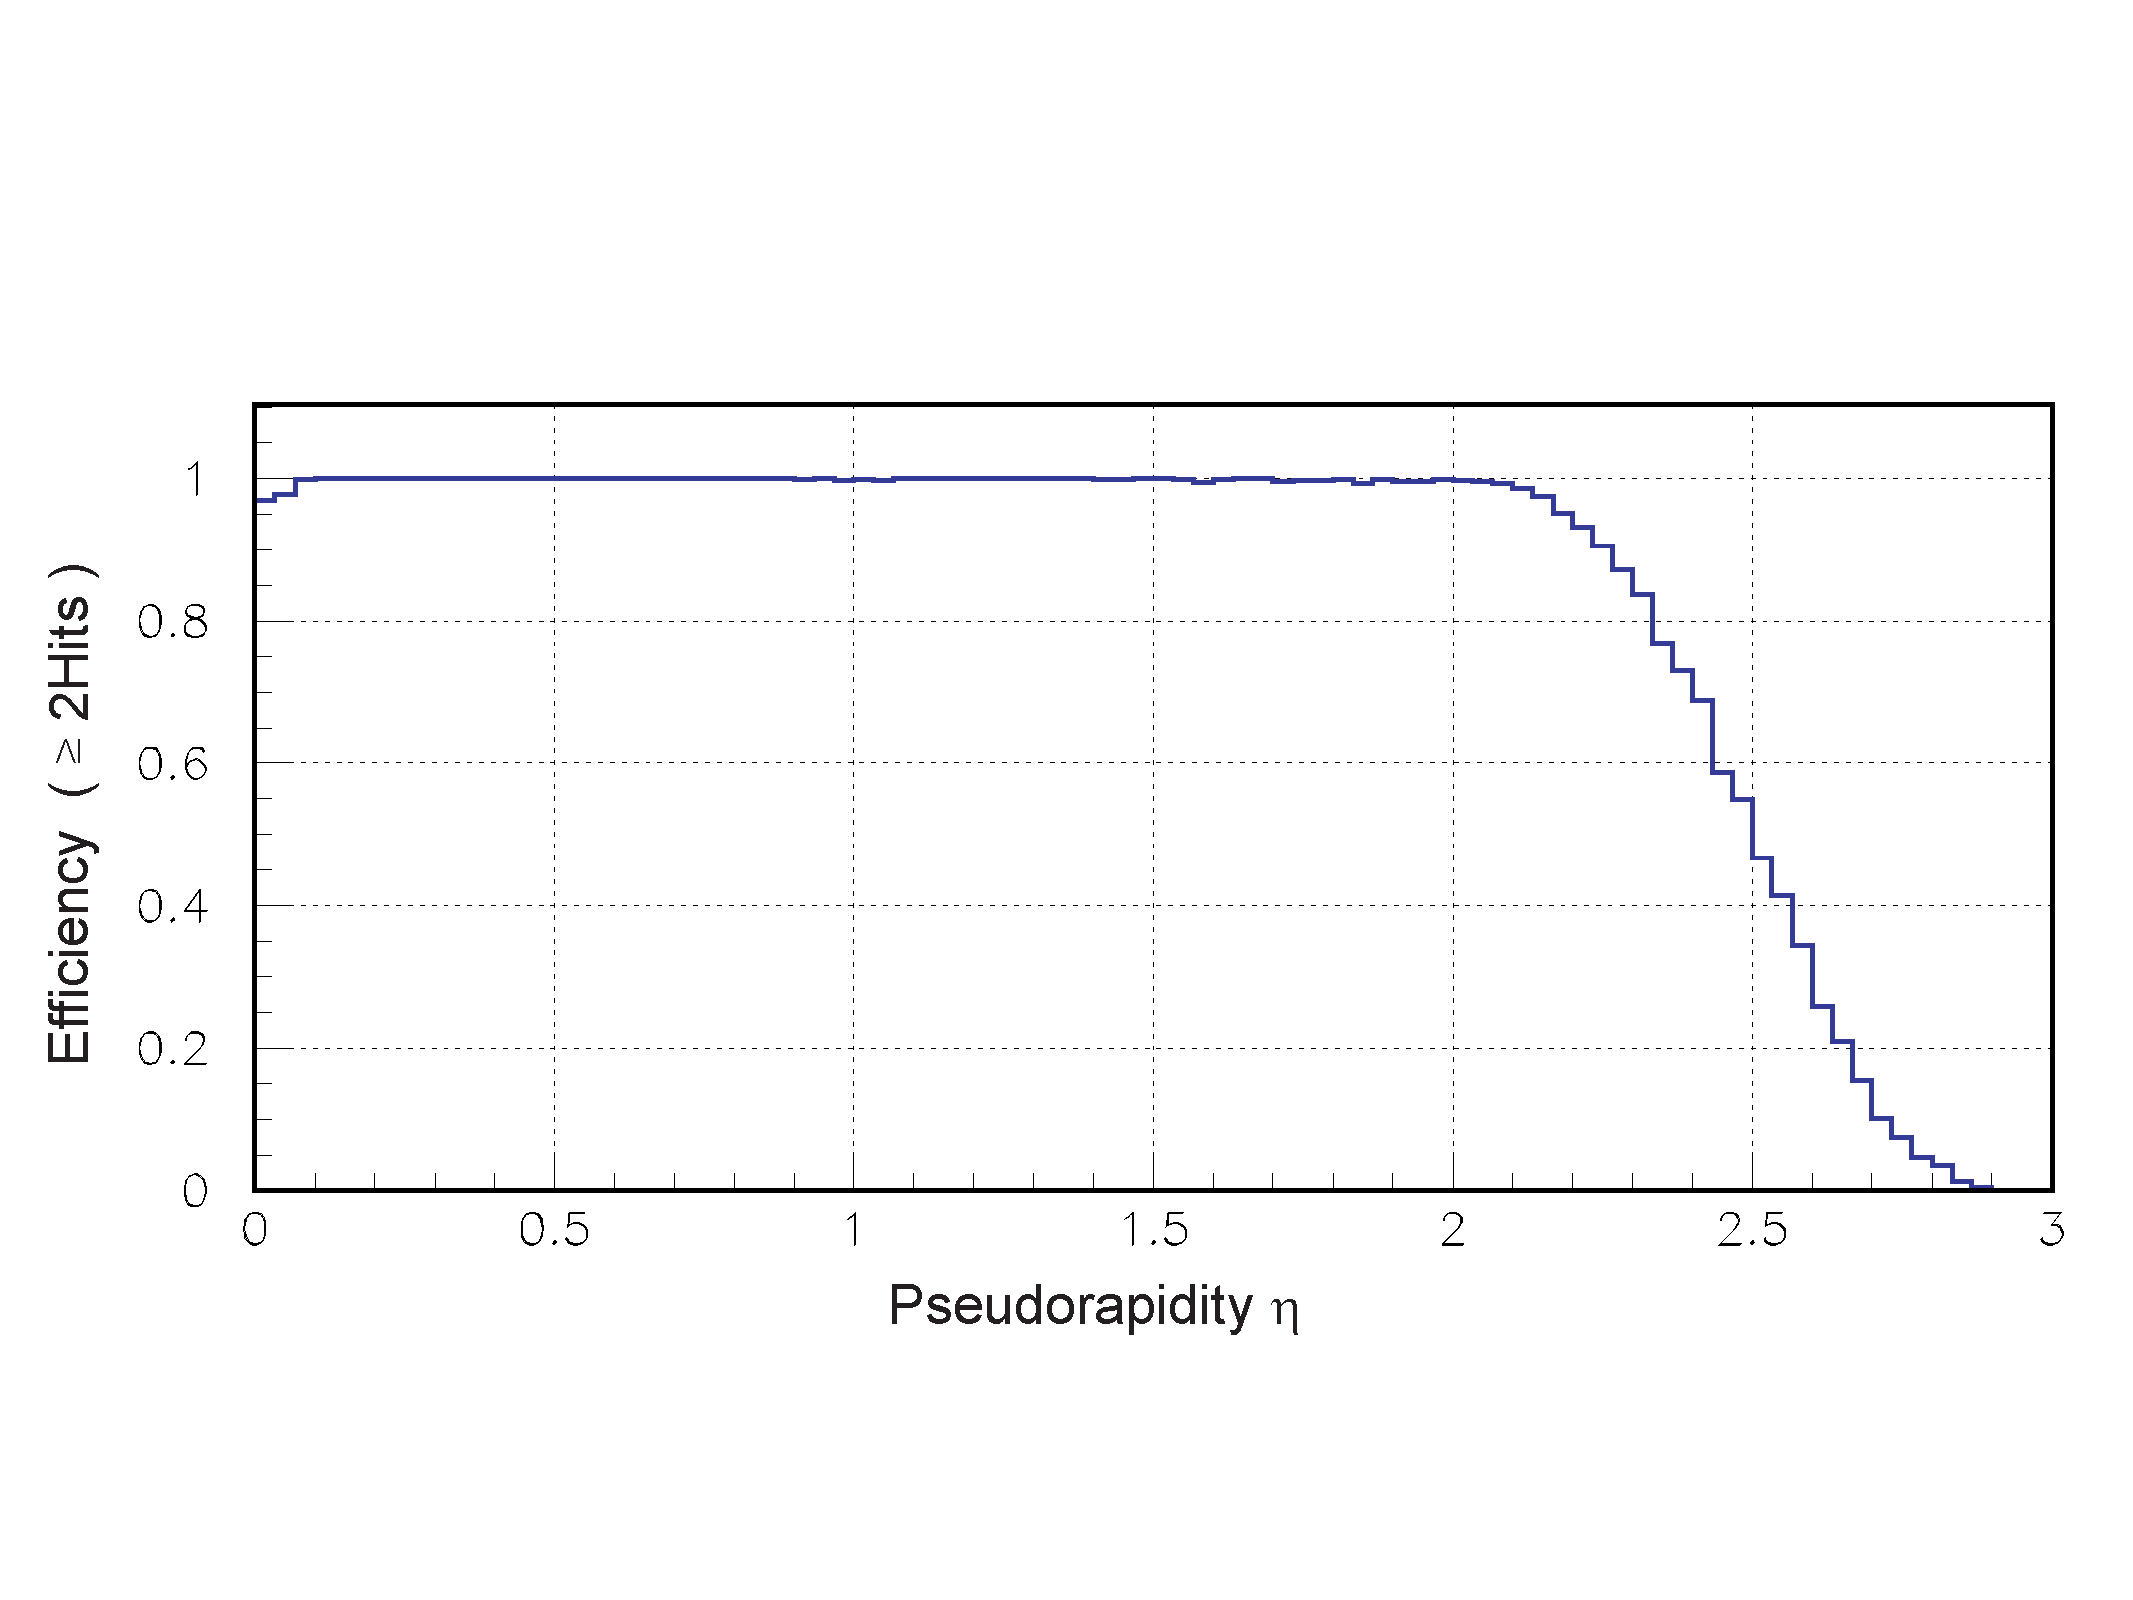
\includegraphics[width=0.49\textwidth]{CMS_DetectorFigures/PixelEfficiency.pdf}
 \caption{(Left) the layput of the silicon pixel tracker, (right) the
   pixel tracker detection efficiency as a function of the pseudorapidity.\label{fig:PixelLayout}}
\end{figure}
\subsection{Strip Tracker}
The silicon tracker is located outside the inner pixel tracker and is
composed of three subsystems that extend from 20 cm to 116 cm in the
radial direction. The Tracker Inner Barrel and Disks (TIB/TID) are
the innermost subsystem extending up to a radius of 55 cm, it includes
4 barrel layers and 3 disks at each side. The TIB/TID with their 320
$\mu$m thick silicon micro-strip sensor oriented along the $z$-axis records up to 4 $r$-$\phi$
measurements on a particle's trajectory. The strips pitch  in the TIB -- the
distance between each strip -- varies between 80 $\mu$m and 120 $\mu$m
in layers 1-2 and 3-4, respectively. The resulting single point
resolution is therefore 23 $\mu$m and 35 $\mu$m for the 1-2 and 3-4
layers, respectively. The TID has strip pitches between 100 -140$\mu$m
-- resulting in single point resolution between 29-41 $\mu$m. The
TIB/TID is completely sorrounded by the Tracker Outer Barrel (TOB)
which with its 6 barrel layer extends up to a radious of 116 cm. The
layers are composed of 500 $\mu$m thick micro-strips sensor with
pitches of 183 $\mu$m and 122 $\mu$m for the firts 4  and last 2
layer, respectively -- recording up to 6 $r$-$\phi$
measurements on a particle's trajectory with single point resolutions of 53 $\mu$m
and $\mu$m, respectively. The TIB/TID and the TOB cover the region
with $|z|< 113$ cm, beyond this point (see
Figure~\ref{fig:trackerlayout}) the Tracker EndCaps (TEC$^{\pm}$) --
where the sign, obiously, represents the position on the $z$-axis --
extend from 124 cm $|z|< 282$ cm and 22.5 cm $|r|< 113.5$ cm. The TEC
consists of 9 disks which contains up to 7 rings of silicon
micro-strips, the later are 320 $\mu$m and 500 $\mu$m thick in the
inner 4 and outer 3 rings, respectively.
Additionally, modules in the two innermost layers in the TIB and TOB,
the two inner most rings of the TID, as well as rings 1,2 and 5 of the TECs are
equipped with a second micro-strip detector module that is mounted
back-to-back allowing measurements on the perpedicular coordinate --
i.e. $z$ and r in the barrel and the disks, respectively. In this
fashion at least $\approx$ 9 hits in the silicon strip tracker in the
$|\eta|<2.4$ range are ensure, with at least $\approx$ 4
two-dimensional measurements. The full strip tracker amounts to a
total of 9.3 million strips and covers an active are of silicon equal
to 198 m$^2$.

\subsection{Performance of the CMS Tracker}

The tracker efficiency for single muons is measured in 7\TeV data as a
function of the muon pseudorapidity $\eta$ and the number of
reconstructed vertices using the tag-and-probe technique on muons
decaying from Z bosons. The results are shown in
Figure~\ref{fig:MuonEfficiency}, where the muon efficiency is above
99\% within the tracker acceptance and up to 20 reconstructed
vertices. The muon transverse momentum and transverse impact
paramenter resolution as a function of  $\eta$ are estimated from the
CMS full simulation, the results are shown in left and right panel of
Figure~\ref{fig:MuonResolution}, respectively. The muon transverse
momentum resolution is about 1-3\% for $|\eta|<1.5$ for muons of
different energies. The transverse impact parameter is estimated to be
between $\sim$10-20 $\mu$m for a 100\GeV muon while the for 1\GeV muons the
resolution is between $\sim$ 80-250 $\mu$m.

\begin{figure}
 \centering
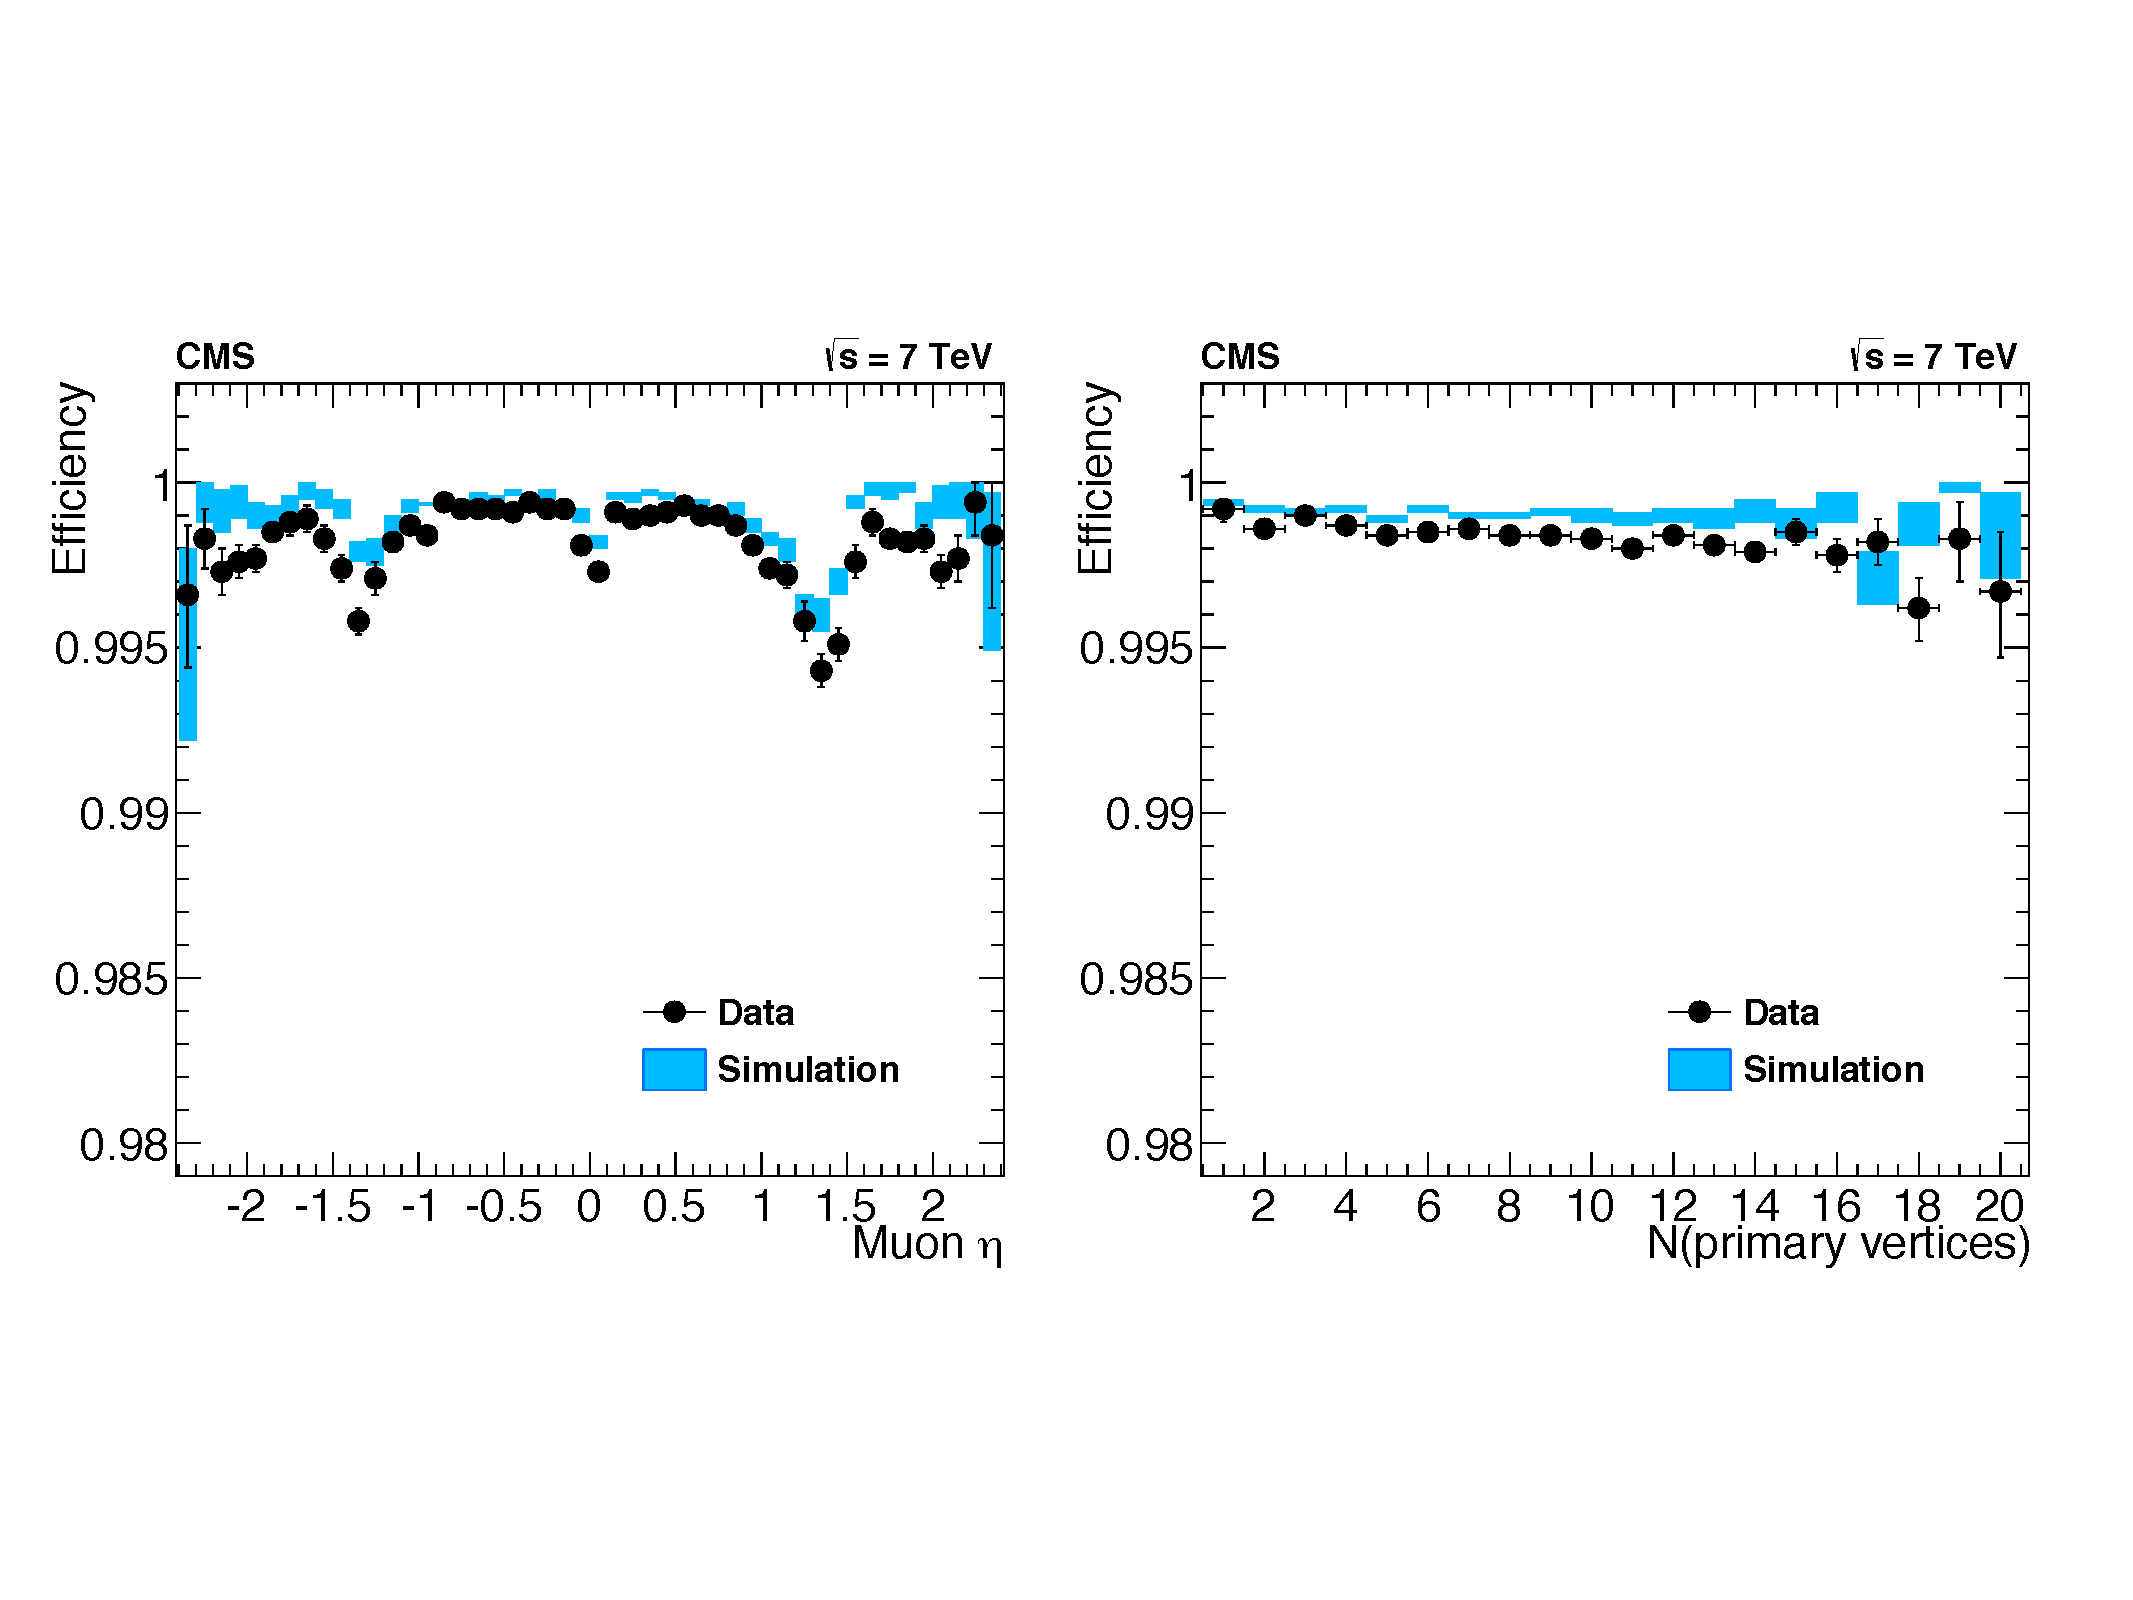
\includegraphics[width=0.99\textwidth]{CMS_DetectorFigures/TrackerMuonEff.pdf}
\caption{Tracking efficiency for muons from Z decays using the tag-and
 -probe technique. The left panel and right panel show the efficiency
 as function of the muon $\eta$ and the number of reconstructed
 vertices, respectively. The black dots represent the measurement in
 7\TeV data and the solid color represents the CMS simulation.\label{fig:MuonEfficiency}}
\end{figure}

\begin{figure}
 \centering
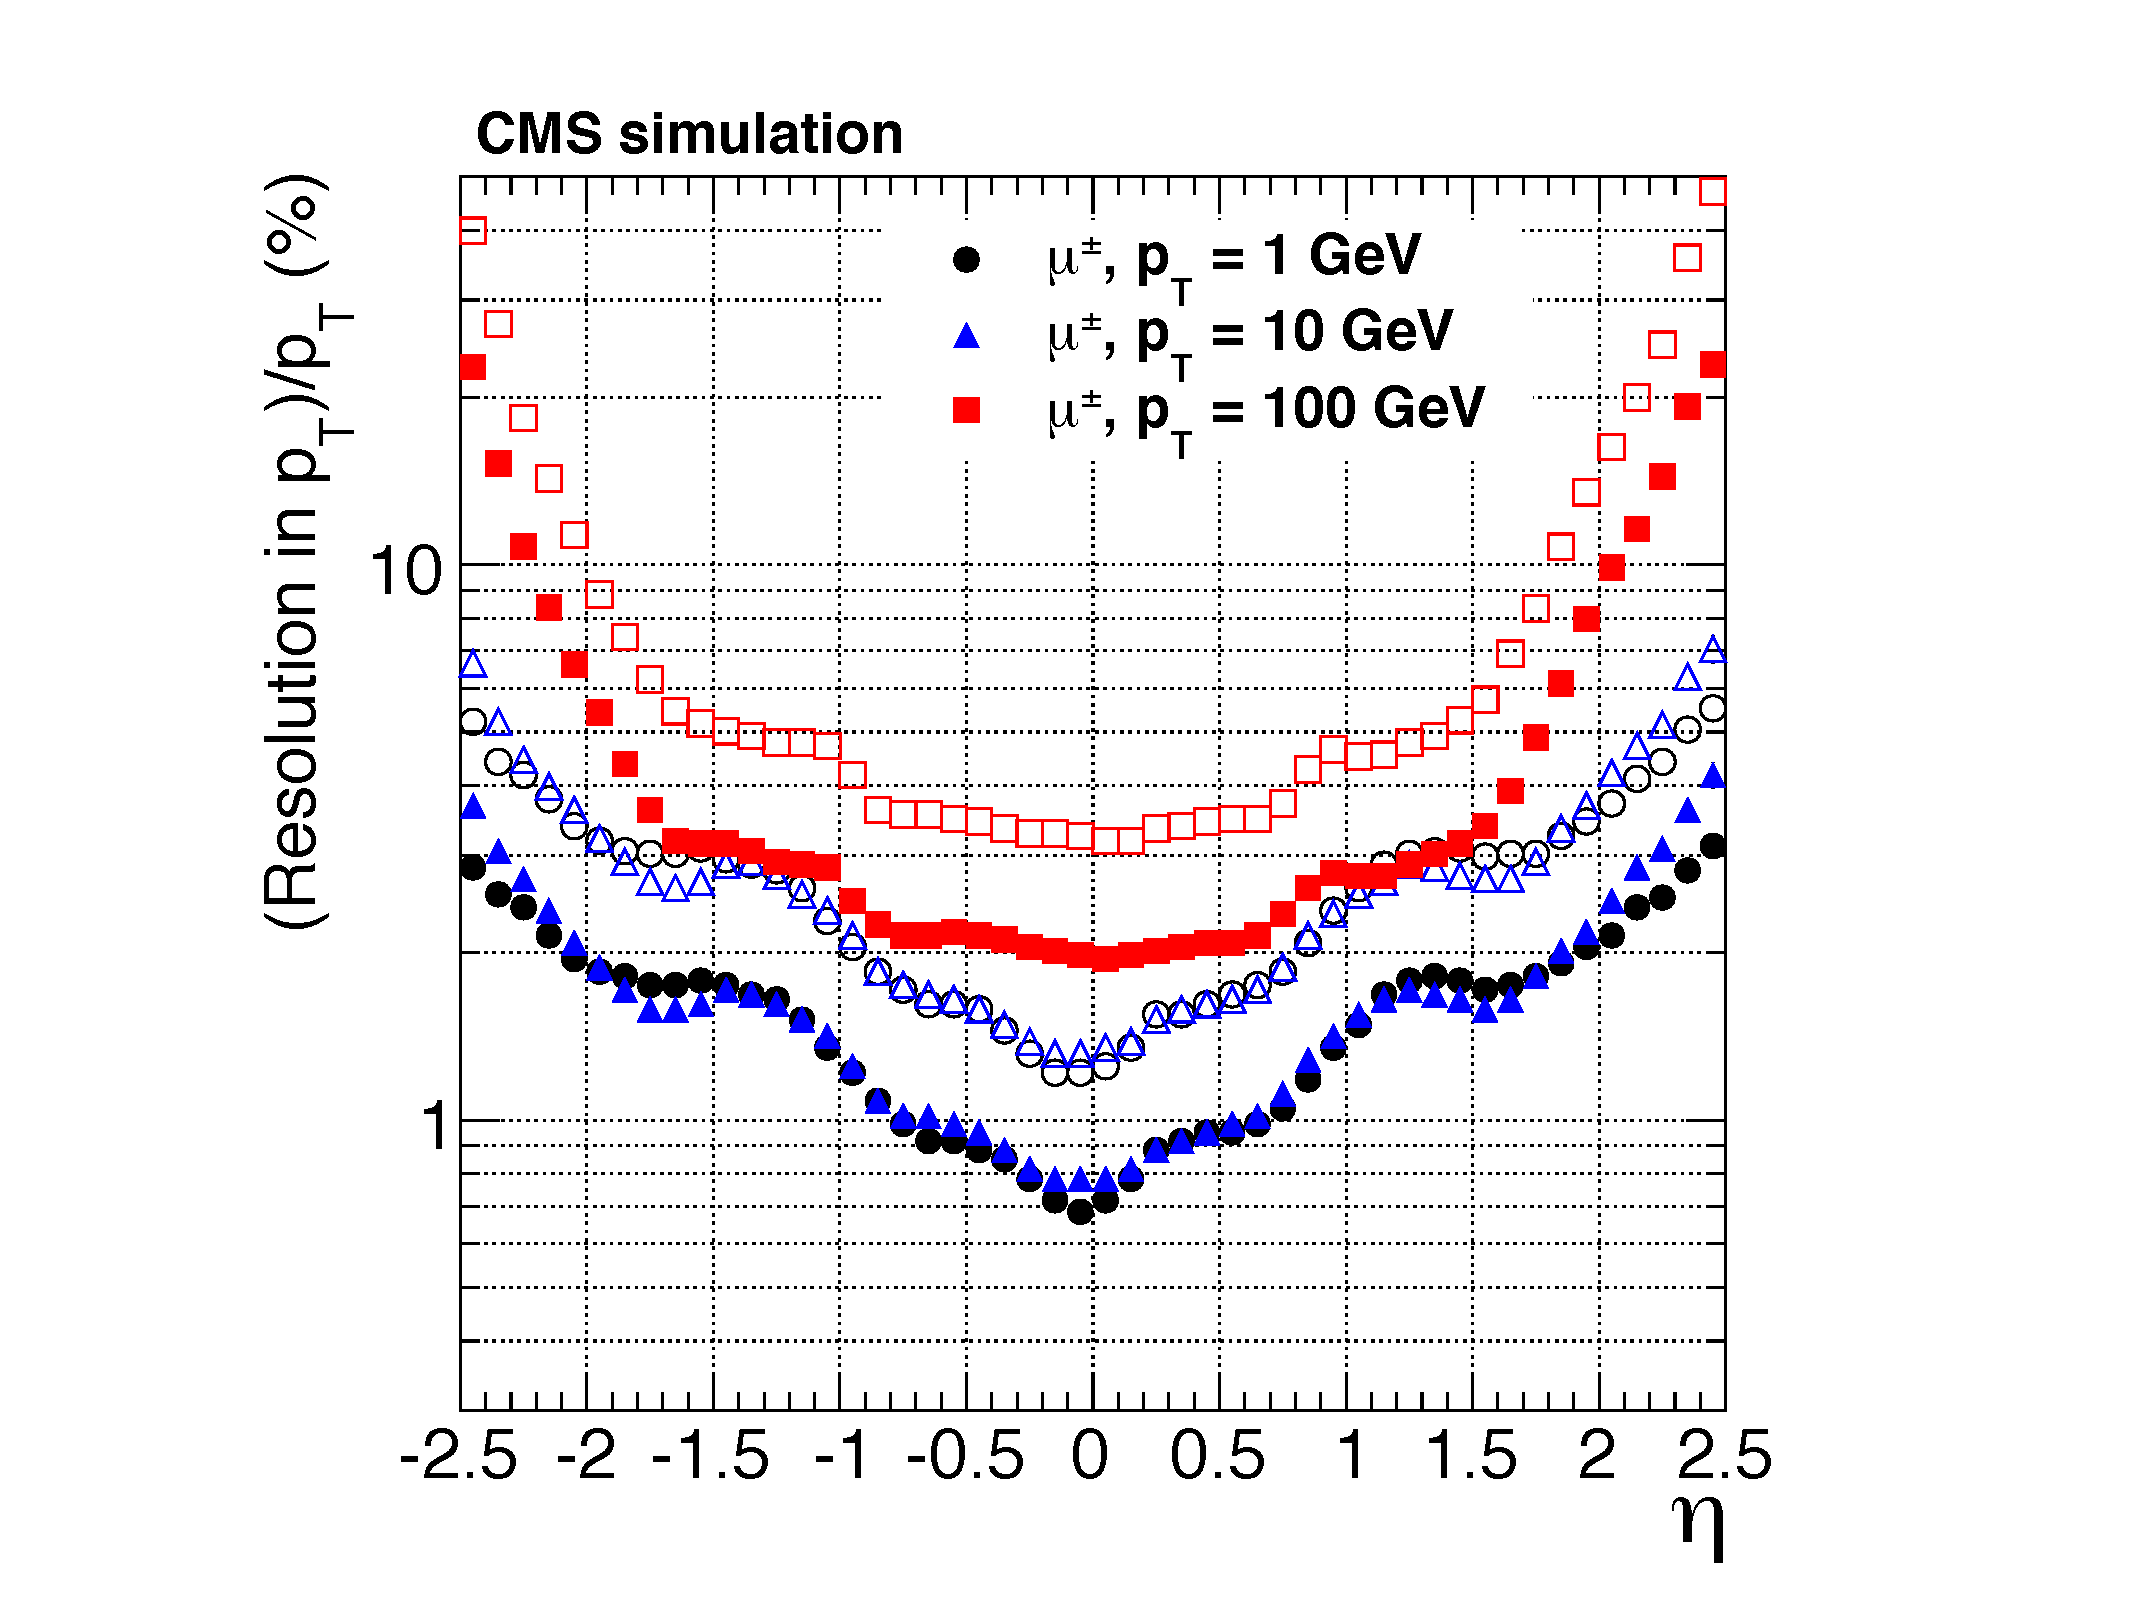
\includegraphics[width=0.49\textwidth]{CMS_DetectorFigures/TrackerPtResolution.pdf}
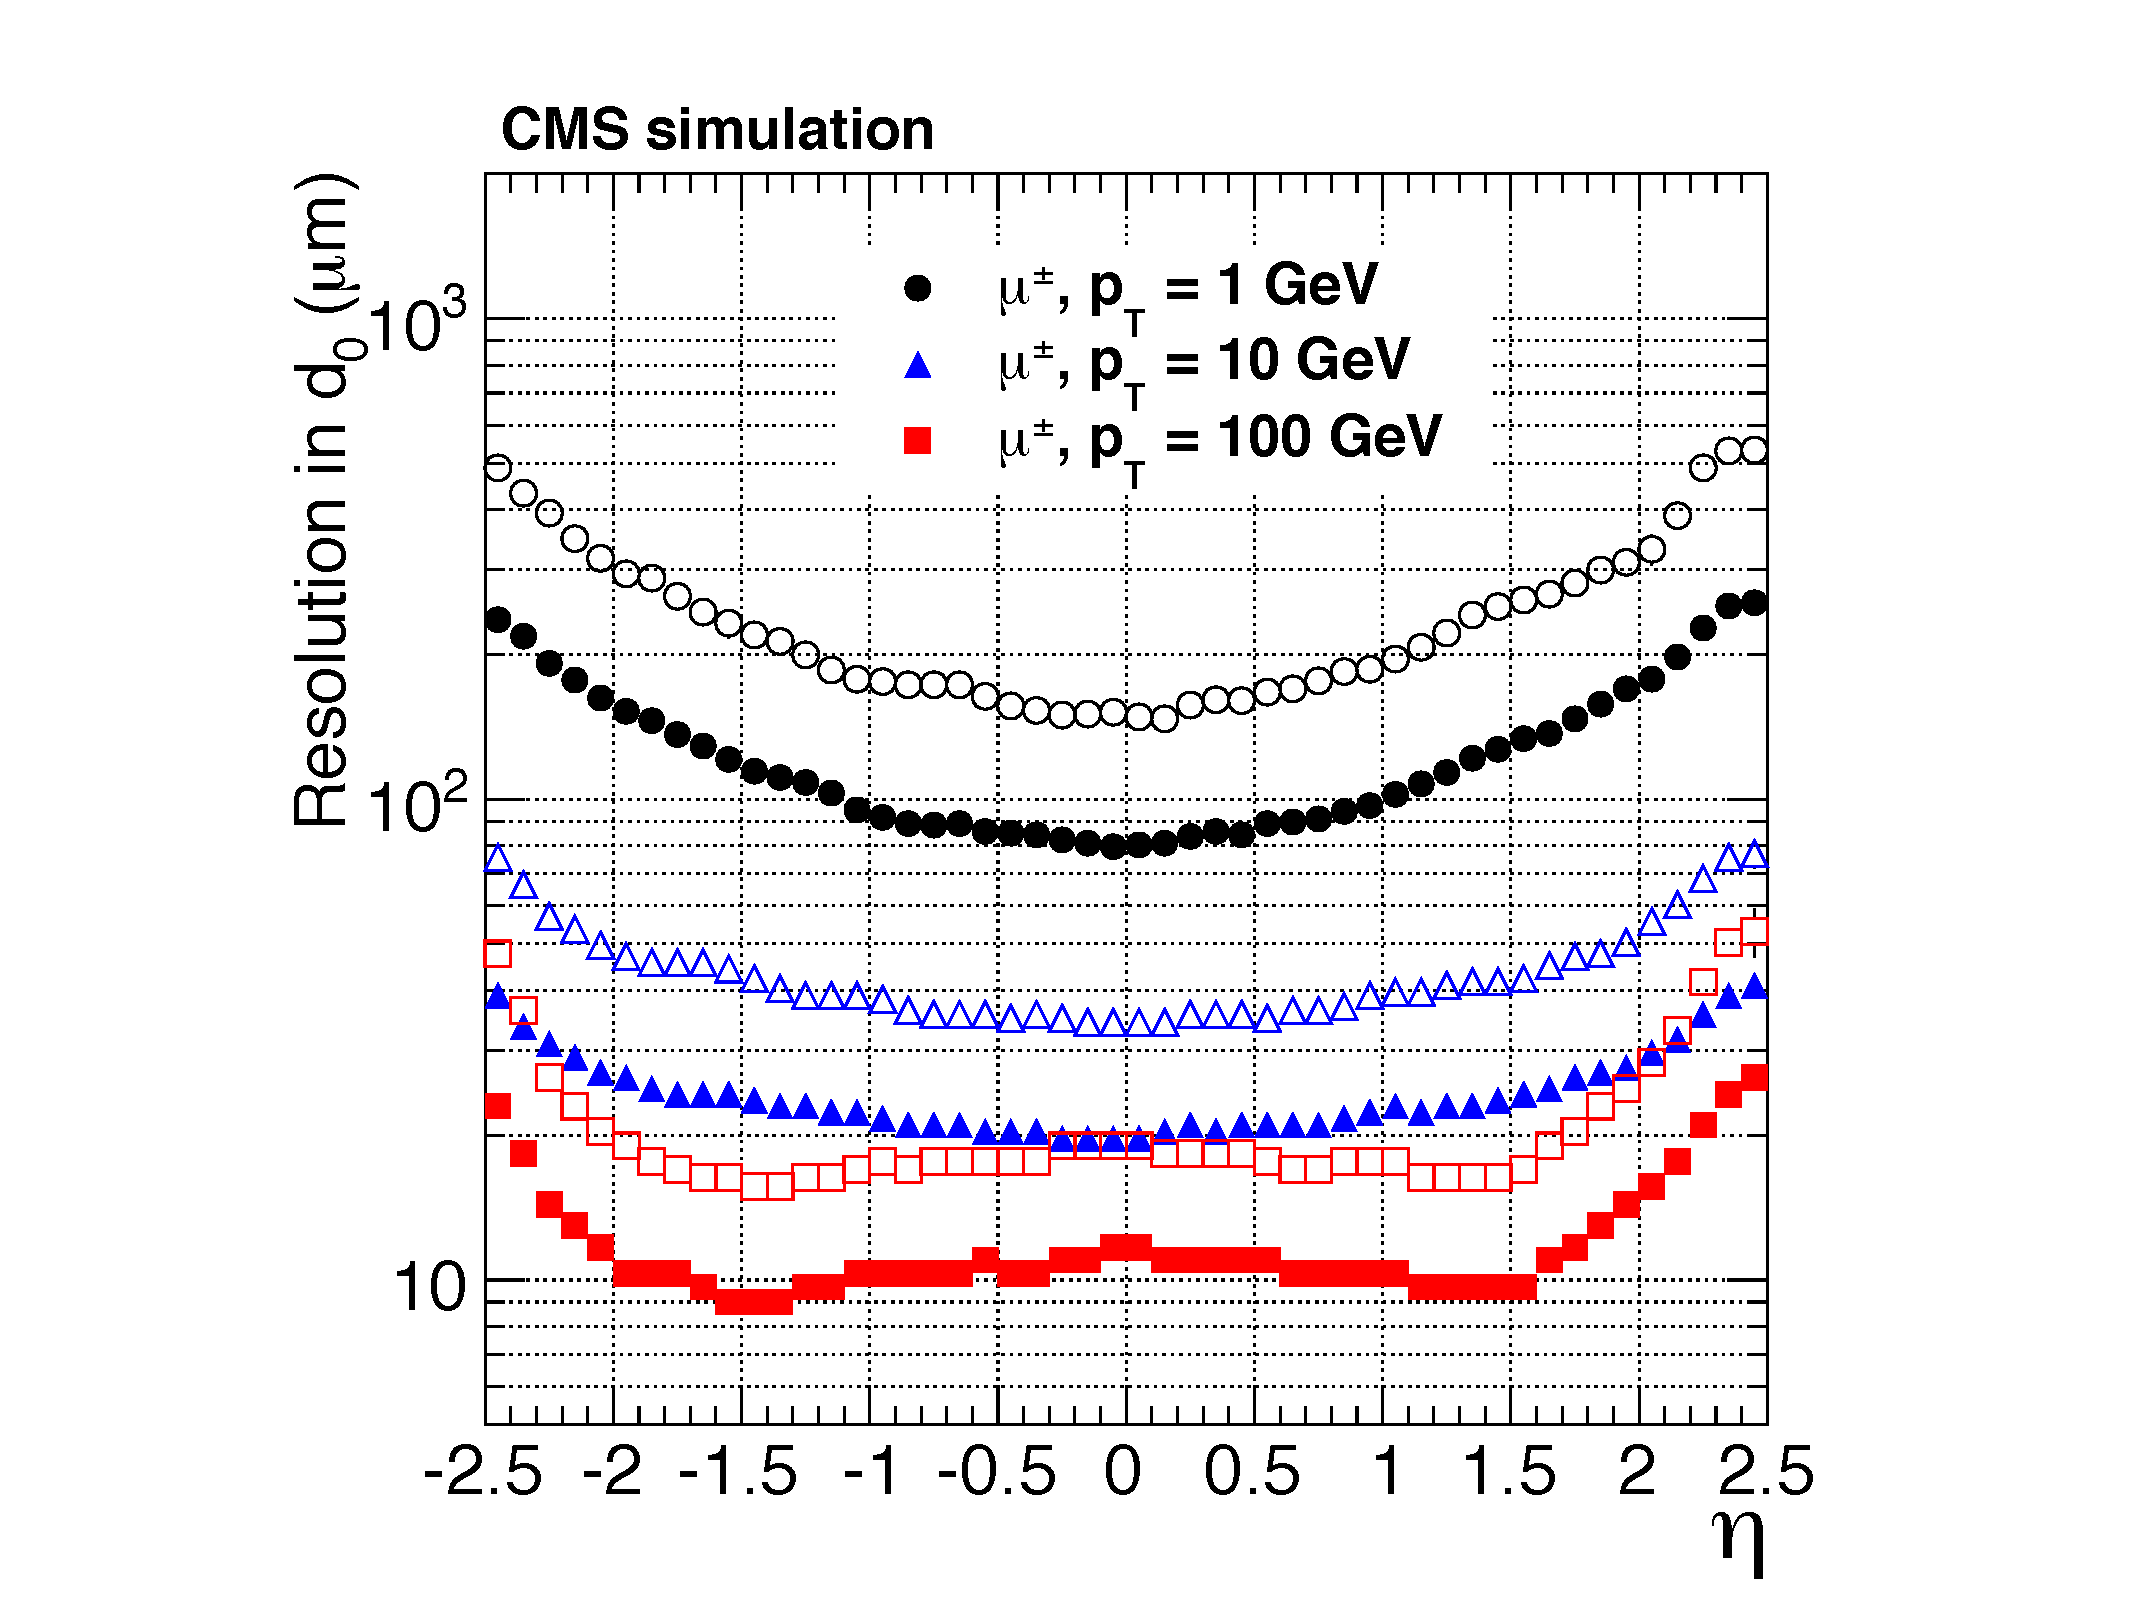
\includegraphics[width=0.49\textwidth]{CMS_DetectorFigures/TrackerImpactParameterResolution.pdf}
 \caption{Resolution as a function of the pseudorapidity $\eta$ for
   muons of $p_{\mathrm{T}} = $ 1, 10, and 100\GeV. The left panel
   shows the trasverse momentum resolution and the right panel the
   transverse impact parameter resolution. Both quantities are
   estimated from Simulation.\label{fig:MuonResolution}}
\end{figure}



\section{The Electromagnetic Calorimeter}
The CMS electromagnectic calorimeter (ECAL) is a granular and homogeneous
calorimeted built out of 61,200 lead tungstate (PbWO$_{4}$) crystals
in the barrel and closed by 7,324 PbWO$_{4}$ crystals in each of the
two endcaps. Additionally, a preshower detector is place in front of
the endcaps -- i.e. closer to the interaction point. The scintillating
light is collected by silicon avalanche photodiodes (APDs) in the ECAL barrel
(EB) and by vacuum phototriodes (VPTs) in the ECAL endcaps
(EE). Figure~\ref{fig:ECALgeometry} shows a projectional schematic
layout as well as a geometric view of a quarter of the CMS ECAL. The
ECAL excellent performance is one of the keystones of the physics
results of the CMS experiment, perhaps, best exemplyfied by the Higgs
boson search and characterization in the H$\rightarrow\gamma\gamma$
and H$\rightarrow$ZZ$^{*}$ decay channels~\cite{CMSHgg, CMSHzz}.

\begin{figure}
 \centering
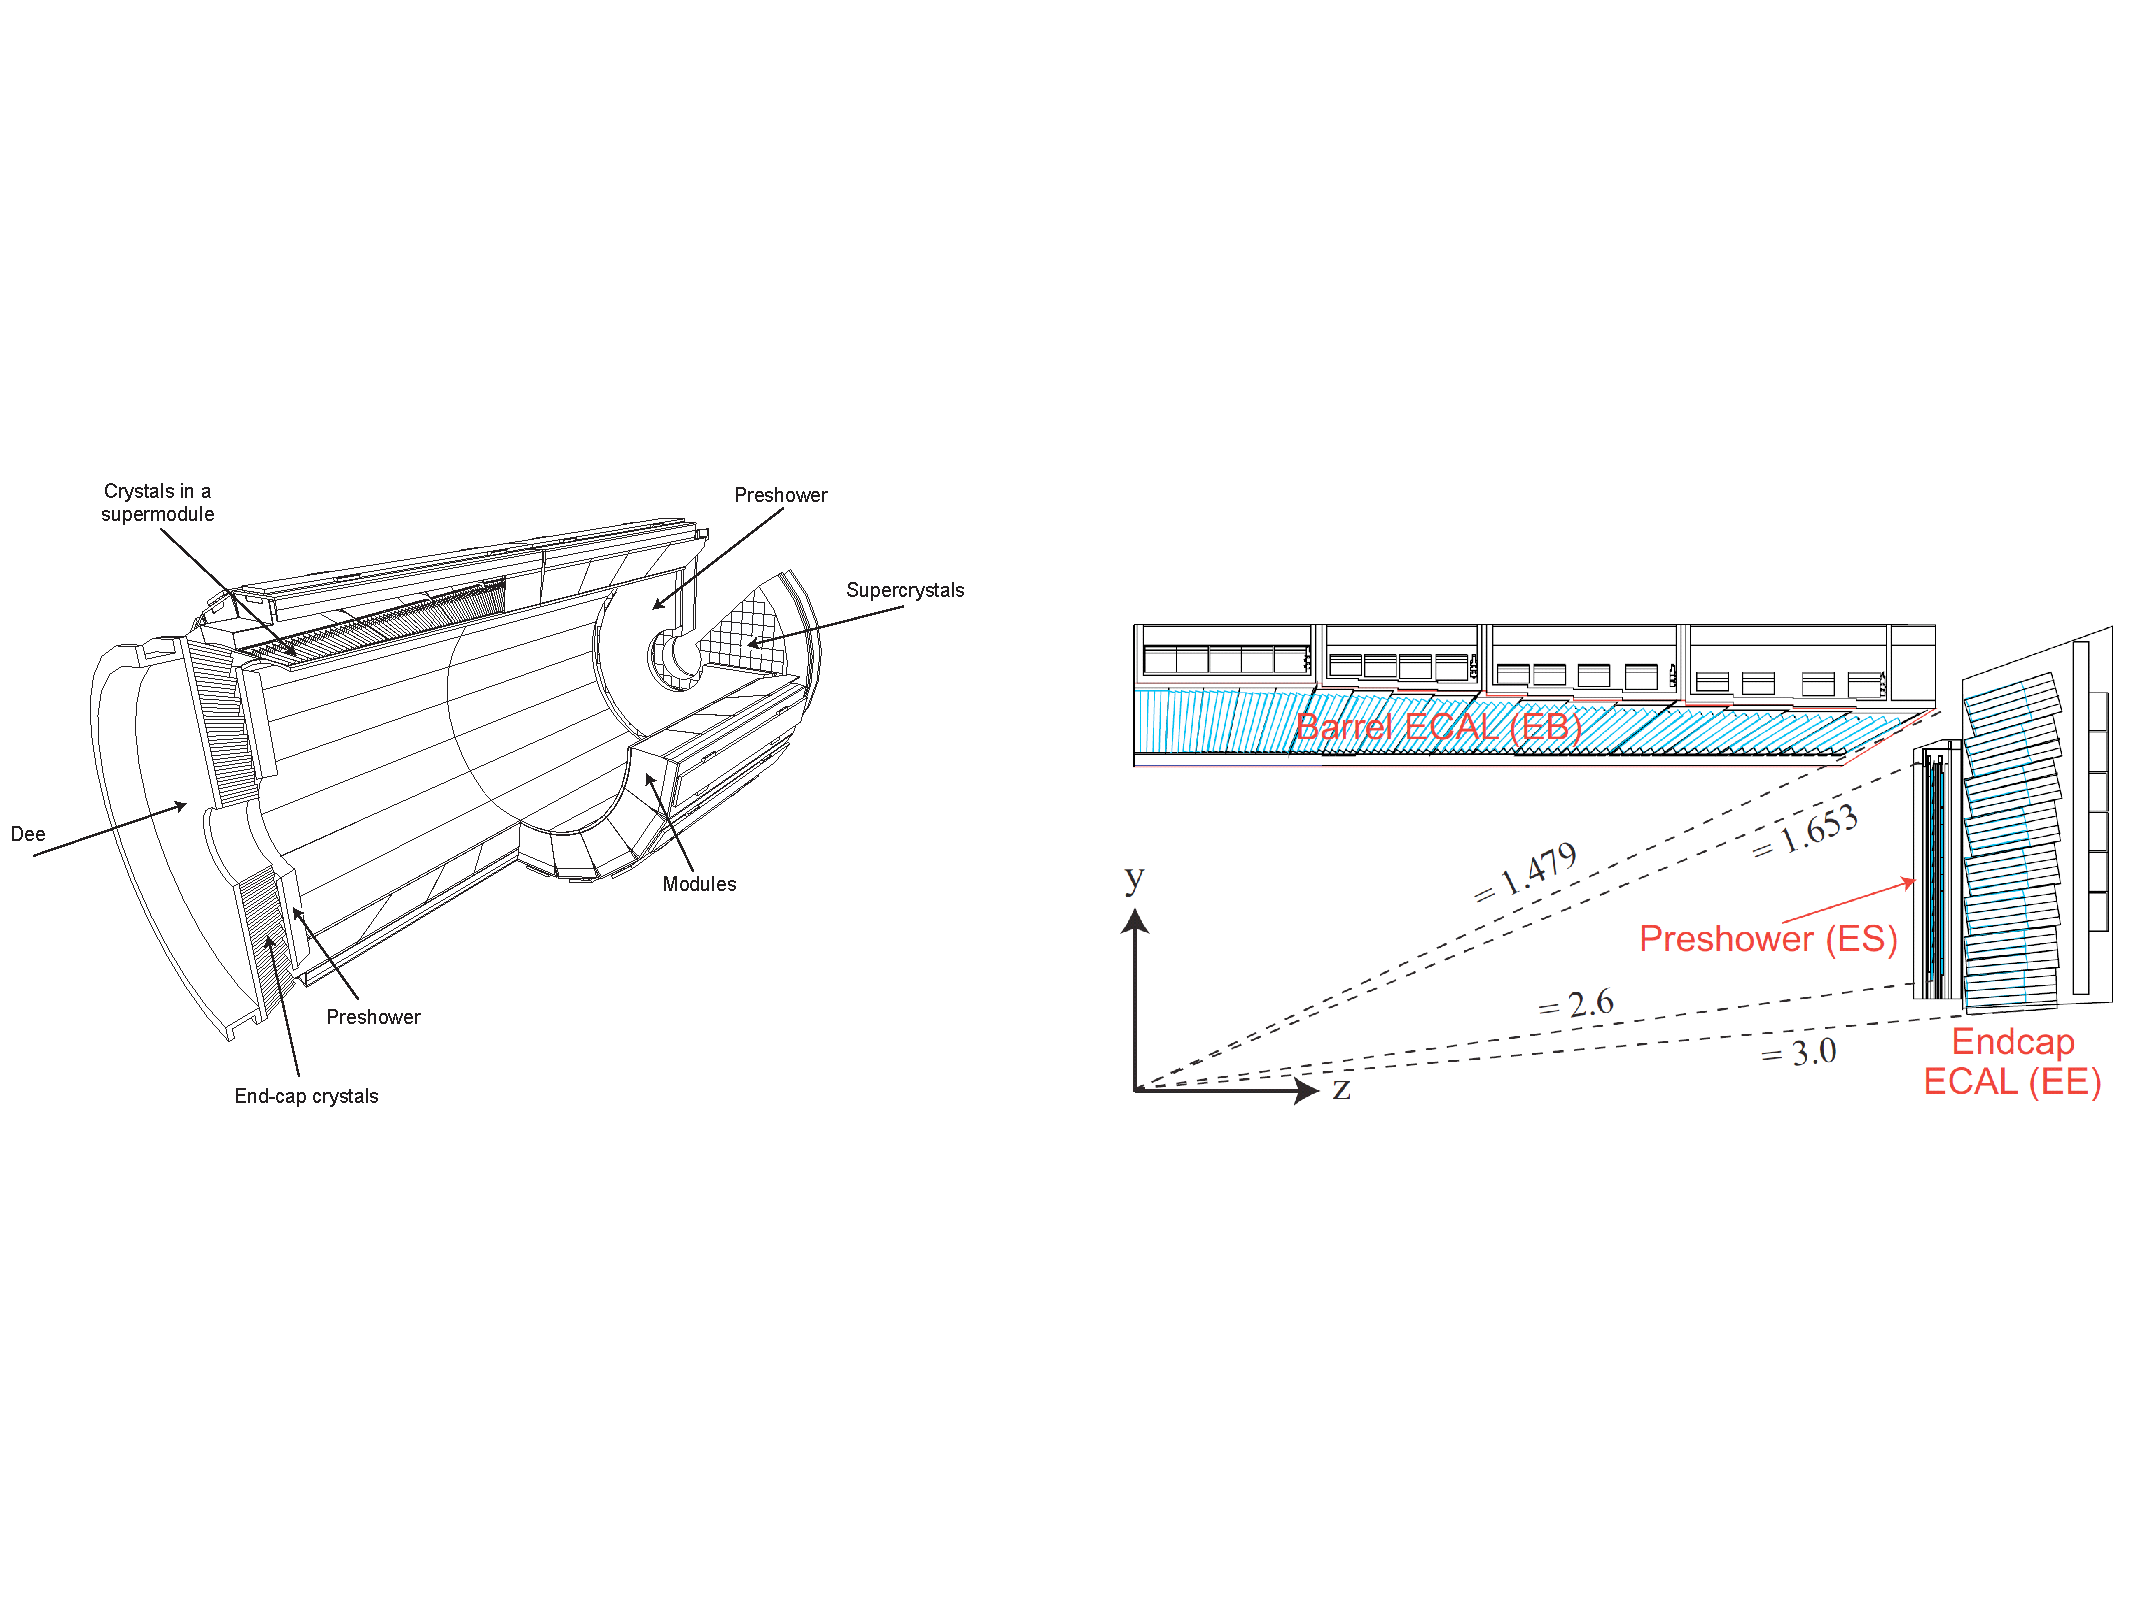
\includegraphics[width=0.99\textwidth]{CMS_DetectorFigures/ECAL_Geometry.pdf}
\caption{The layout of the CMS electromagnetic calorimenter. The left
  panel shows a projectional schematic
layout including all the major parts while the left panel shows a
geometric view of a quarter of the ECAL.\label{fig:ECALgeometry}}
\end{figure}

The PbWO$_{4}$ crystals with a density of 8.28 g/cm$^{3}$ provided a
good candidate because of its small radiation length ($X_{0} = 0.89$
cm), small moli\`ere radious (2.19 cm), and fast response. PbWO$_{4}$
crystals have a relatively low light yield of about 10
photo-electrons/MeV and therefore they required to be read out by
sensors with internal amplification inside the 3.8 T magnetic
field. The crystals in the EB are 23 cm long and have a
cross-sectional area of 2.2$\times$2.2 cm$^{2}$ (equivalent to
0.0174$\times$0.0174 in $\eta$, $\phi$), they are located at radious
of 1.29 m and arranged
in a quasi-projective geometry with 170 crystals -- 85 at each side --  covering up to a pseudorapidity range
$|\eta| < 1.48$. With 360 crytals in the $\phi$  direction the EB is
fully hermetic. The EE crystals are located at $z = \pm$ 315.4 cm, they
have a cross-sectional are of 2.86$\times$2.86 cm$^{2}$  and
3.0$\times$3.0 cm$^{2}$ at the front an rear faces, respectively, and
a length of 22 cm. They crystals are grouped in mechanical structure
of 5$\times$5 crystals and arranged in the traditional $x$-$y$
directions. Each endcap is divided into halves or \textit{Dees},
holding 3,662 crystals. The EE extends the ECAL coverage up to the
range $1.479 < |\eta| < 3.0$. The left and right panels of
Figure~\ref{fig:ECALcrystals} show the EB crystal instrumented with an
APD ant the EE crystal instrumented with a VPT, respectively.  Real
photographs of an EB module equipped with crystal is presented in
Figure~\ref{fig:ECALEB_module} while an EE Dee fully instrumented with crystals is shown
in Figure~\ref{fig:ECALEE_module}.
\begin{figure}
 \centering
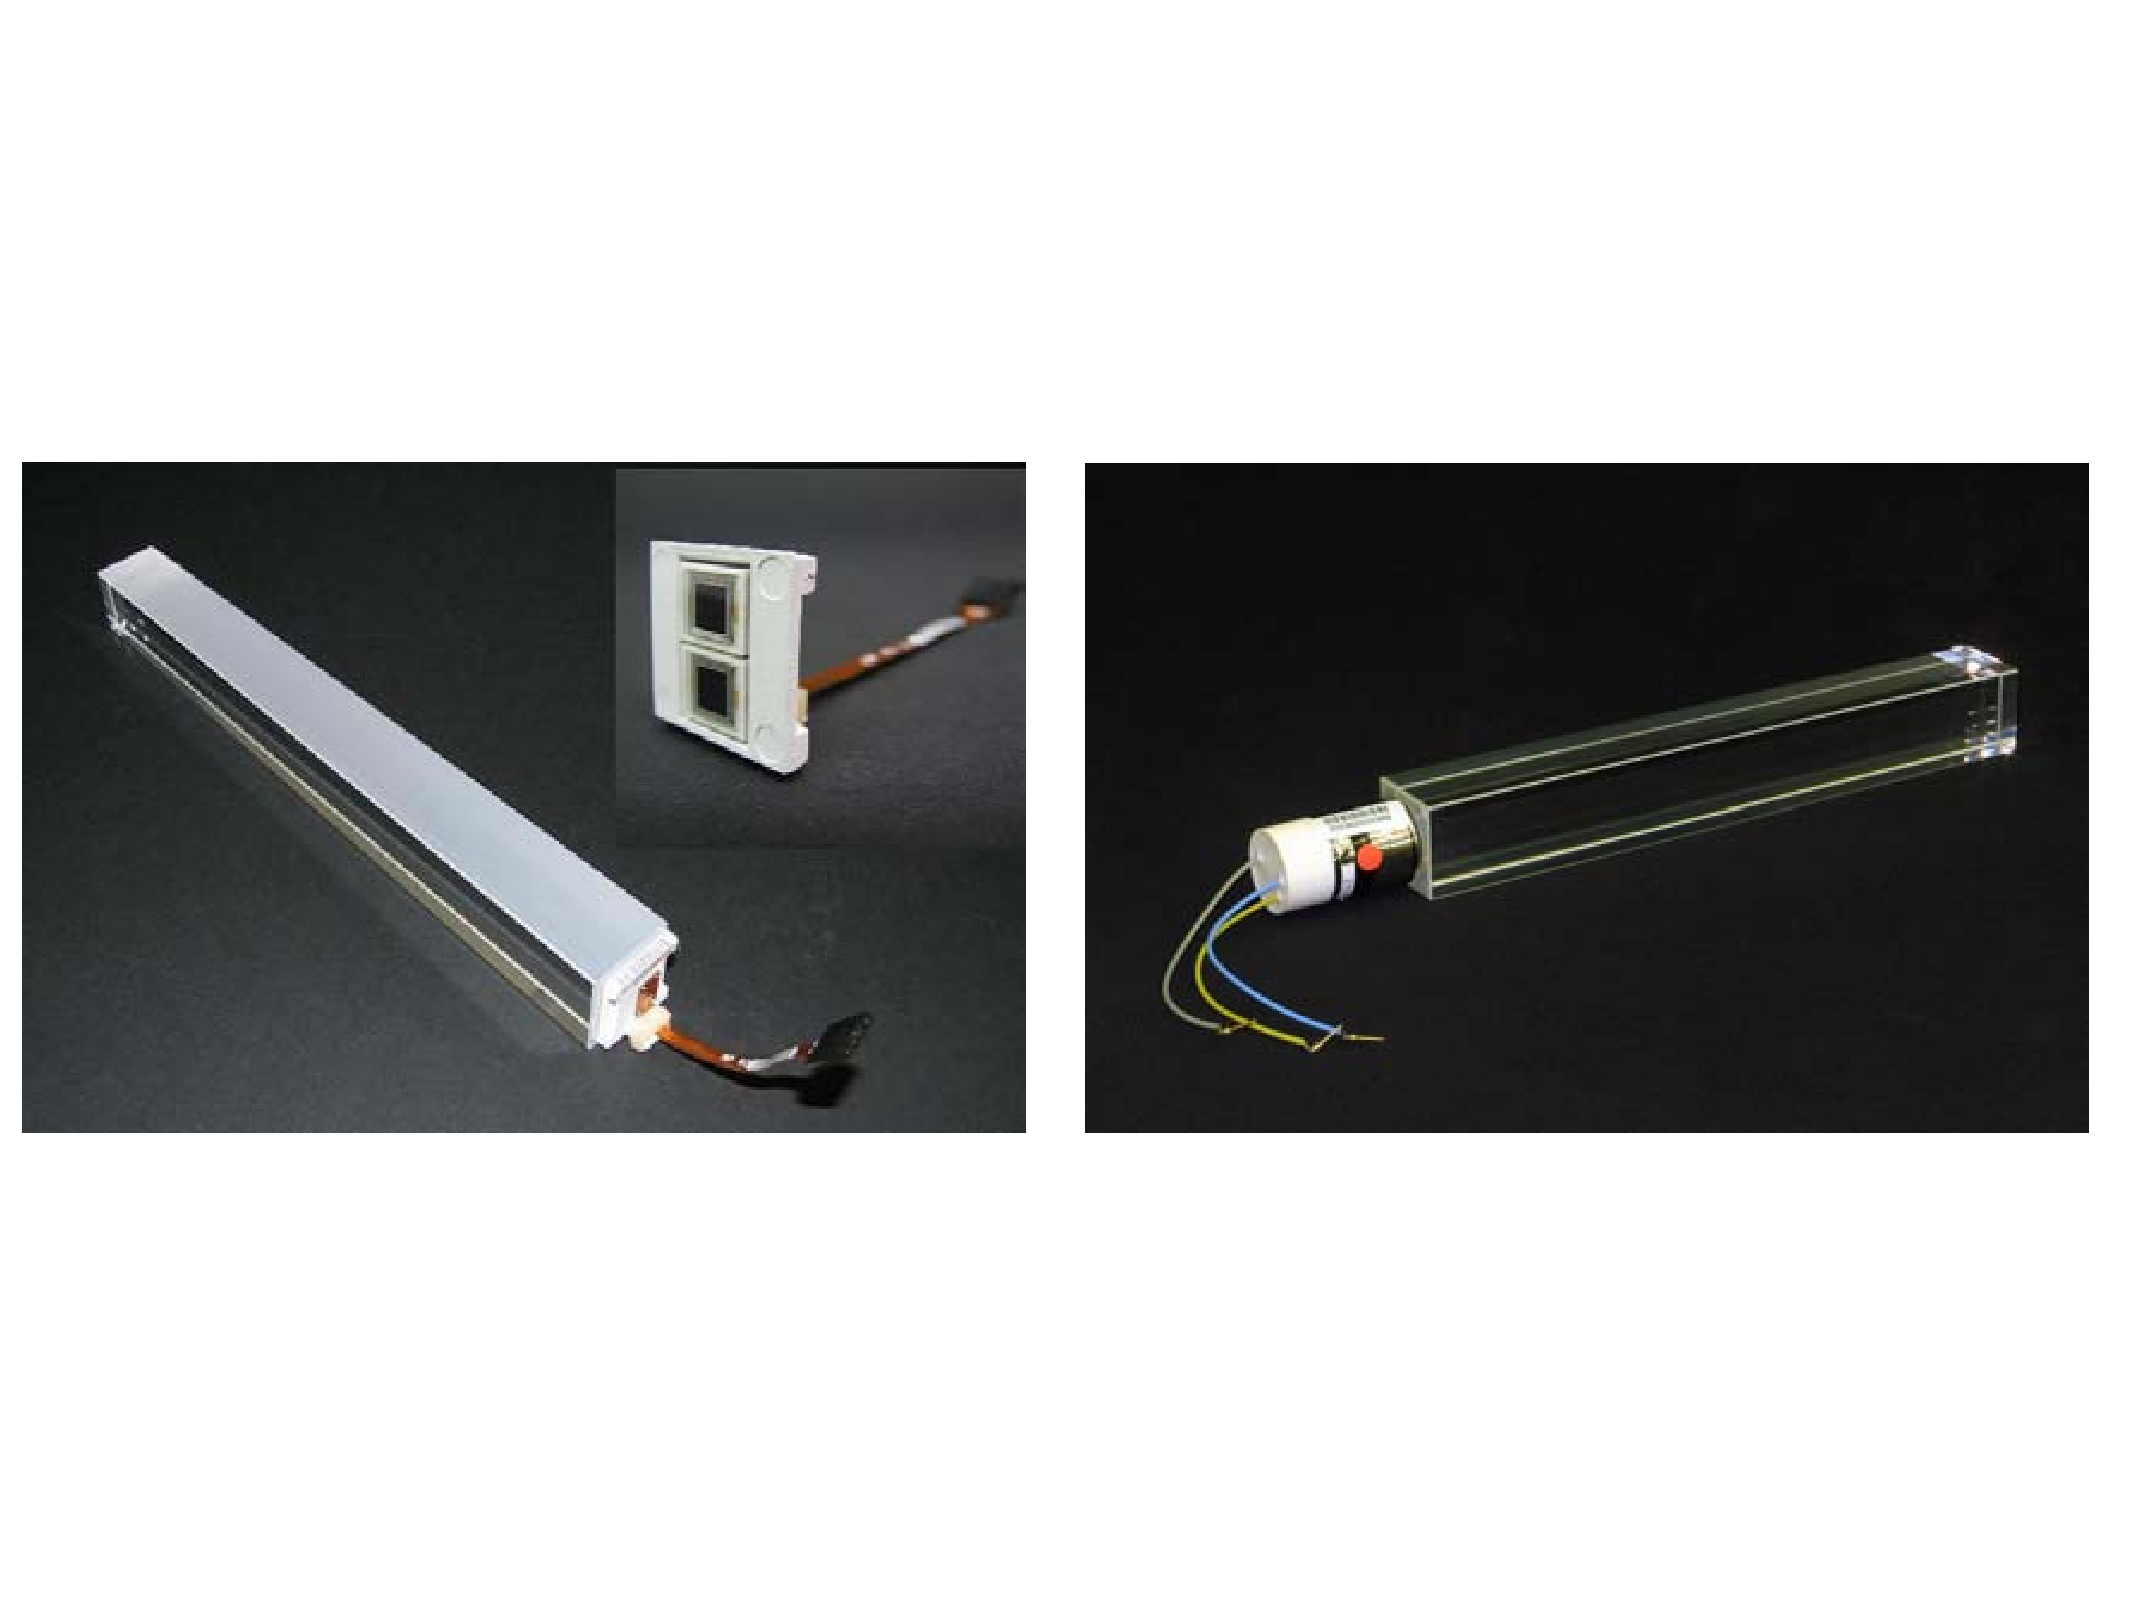
\includegraphics[width=0.99\textwidth]{CMS_DetectorFigures/EcalCrytals.pdf}
\caption{The  PbWO$_{4}$ crystal of the CMS ECAL, (left) a EB crystal
  instrumented with an APD and (right) a EE crystal instrumented with a VPT.\label{fig:ECALcrystals}}
\end{figure}
\begin{figure}
 \centering
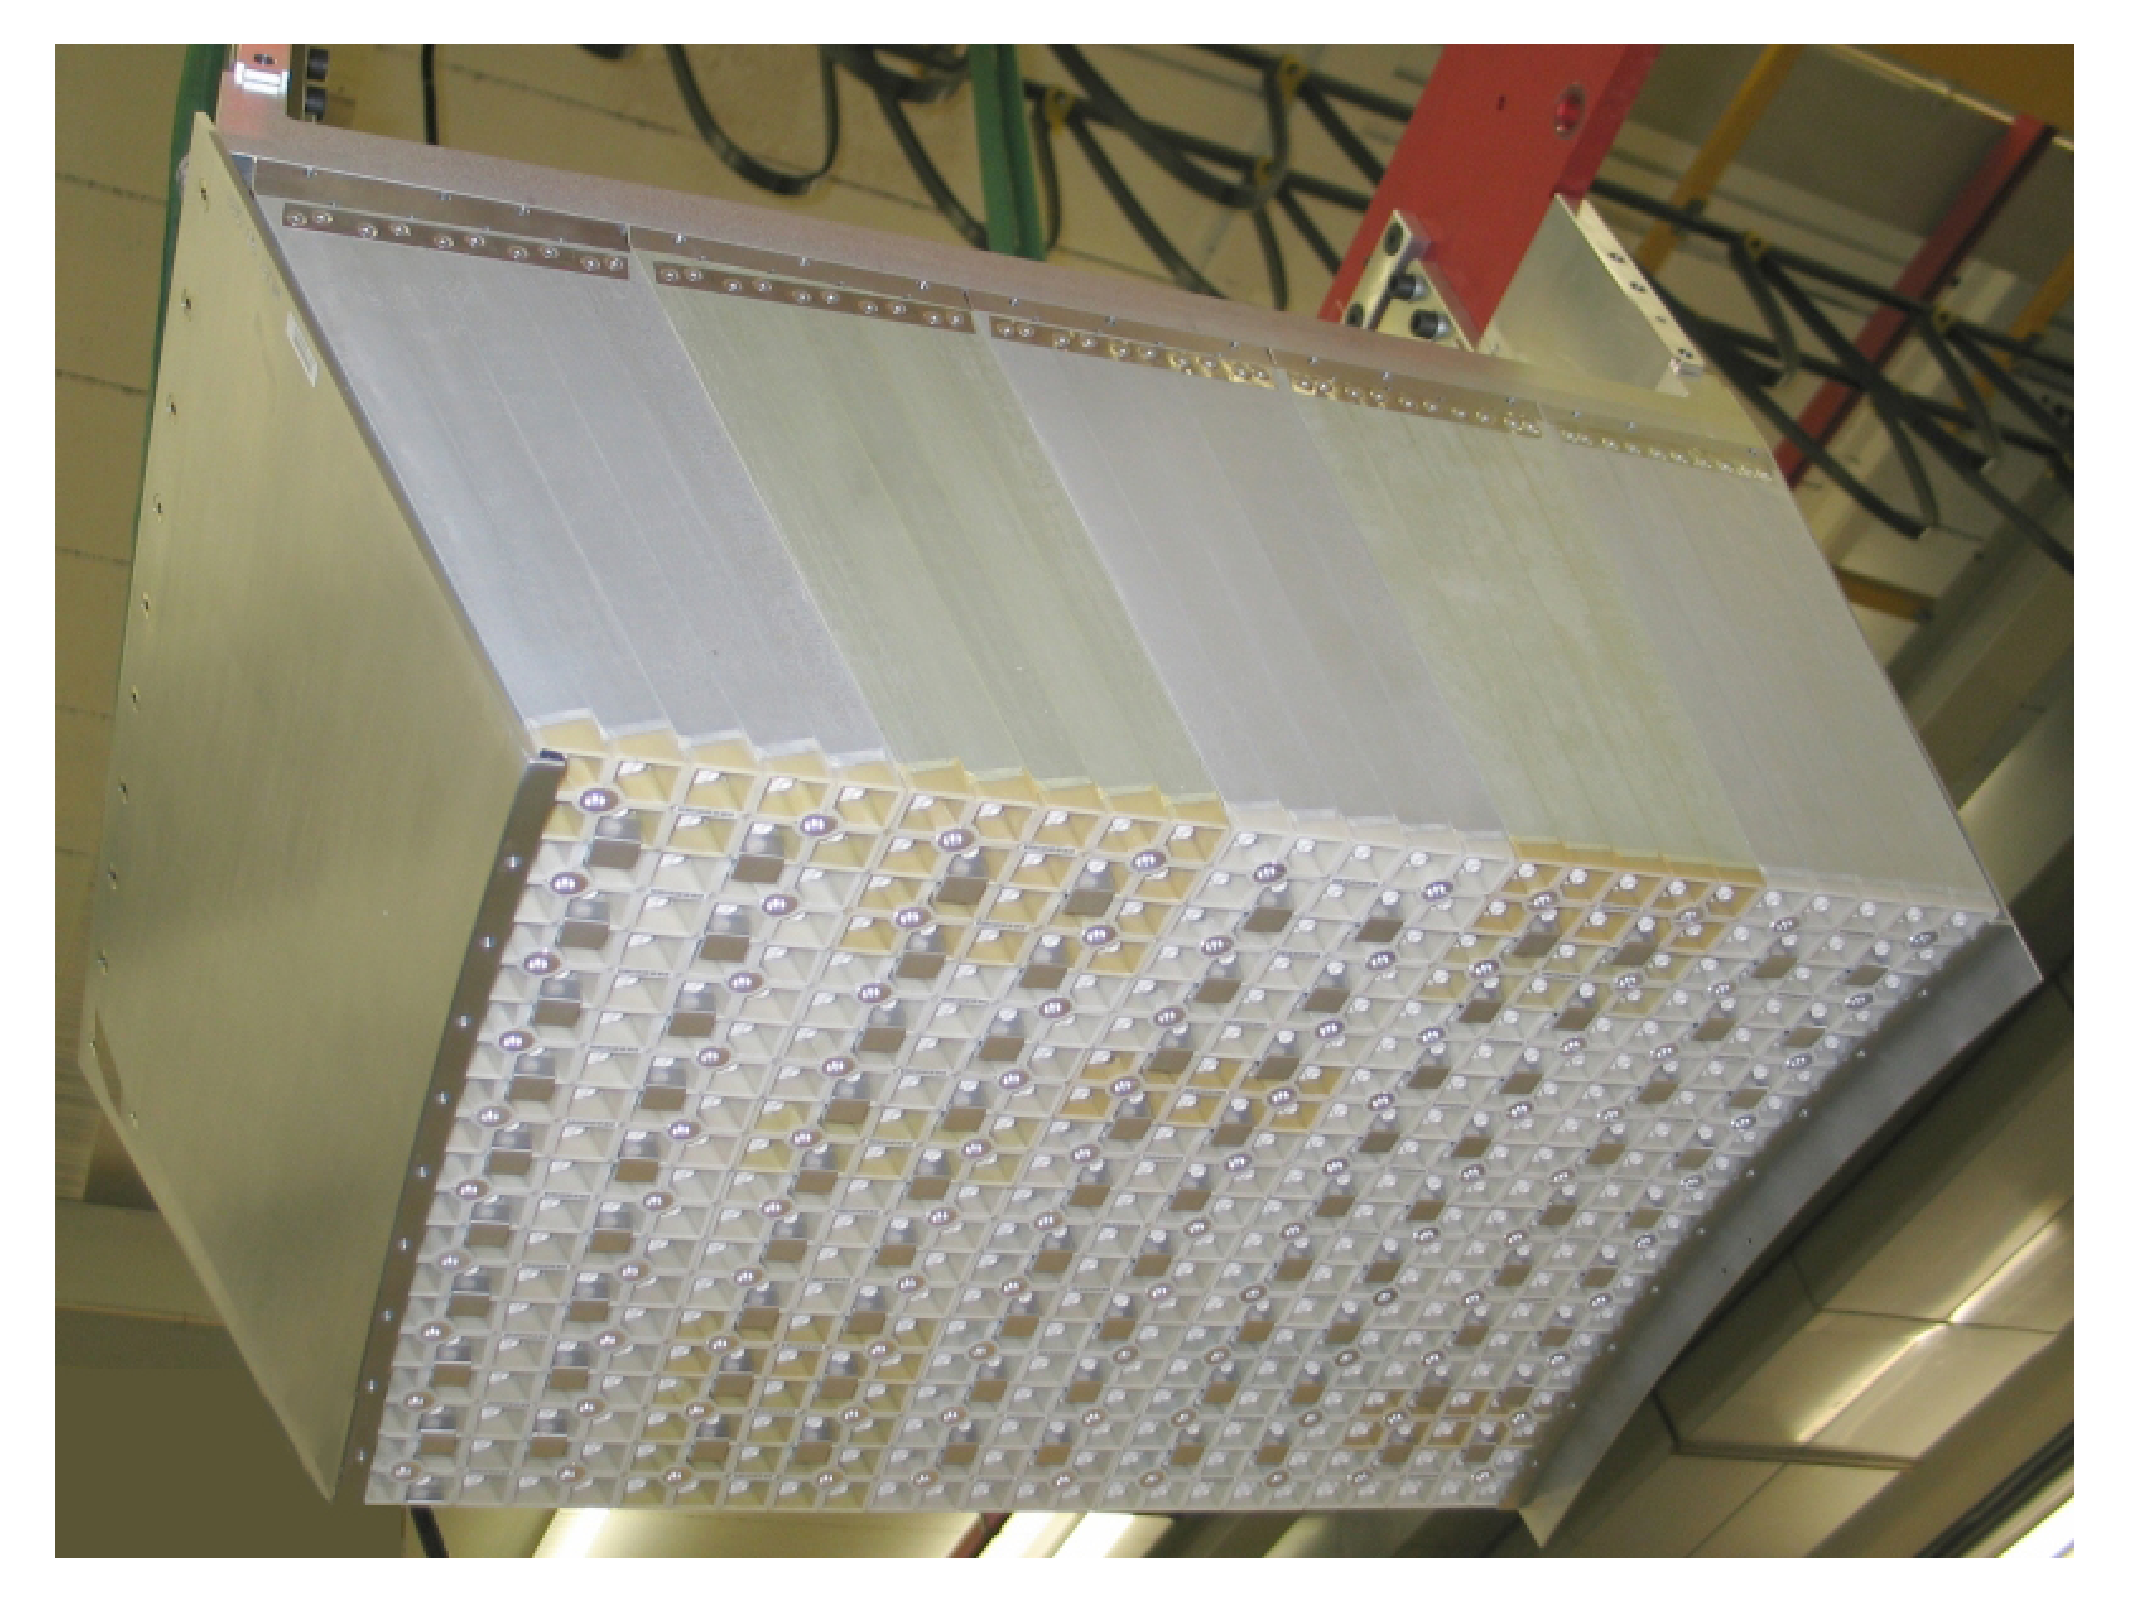
\includegraphics[width=0.99\textwidth]{CMS_DetectorFigures/ECALEB_Module.pdf}
\caption{A photograph of a EB module instrumented with crystals.\label{fig:ECALEB_module}}
\end{figure}
\begin{figure}
 \centering
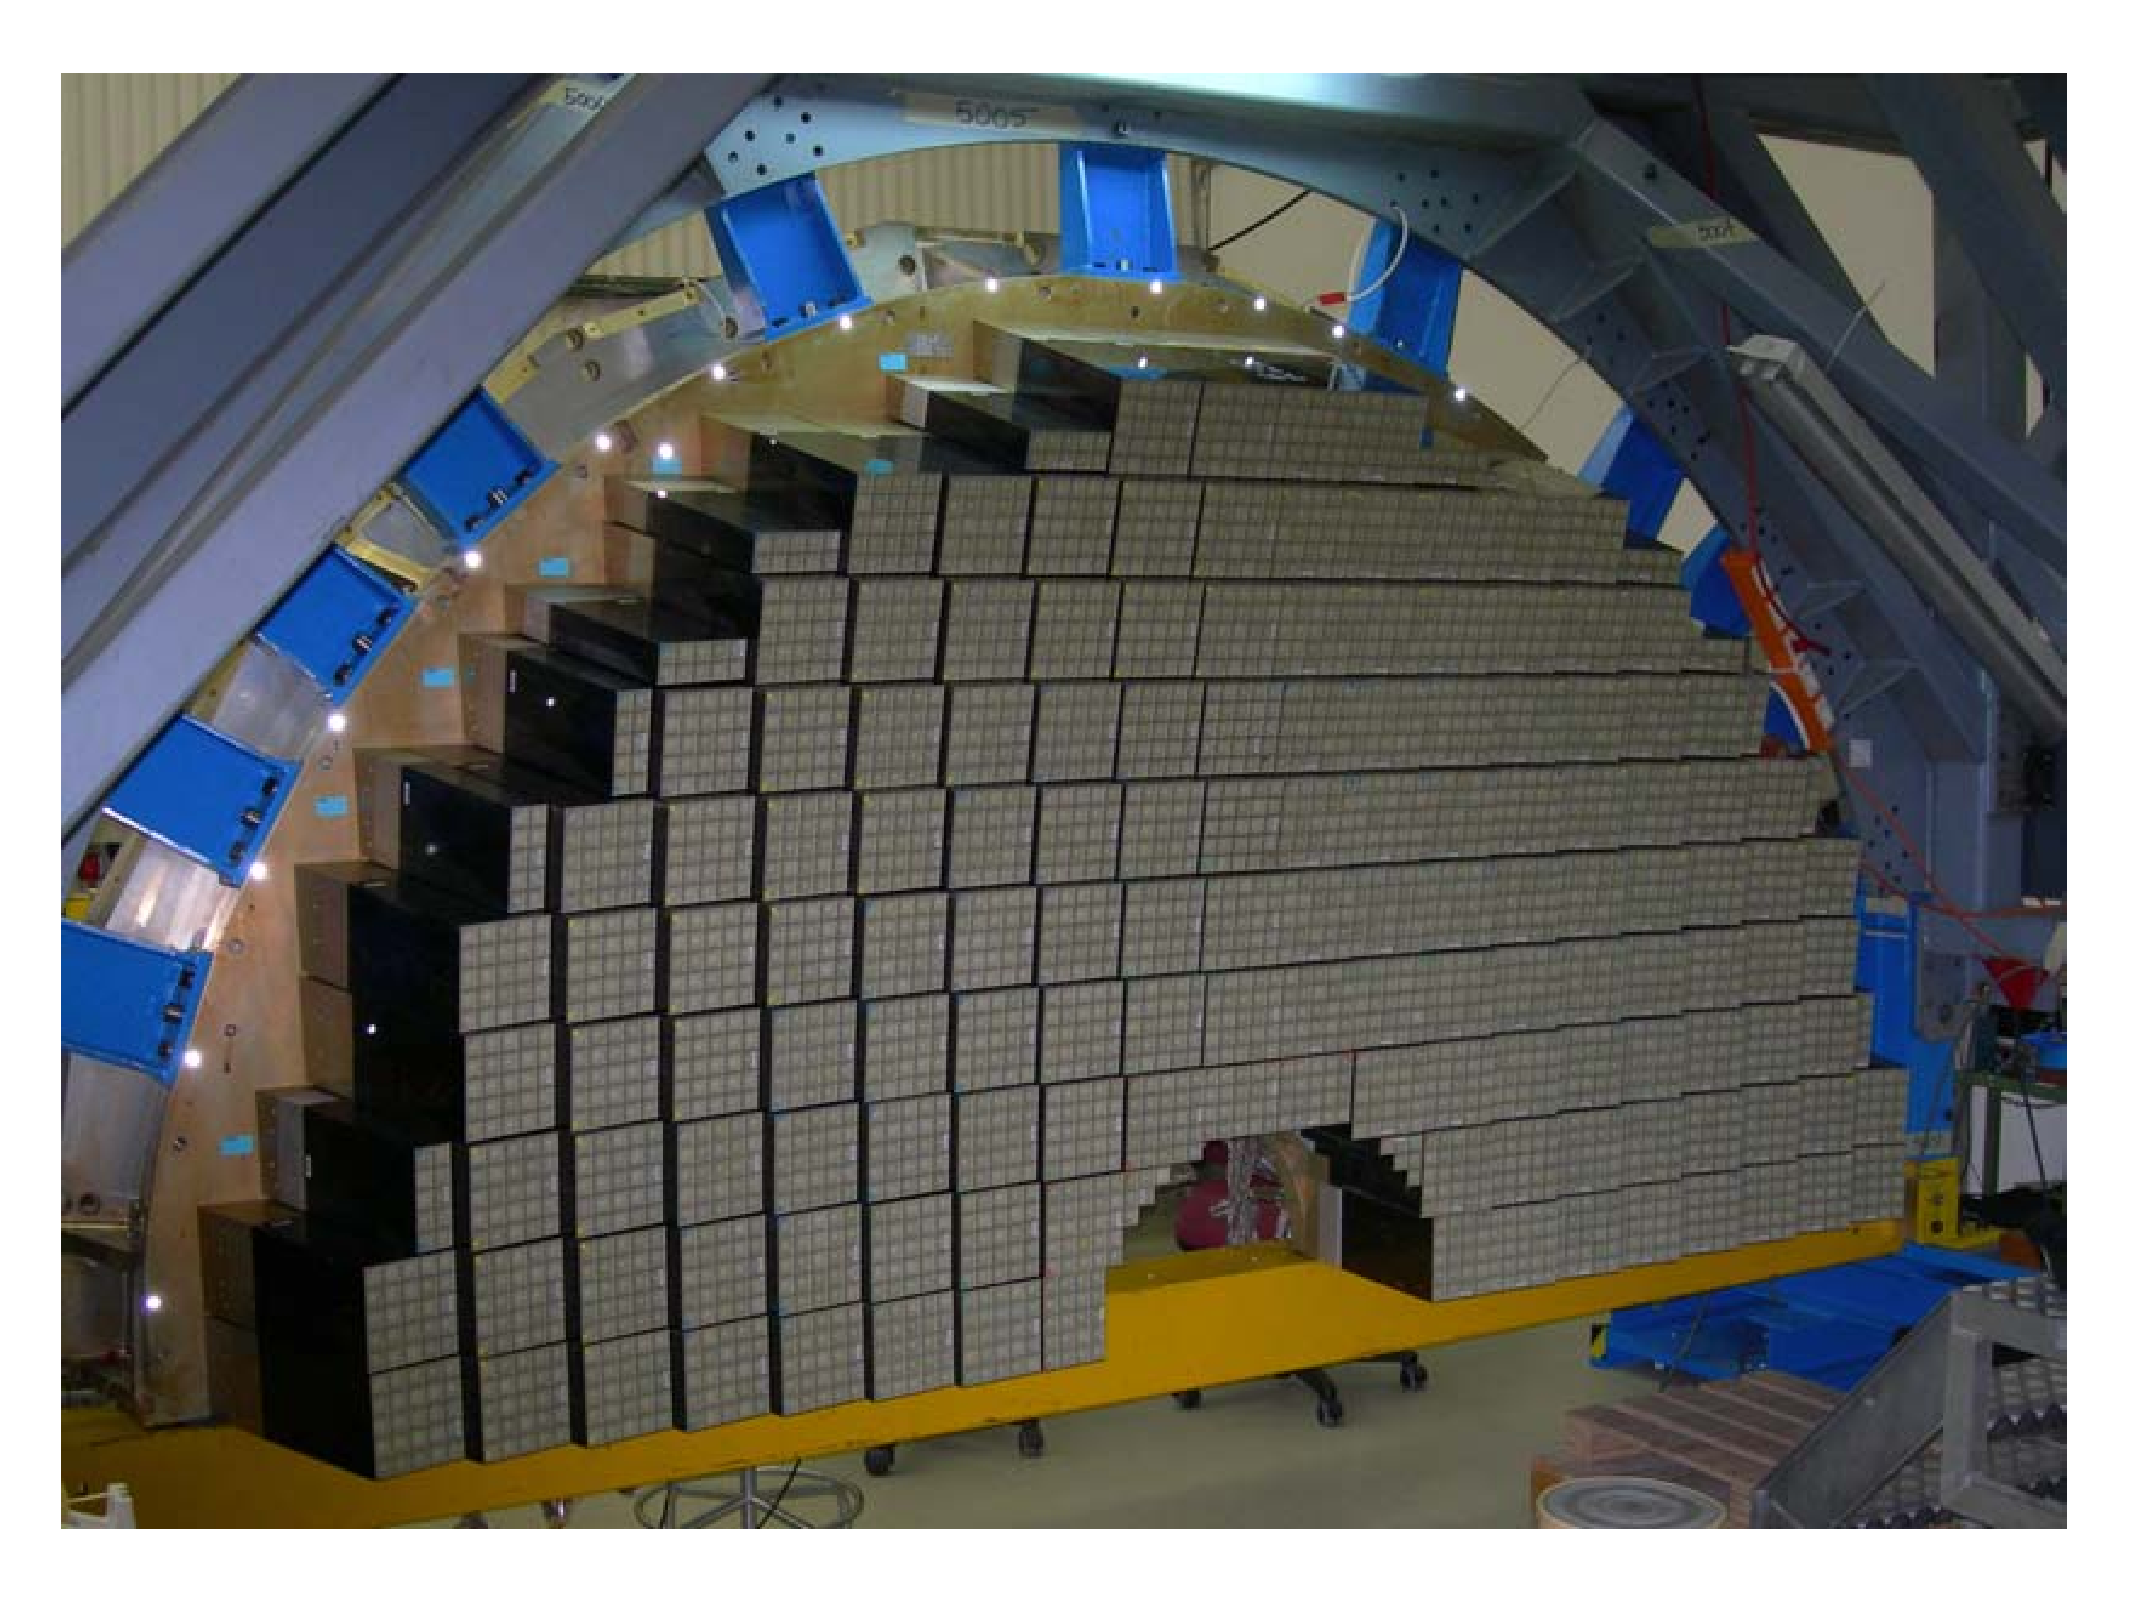
\includegraphics[width=0.99\textwidth]{CMS_DetectorFigures/ECALEE_Module.pdf}
\caption{A photograph of a EE Dee instrumented with crystals.\label{fig:ECALEE_module}}
\end{figure}
\subsection{ECAL Perfomance}

The EB has been extensively tested using electron beams, in this test
beam setup -- with no magnetic field or material in front -- the
energy resolution has been measured to be:
\begin{equation}\label{eq:ecalRes}
\frac{\sigma_{E}}{E} = \frac{2.8\%}{\sqrt{E(\GeV)}} \oplus
\frac{12\%}{E(\GeV)} \oplus 0.3\%,
\end{equation}

where E is the electron beam energy in units of \GeV. The terms in the
right-hand side of the Eq.~\ref{eq:ecalRes} are the so called
stochastic, noise, and constant terms. The first is due to the
fluctuations related to the development of the electromagnetic shower
inside the calorimenter crystals, the second is dues to electronic
noise of the readout chain, and the last is related to the
instrumental effect such as non-linear response, radiation damage,
shower leakage among others.

The test beam ideal conditions clearly differ from those at the CMS
experiment and therefore in situ measurements of the performance of
the ECAL have been performed durin the data-taking period at 7 and
8\TeV. One key measurement is the trigger efficiency for
electron/photon (e/$\gamma$) candidates, the Level-1 trigger was
operated with a threshold of $E_{T}$ = 20\GeV (provided by 5$\times$5
crystals) in 2012 and found to be above 99\% efficienct for $E_{T}$ >
40\GeV, thus enabling a fully efficienct H$\rightarrow\gamma\gamma$
search.

The e/$\gamma$ energy measurement depends upon the correct
reconstruction of electromagnetic showers in the ECAL. Some e/$\gamma$
candidates interact -- by bremsstrahlung or photon conversion -- with
the silicon tracker  prior reaching the ECAL or their trajectories are
modified due to the 3.8 T magnetic field causing the showers to spread
on the azhimutal direction and thus their energy is shared by multiple
crystals. In order to account for these effect and ensure a more
accurate e/$\gamma$ reconstruction a dynamic clustering algorithim is
used to merge clusters of energy deposited that belong to the same
electromagnetic shower into the so-called \textit{superclusters}
(SCs). Once the SC is formed, the e/$\gamma$ candidate energy
($E_{e/\gamma}$) is reconstructed using the following expression:

\begin{equation}
\label{eq:ecalE}
E_{e/\gamma} = F_{e/\gamma}\cdot \big(G\cdot\sum S_{i}(t)C_{i}A_{i} + E_{\mathrm{ES}}\big)
\end{equation}
 
where $F_{e/\gamma}$ is a correction accounting for the imperfect
clustering, material, and geometric efffect; $G$ is the ADC-to-\GeV
conversion; $S_{i}(t)$ is the time-dependent correction to account for
the response variations of the $i$-th crystal; $C_{i}$ is the
inter-calibration coefficient of the $i$-th crystal; $A_{i}$ is the
amplitude of the $i$-th crystal in ADC counts; finally,
$E_{\mathrm{ES}}$ is the pre-shower energy -- only relevant for
e/$\gamma$s in the EE. Figure~\ref{fig:ECAL_clusterE} shows the effect
of the clustering process and the application of the $F_{e/\gamma}$
correction by comparing the invariant mass of $e^{+}e^{-}$ pairs
coming from a Z boson with respect to the usage of the simple fixed
5$\times$5 cluster energy.

\begin{figure}
 \centering
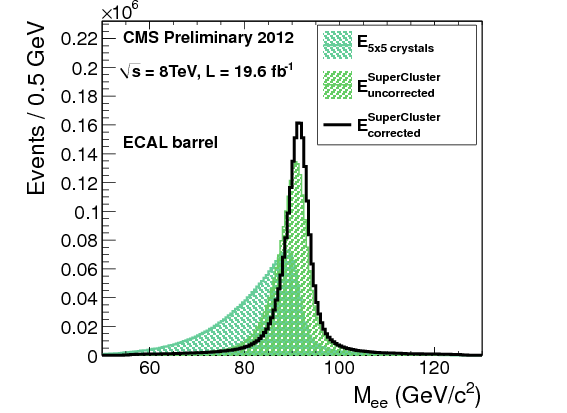
\includegraphics[width=0.49\textwidth]{CMS_DetectorFigures/E_corr-EB.png}
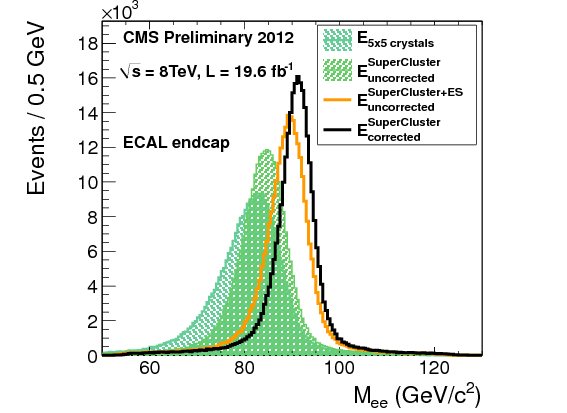
\includegraphics[width=0.49\textwidth]{CMS_DetectorFigures/E_corr-EE.png}
\caption{The reconstructed Z invariant mass from $e^{+}e^{-}$
  decays. The left and right panels show the reconstructed invariant mass for
  the EB and EE, repectively, with different algorithms to reconstructed electron energies.\label{fig:ECAL_clusterE}}
\end{figure}

The inter-calibration coefficient is responsible for correcting the
channel-to-channel variation in response. The main sources for such
variations are the crystal light yield variations ( up to $\sim$ 15\%)
and the spread on the gain of the photodetectors ( up to $\sim$
25\%). An inter-calibration is carrried out in situ by methods that
explote the time- and $\phi$-invariance of the energy flow in the
crystals at a given $\eta$ in minimum-bias events, as well as the
$\pi^{0}/eta$ mass constraint to the photons pair from its decay, and
the momentum constraint of isolated electrons from W and Z boson
decays. The precision of these methods as a function of $\eta$ is
shown in Figure~\ref{fig:ECAL_ICPrecision}. The invariant mass of
diphotons consistent with a $\pi^{0}$ and $\eta$ used in the
inter-calibration is shown in the left and right panels of
Figure~\ref{fig:ECAL_pizero}, respectively.

\begin{figure}
 \centering
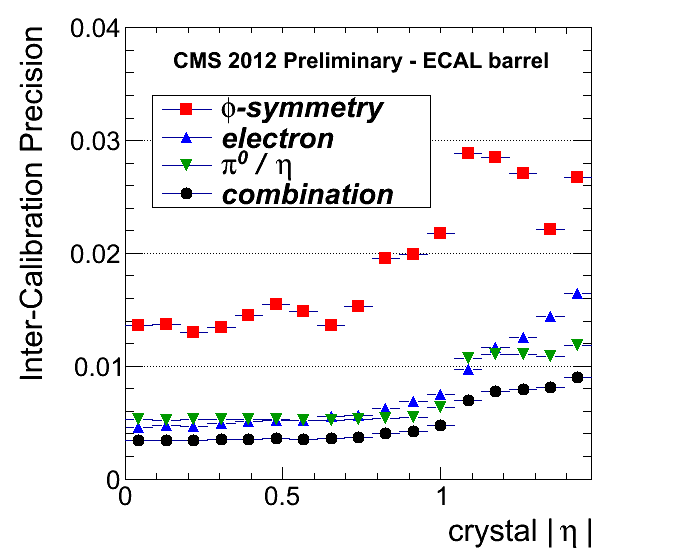
\includegraphics[width=0.49\textwidth]{CMS_DetectorFigures/2012EBprecWithCombV3.png}
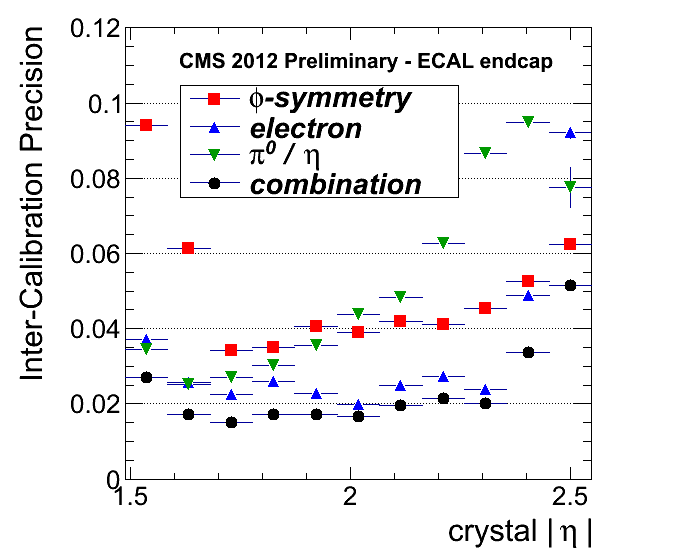
\includegraphics[width=0.49\textwidth]{CMS_DetectorFigures/2012EEprecWithCombV3.png}
\caption{The reconstructed Z invariant mass from $e^{+}e^{-}$
  decays. The left and right panels show the reconstructed invariant mass for
  the EB and EE, repectively, with different algorithms to reconstructed electron energies.\label{fig:ECAL_ICPrecision}}
\end{figure}

\begin{figure}
 \centering
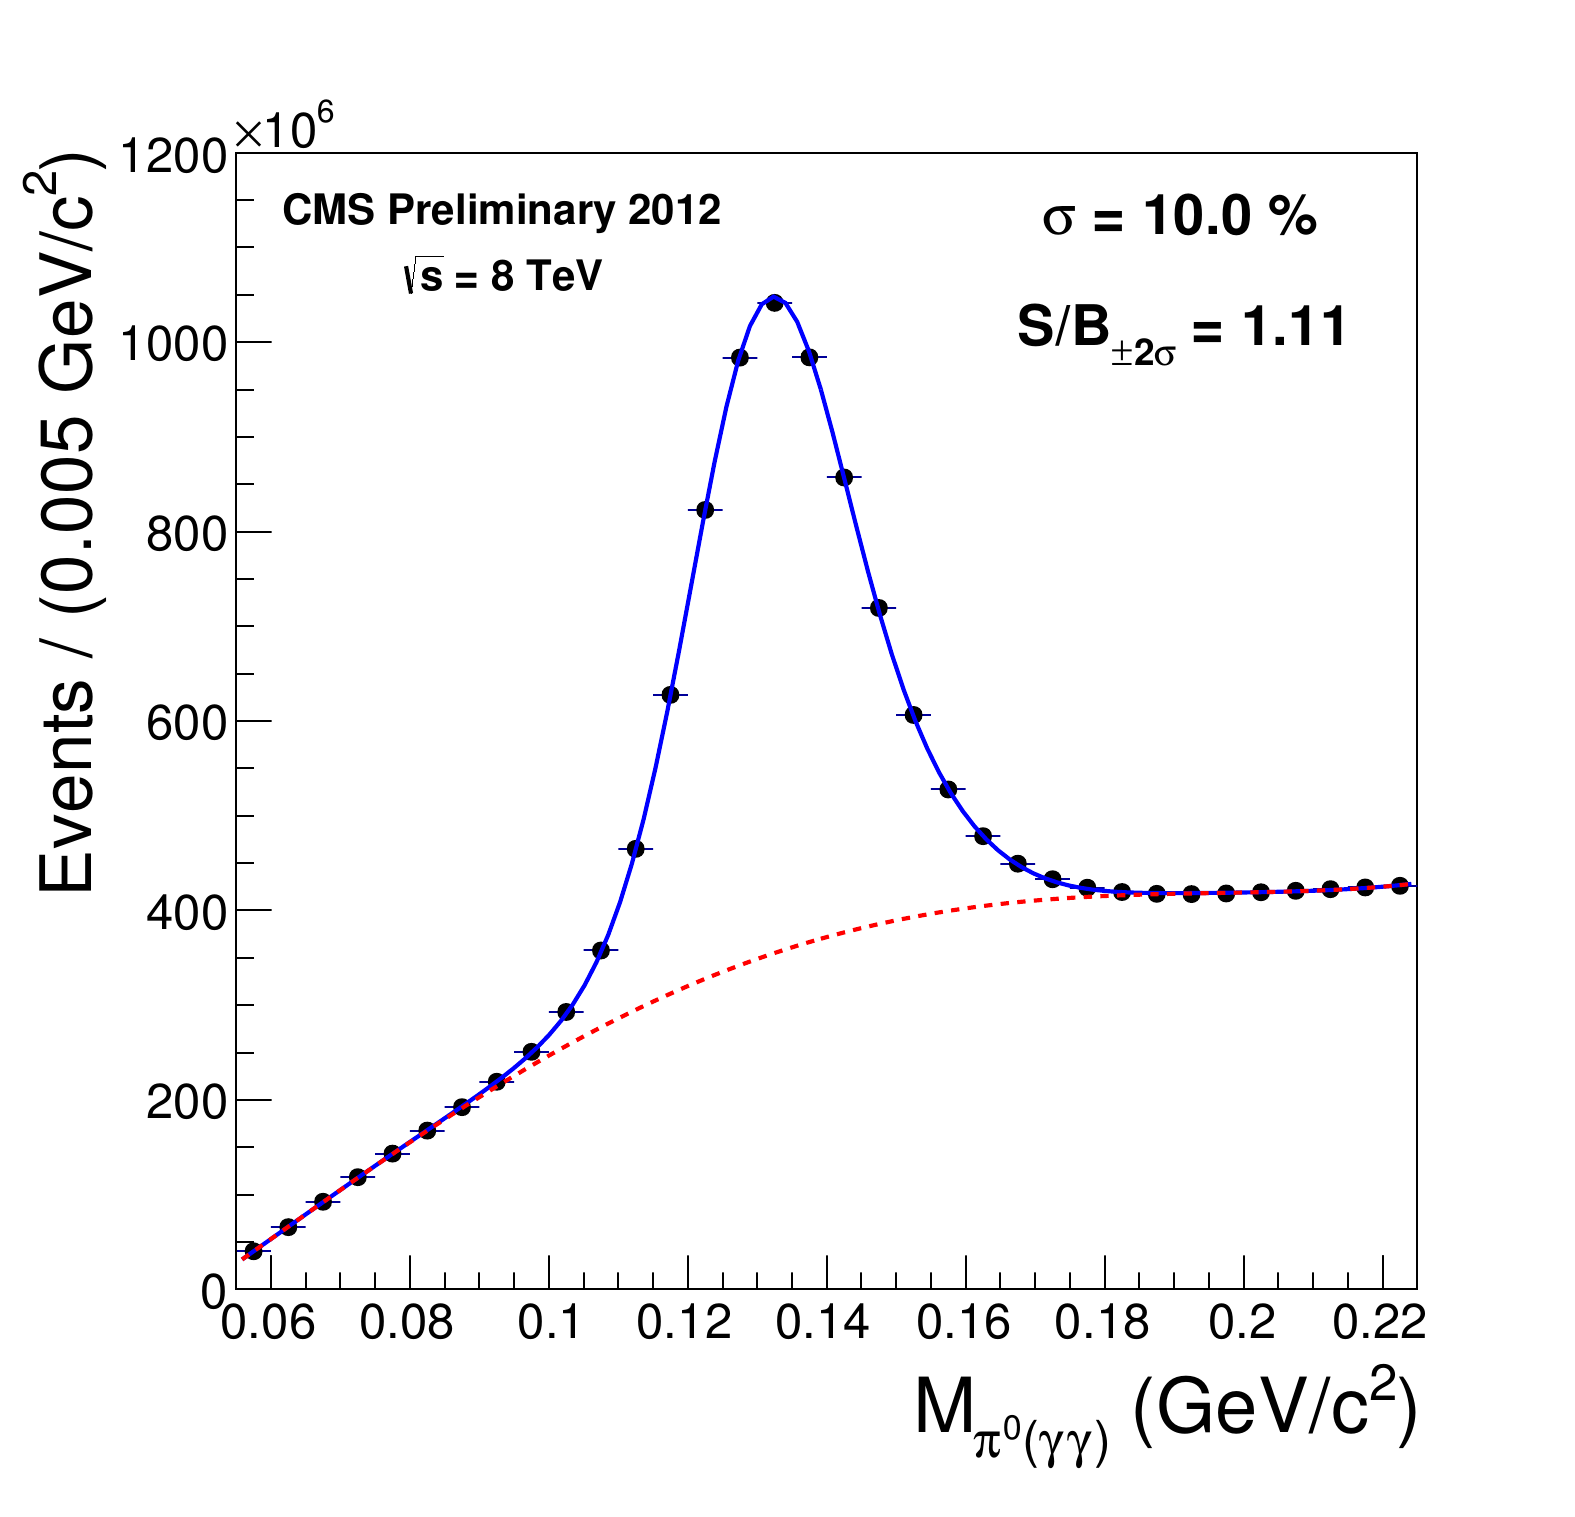
\includegraphics[width=0.49\textwidth]{CMS_DetectorFigures/EB_2012_pi0.png}
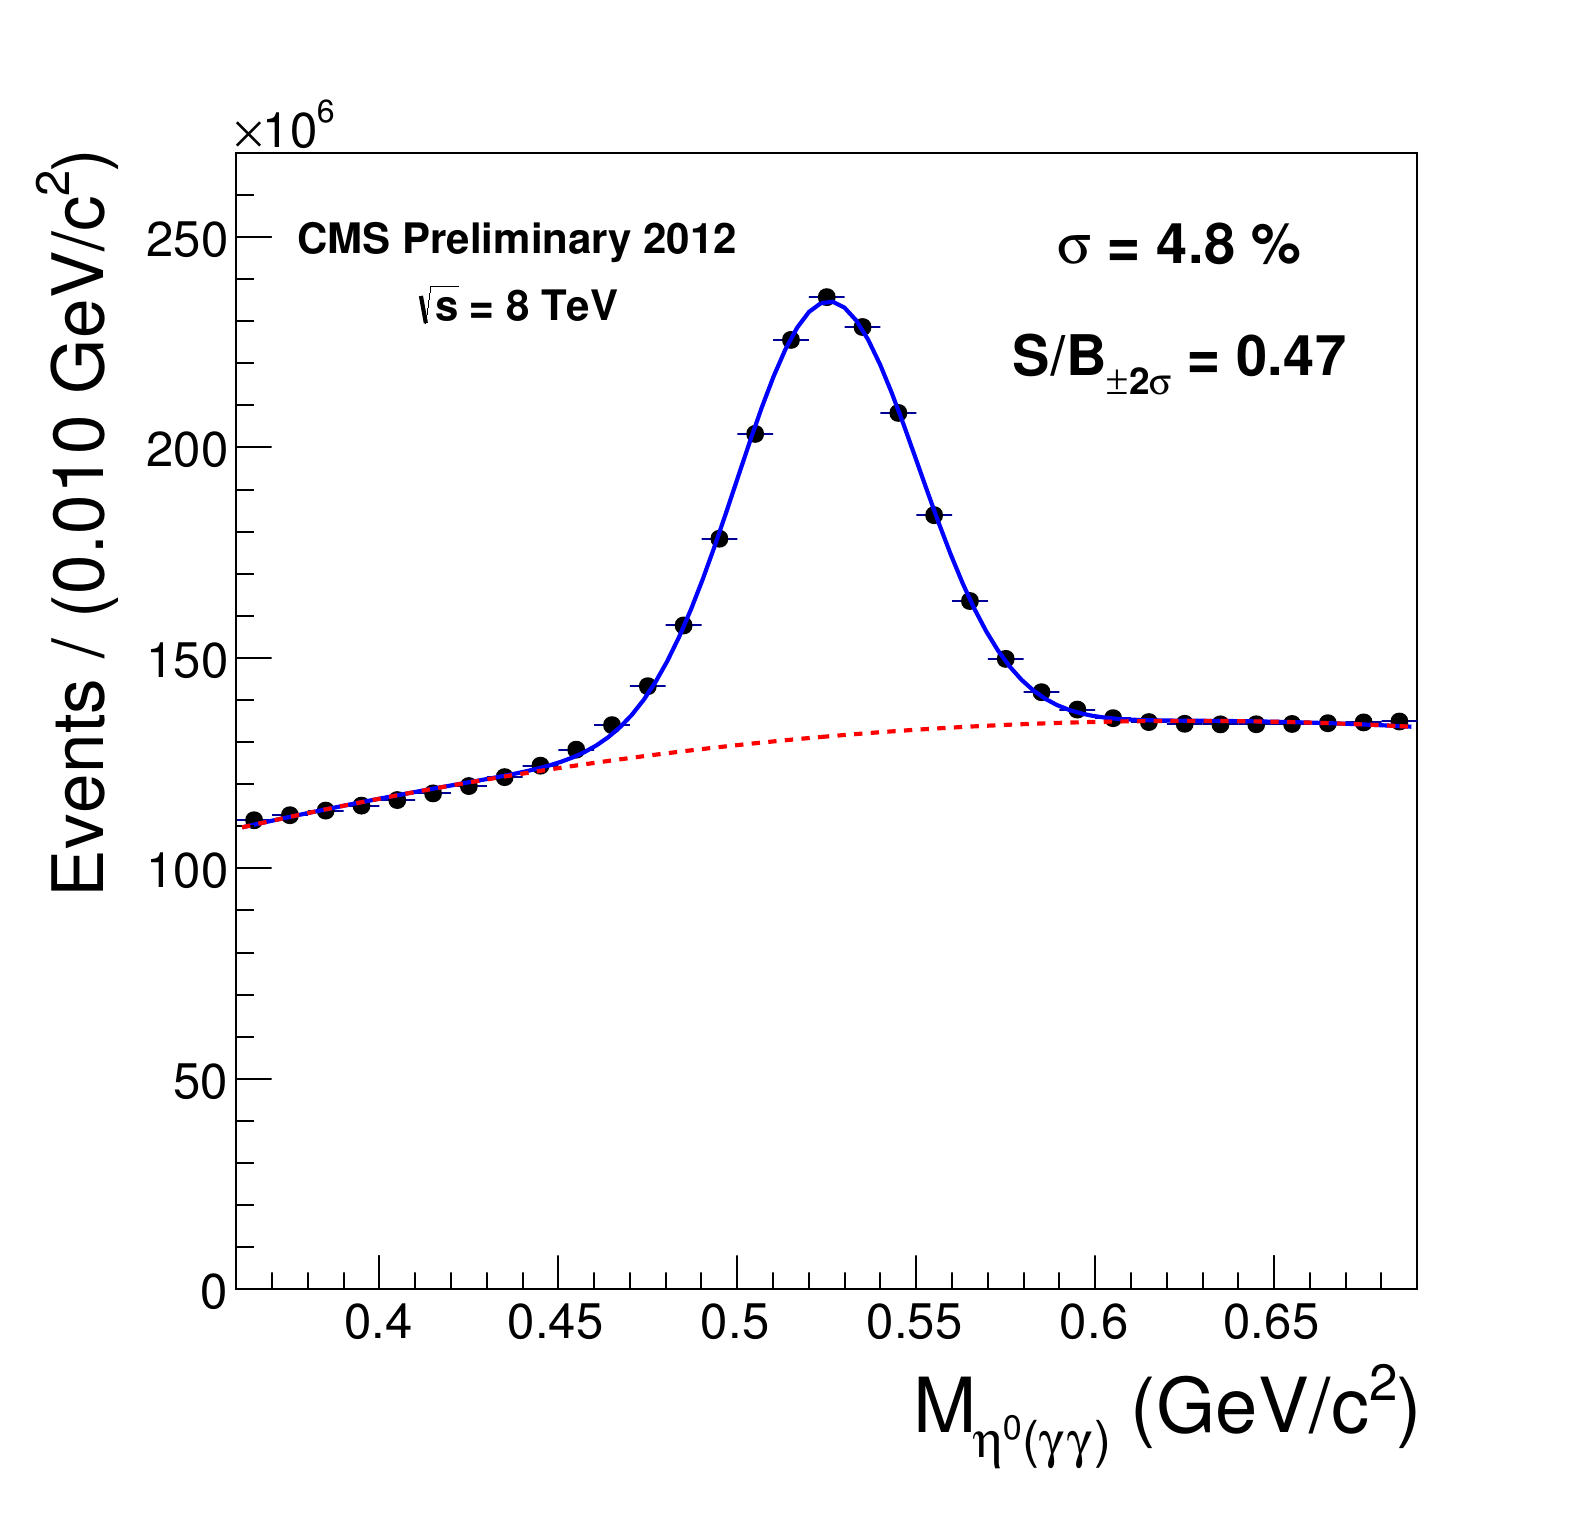
\includegraphics[width=0.49\textwidth]{CMS_DetectorFigures/EB_2012_eta0.png}
\caption{The reconstructed Z invariant mass from $e^{+}e^{-}$
  decays. The left and right panels show the reconstructed invariant mass for
  the EB and EE, repectively, with different algorithms to reconstructed electron energies.\label{fig:ECAL_pizero}}
\end{figure}
Another important ingredient to the precise measurement of the
electromagnetic shower energy is the time dependent corrections, at
CMS the ECAL crystals undergo changes in transparency due to the
radiation received while collisions occur, while  during downtime the
transparency is recovered. In order to correct for the transparency
changes a laser monitoring system is installed and run every $\sim$40
minutes. Laser light ($\lambda = 440$ nm) close to the emission peak of PbWO$_{4}$
is impinge into all the crystals, thus, tracking their response
variations. The variations on transparency as a function of time for
different $\eta$ ranges is shown in
the left panel of Figure~\ref{fig:ECAL_Transparency1}, where it is observed that the
transparency variations are more severe at large pseudorapidities. The
validity of the laser monitoring (LM) correction is checked using
electrons from W decays. The stability of the LM correction is
estimated by the rms of the $E/p$ ratio in these events and found to
be about 0.1\% and 0.3\% for the EB and EE, respectively. The right
panel of Figure~\ref{fig:ECAL_Transparency1} shown the LM correction
effect on electron from W events in the EE. The effect of the
inter-calibration and LM corrections is shown Figure~\ref{fig:ECAL_E_IC_LM}, where
the invariant mass of $e^{+}e^{-}$ pairs from Z decays is
reconstructed with and without such corrections being applied.
\begin{figure}
 \centering
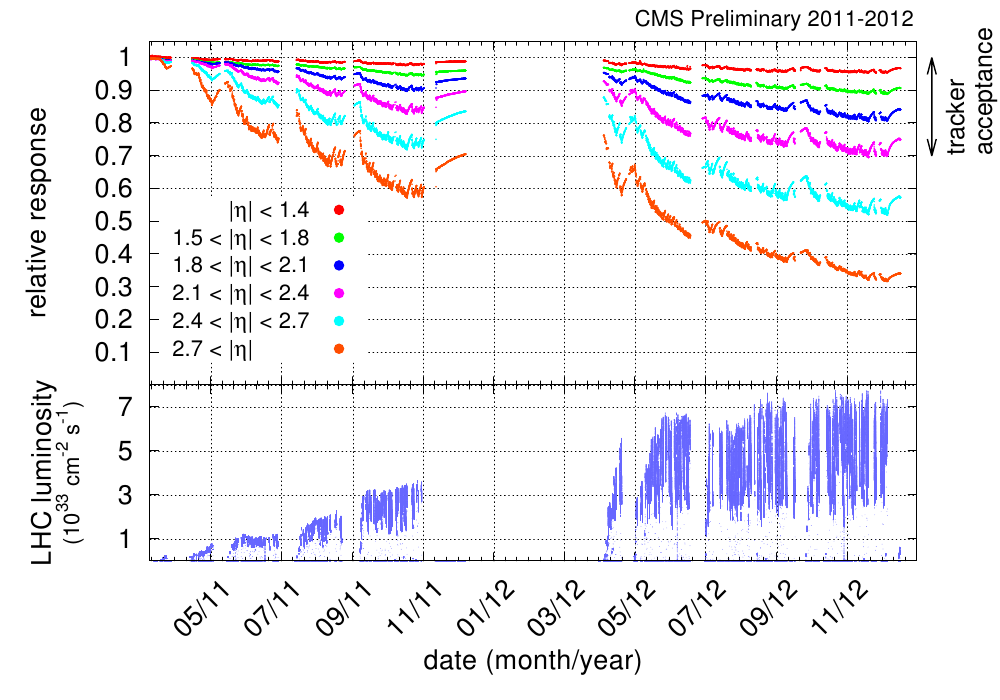
\includegraphics[width=0.99\textwidth]{CMS_DetectorFigures/histories_2011-2012.png}
\caption{The reconstructed Z invariant mass from $e^{+}e^{-}$
  decays. The left and right panels show the reconstructed invariant mass for
  the EB and EE, repectively, with different algorithms to reconstructed electron energies.\label{fig:ECAL_Transparency1}}
\end{figure}

\begin{figure}
 \centering
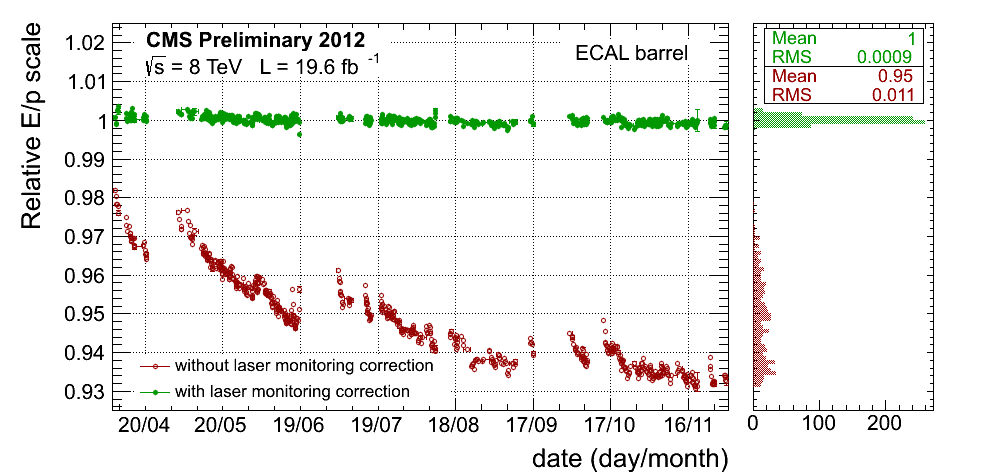
\includegraphics[width=0.99\textwidth]{CMS_DetectorFigures/approval_EB_Winter2013.png}
\caption{The reconstructed Z invariant mass from $e^{+}e^{-}$
  decays. The left and right panels show the reconstructed invariant mass for
  the EB and EE, repectively, with different algorithms to reconstructed electron energies.\label{fig:ECAL_response}}
\end{figure}

\begin{figure}
 \centering
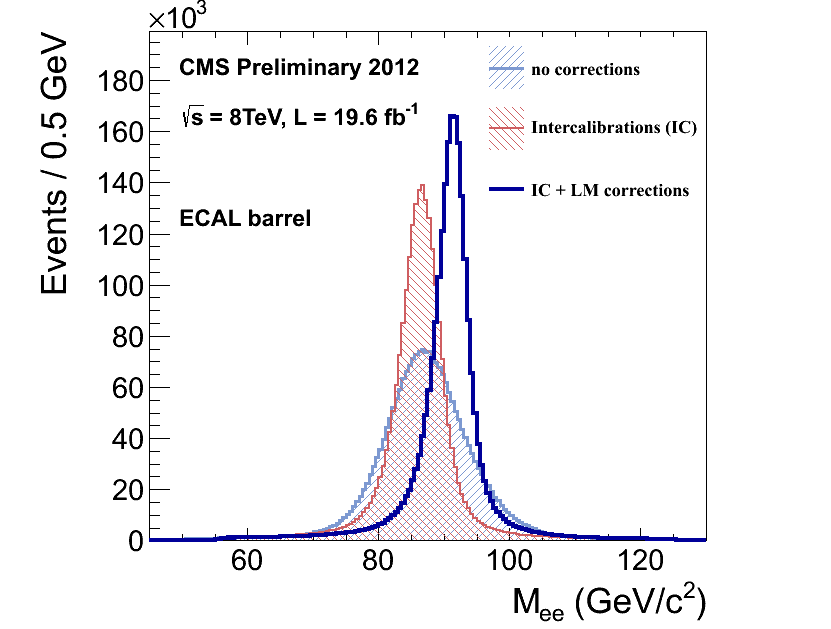
\includegraphics[width=0.49\textwidth]{CMS_DetectorFigures/noIC_noLaser-regrCorr_ele-EB.png}
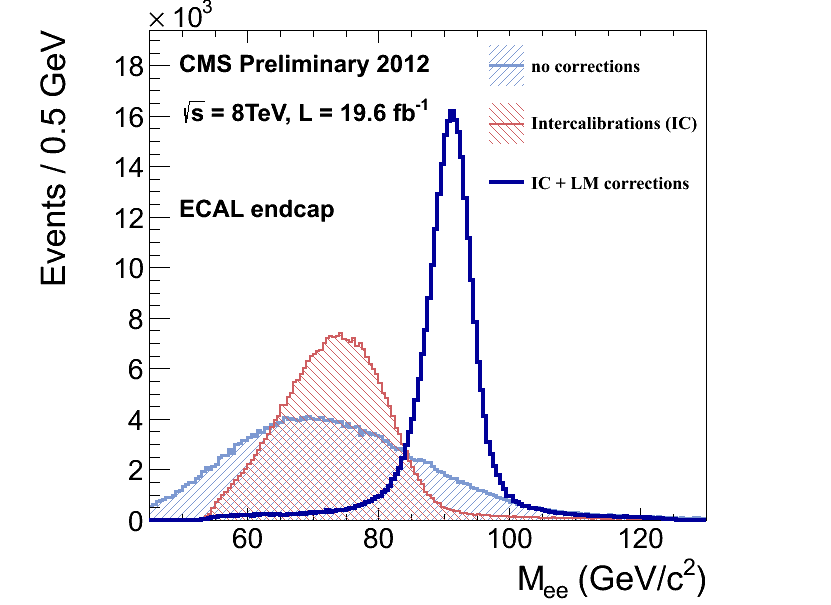
\includegraphics[width=0.49\textwidth]{CMS_DetectorFigures/propaganda_noIC_noLaser-regrCorr_ele-EE.png}
\caption{The reconstructed Z invariant mass from $e^{+}e^{-}$
  decays. The left and right panels show the reconstructed invariant mass for
  the EB and EE, repectively, with and without the IC and the LM corrections.\label{fig:ECAL_E_IC_LM}}
\end{figure}
 Finally, the overall energy resolution of the CMS ECAL has been measured
 and compared to simulation, this is shown in the right panel of
 Figure~\ref{fig:ECAL_Higgs}. The energy resolution is found to be
 between 1-2\% for $|\eta|<1$ and between 3-5\% in the EE, it is also
 observed that the simulation and measurement do not agree and that an
 extra constant term as a function of $\eta$ should be added to the
 simulation. The performance of the ECAL can also be observed in the
 width of the invariant mass of the Higgs boson, this is shown in the
 left panel of Figure~\ref{fig:ECAL_Higgs}, where a $\sigma_{eff}$ =
 1.36\GeV is observed.
\begin{figure}
 \centering
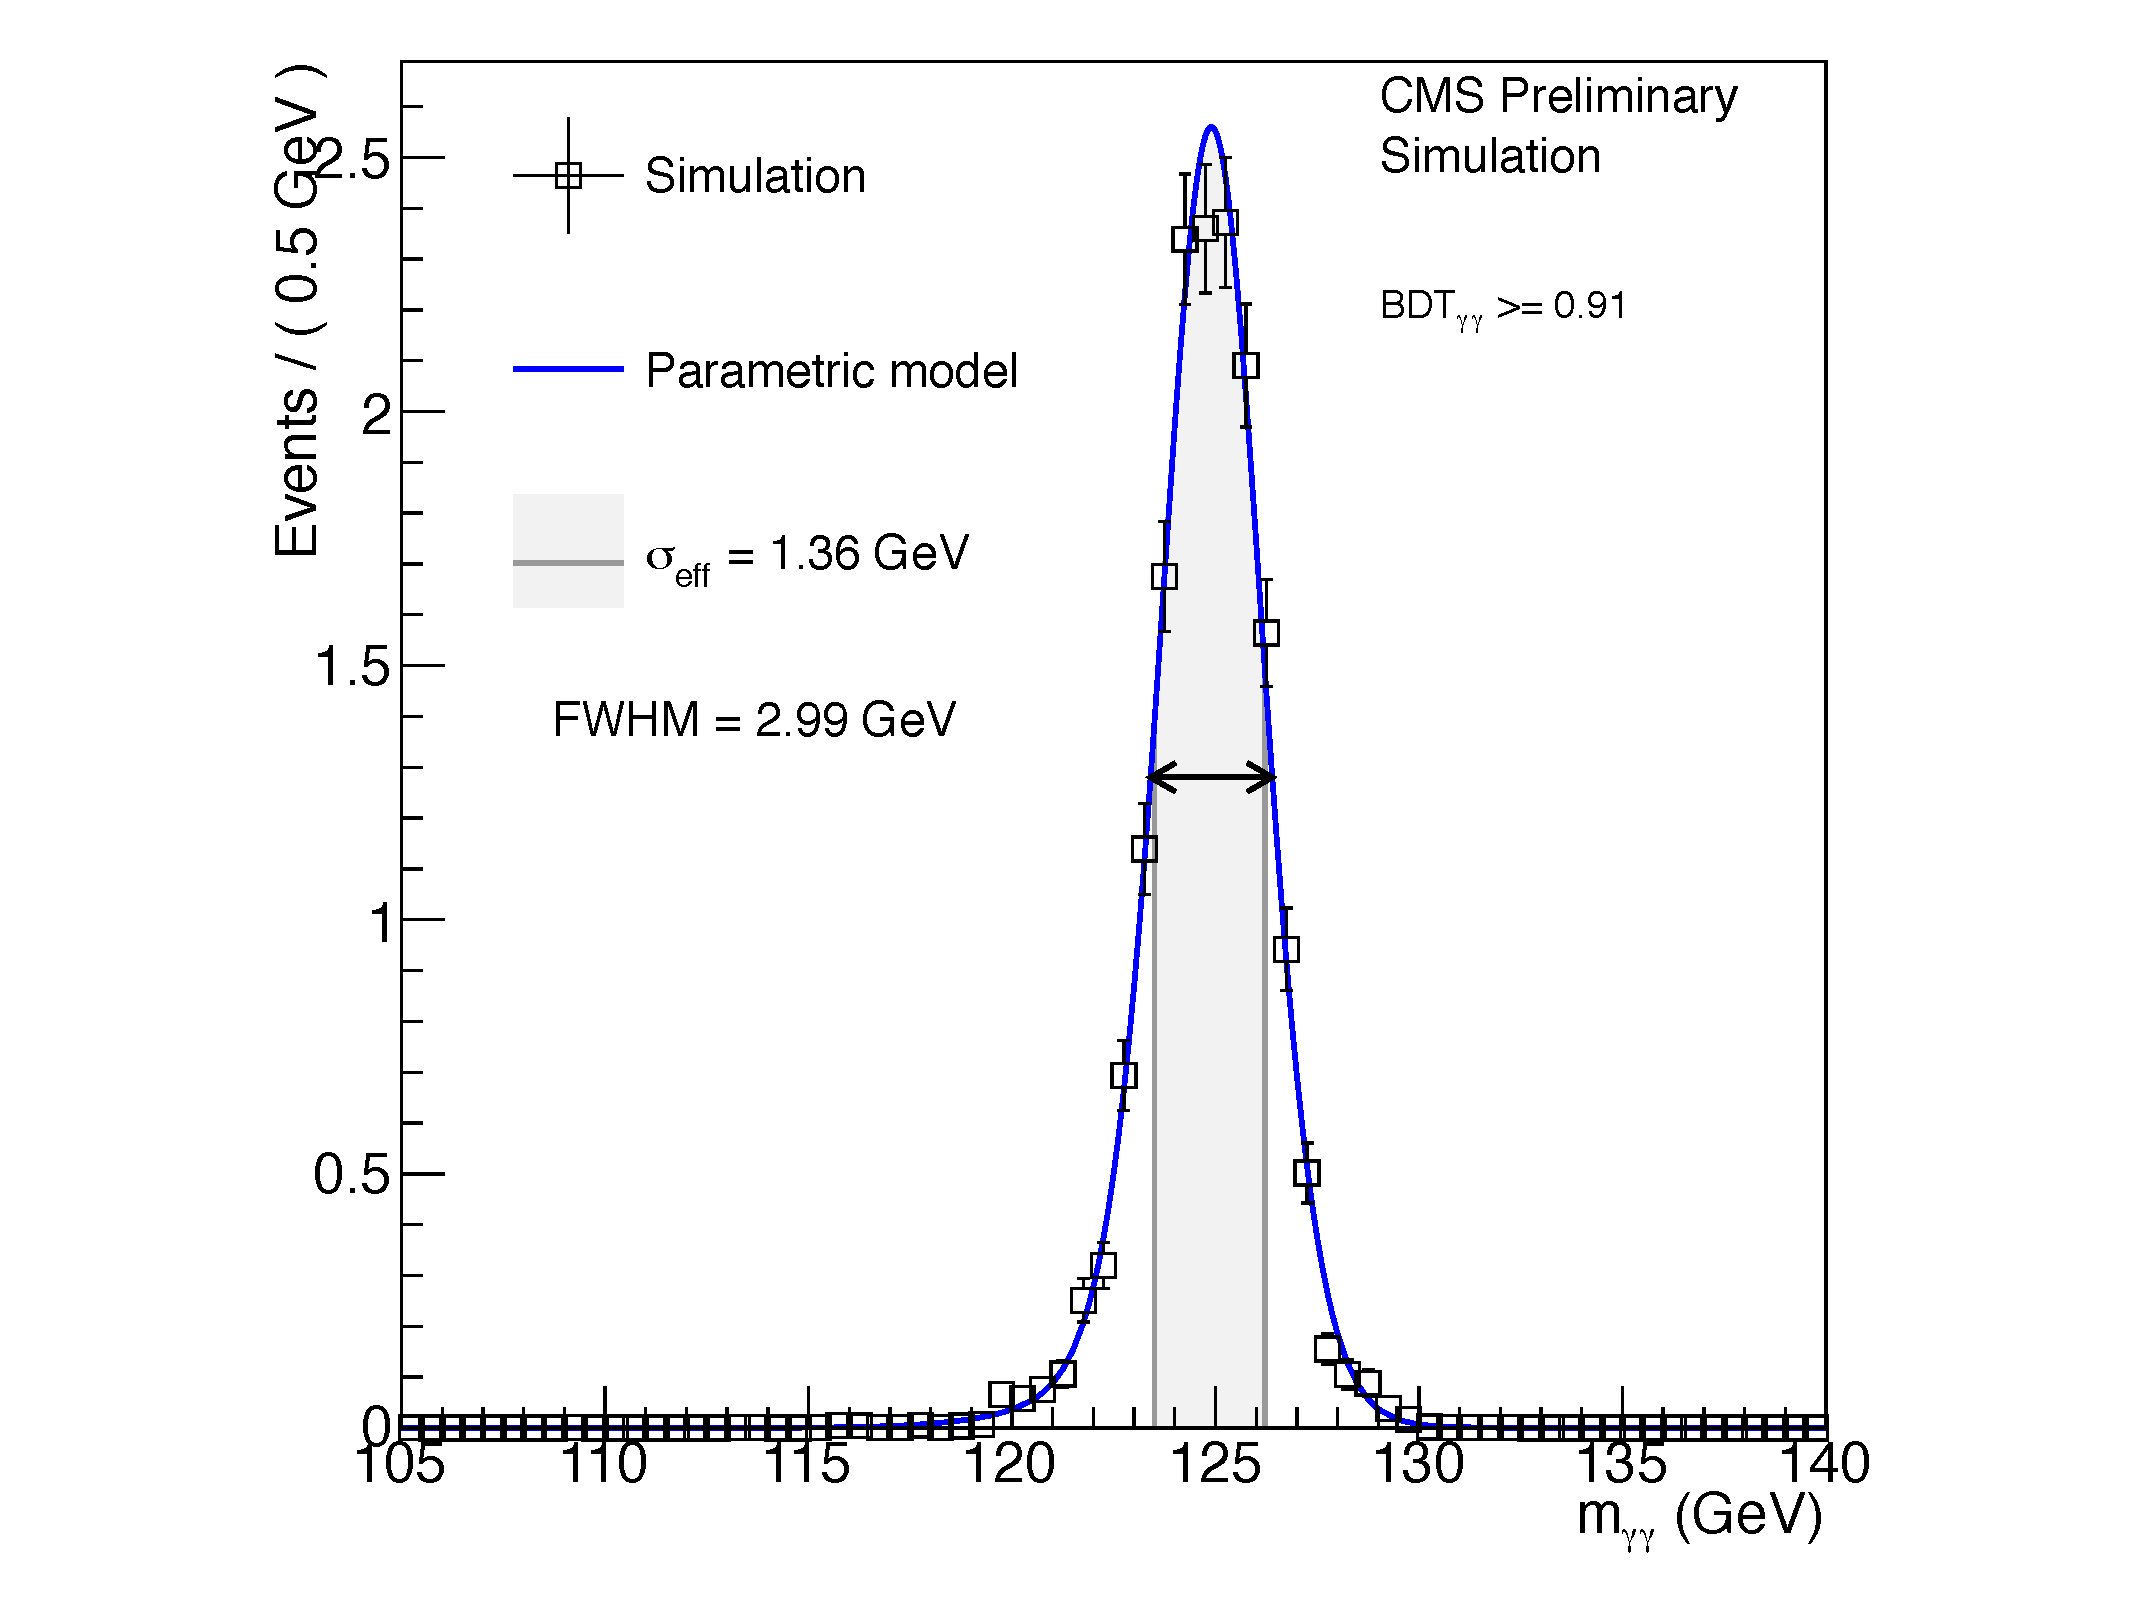
\includegraphics[width=0.38\textwidth]{CMS_DetectorFigures/ECAL_HiggsMassRes.pdf}
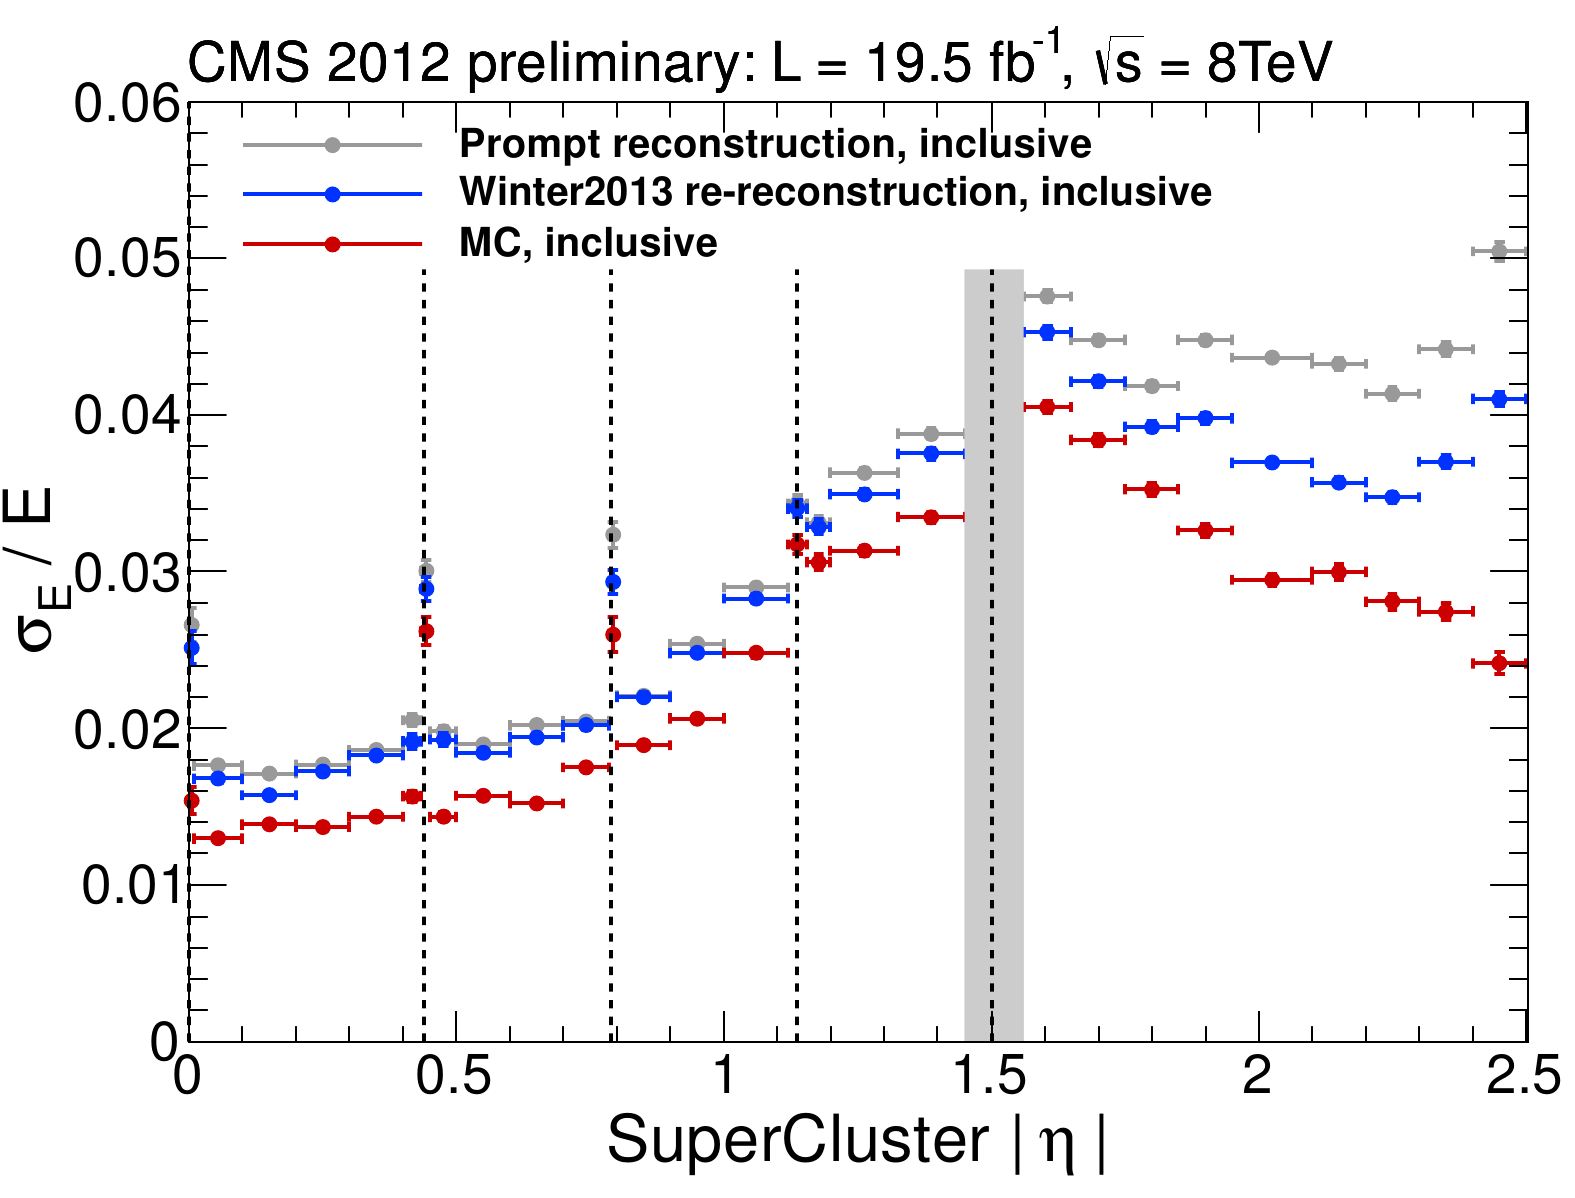
\includegraphics[width=0.49\textwidth]{CMS_DetectorFigures/EcalScaleEta_Incl.png}
\caption{The reconstructed Z invariant mass from $e^{+}e^{-}$
  decays. The left and right panels show the reconstructed invariant mass for
  the EB and EE, repectively, with different algorithms to reconstructed electron energies.\label{fig:ECAL_Higgs}}
\end{figure}
\section{The Hadronic Calorimeter}
The CMS Hadron Calorimeter (HCAL) is sorrounds the silicon tracker and
the electromagnetic calorimeter. It is composed of four different
subsytems: the barrel (HB), endcaps (HEs), the outer (HO), and the
forward (HF) calorimeters. The HB and HE are located inside the
cryostat of the superconducting solenoid and both are sampling
calorimeters with brass as the absorber and plastic scintillator as
the active meadium. The HO is plastic scintillator calorimeter located outside the superconducting
solenoid cryostat and is designed to catch the energy leakeage from
the HB. The HF is a quartz fiber and steel calorimeter located at $z
=\pm$ 11.15 m, thus, extending the pseudorapidity coverage up to
$|\eta| = 5$. The layout of the HCAL is presented in
Figure~\ref{fig:HCAL_Layout}.

\begin{figure}
 \centering
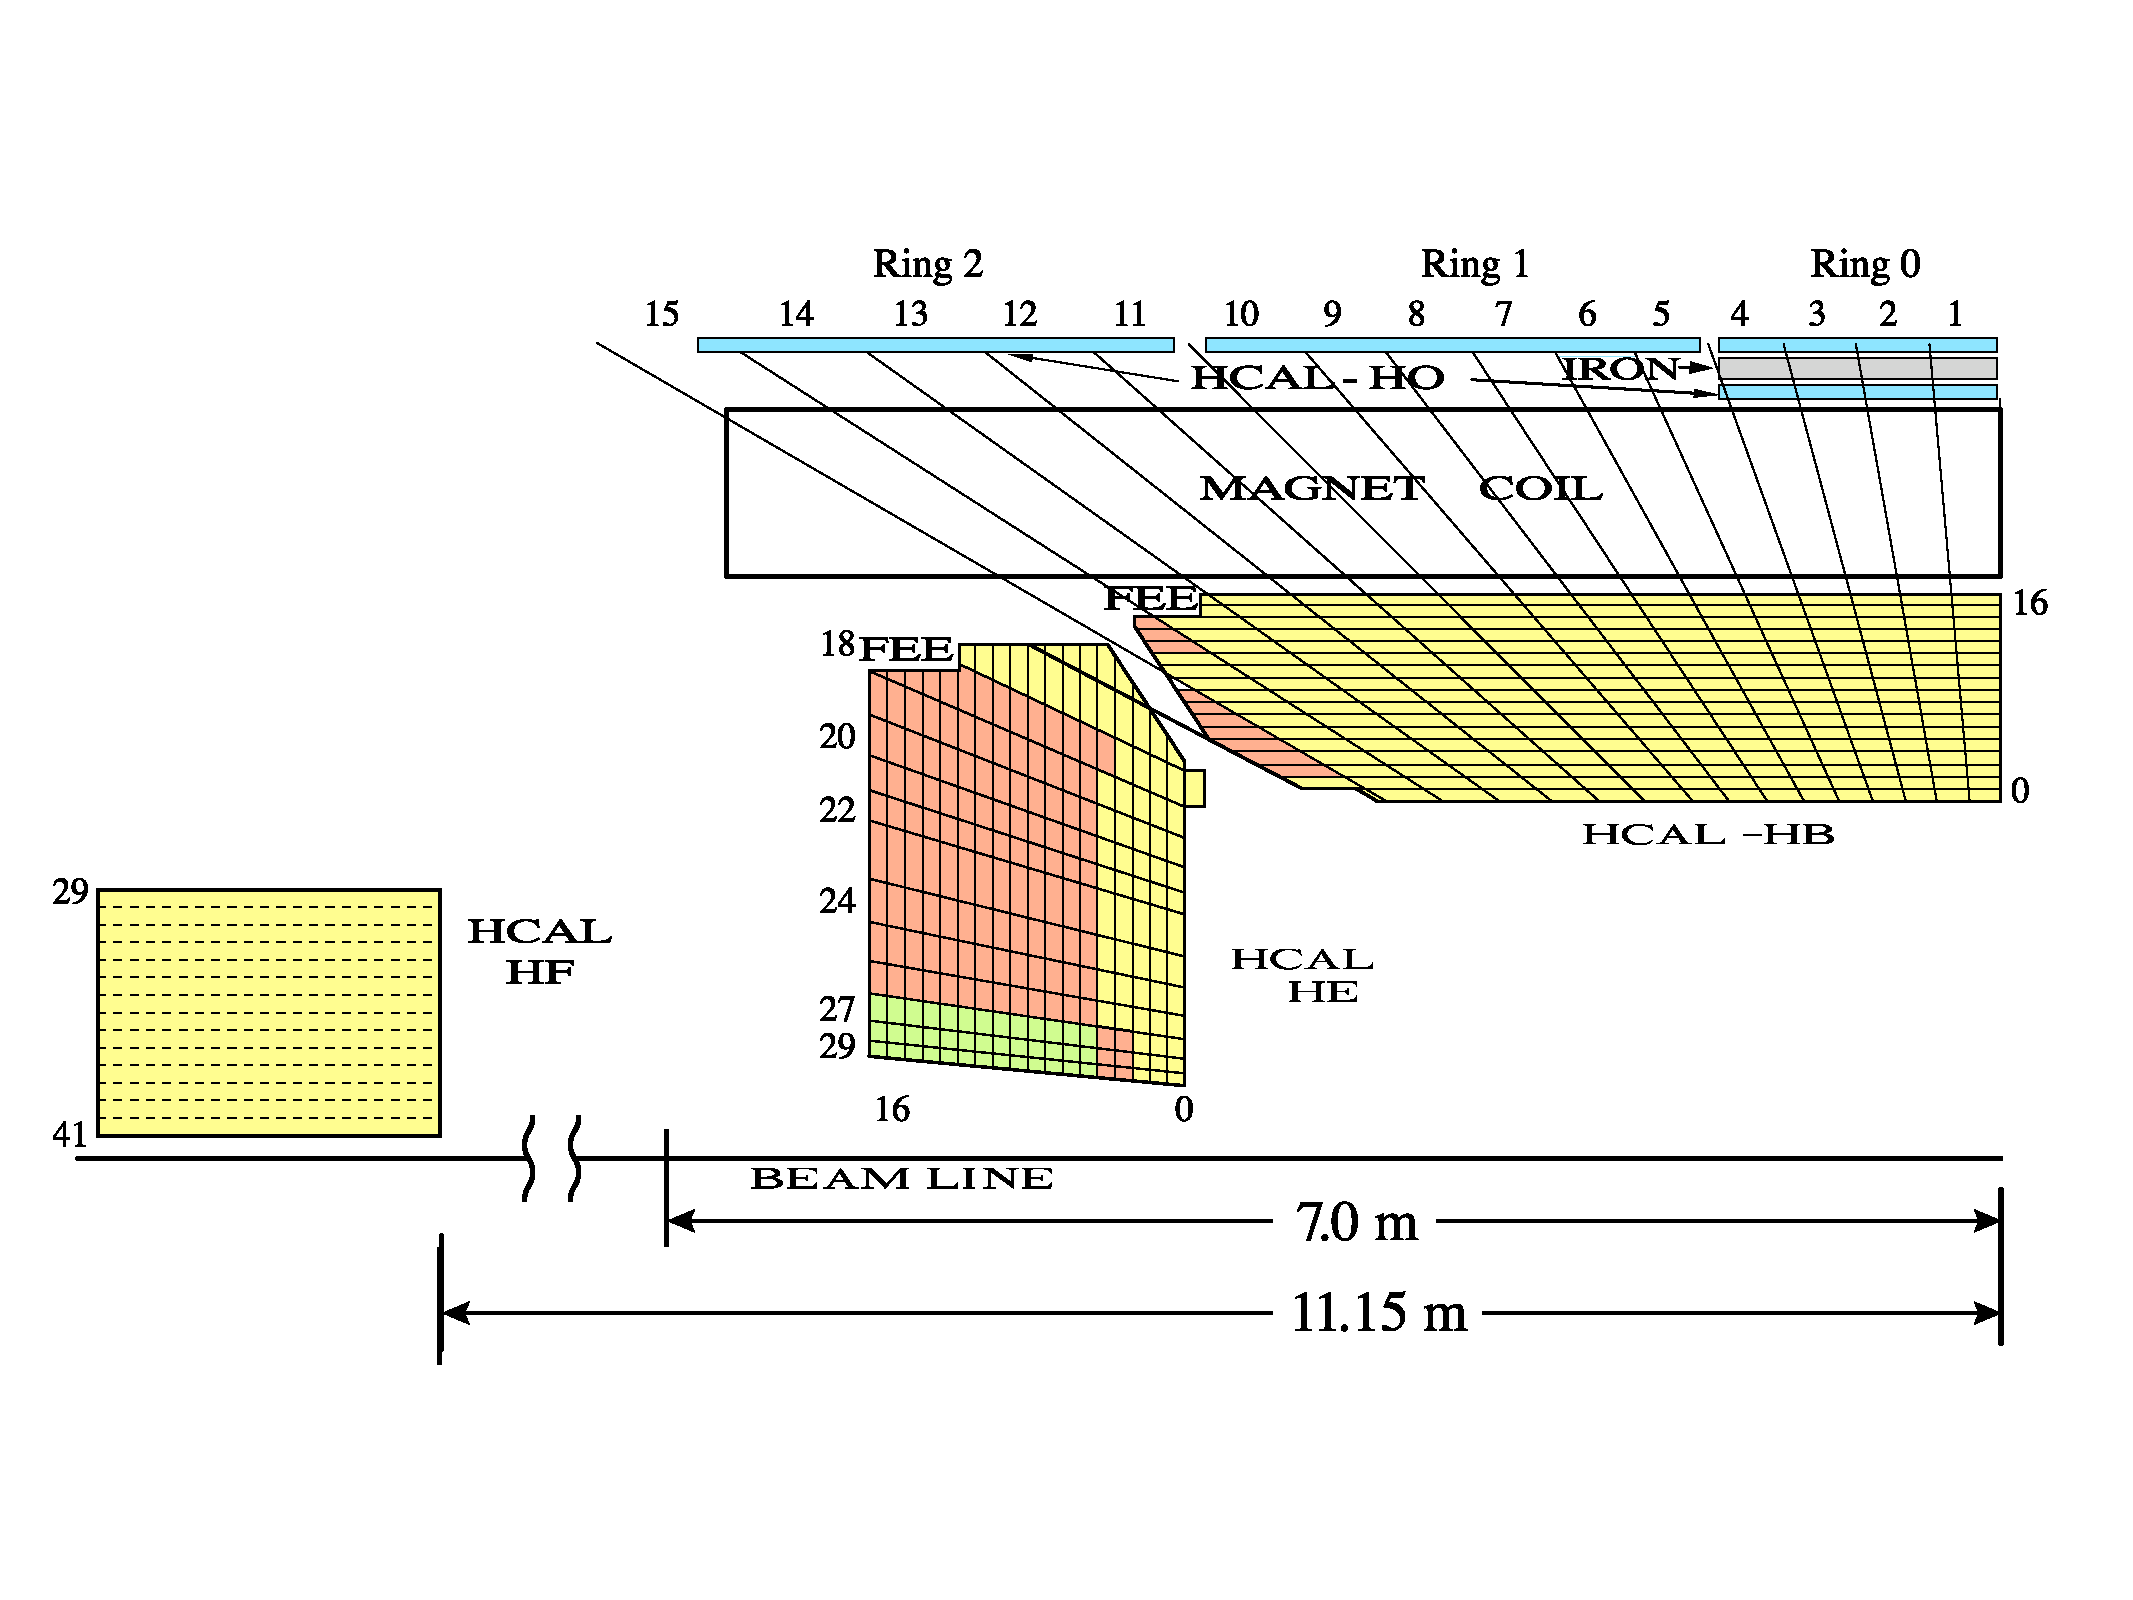
\includegraphics[width=0.99\textwidth]{CMS_DetectorFigures/HCAL_Layout.pdf}
\caption{The CMS HCAL layout.\label{fig:HCAL_Layout}}
\end{figure}

The hadronic energy resolution for the barrel HCAL and ECAL
combination was measured in beam test using pions and protons and
found to be:

\begin{equation}
\label{eq:hcal_res}
\frac{\sigma_{E}}{E} = \frac{0.847\pm0.016\GeV^{\frac{1}{2}}}{\sqrt{E
    (\GeV)}} \oplus 0.074\pm 0.008.
\end{equation}
The energy resolution in the endcaps is similar to that of the barrel.

The following passages are aimed to give a more detailed description
of the four HCAL subsystems.

\subsection{The Barrel Hadronic Calorimeter}
The HB is a sampling calorimeter made of brass absorber and plastic
scintillator as the active medium. The whole EB is build out of two
identical cylindrical structures, each of which is composed of 18
brass wedges. The pseudorapidity coverage of the HB reaches
approximately $|\eta| = 1.4$ while the $\phi$ covarage is
360$^{\circ}$. The segmentation of the HB is provided by the plastic
scintillator tiles inserted in the layers of the brass wedges, the later
are segmented into four $\phi$ sector, while there are 16 scintillator
tiles along the $\eta$ direction, thus providing the HB with an
equivalent segmentation of 0.087$\times$0.087 in $\eta$, $\phi$. Each
wedge calorimeter is composed of 16 layers of absorber and 17 layers of
plastic scintillator, the intermediate layer are made of brass
absorber and 3 mm plastic scintillator while the first and last layers
are made of stainless steel  and thicker 9 mm plastic scintillator
tiles. The very first layer is scintillator in order to detect showers
developed in the electromagnetic calorimeter
material. Figure~\ref{fig:HCALwedge} shows an schematic of a HB
wedge. The 16 scintillator tiles of each layer are laid in a tray in
order to facilitate their insertion and removal. Each tile's
scintillating light is collected by a green double-cladded
wavelength-shinting (WLS) fibers from Kuraray (Y-11) placed in groove
in the scintillator. Upon exiting the scintillating tile, each WLS is
splice into a clear fiber which subsequently ends in an optical
connector at the back of the tray. At this point, optical cables
take the light from the clear fiber into a 19 pixel hybrid photodiode
(HPD), which is designed to work inside the 3.8 T magnetic field. The
total interaction lengths ($\lambda_{I}$) of the HB varies with
pseudoparidity, there are 5.8 $\lambda_{I}$ at $\eta = 0$, increasing
up to 10.6 $\lambda_{I}$ at $|\eta| = 1.3$.
The finalized HB is shown in Figure~\ref{fig:hcal}.
\begin{figure}
 \centering
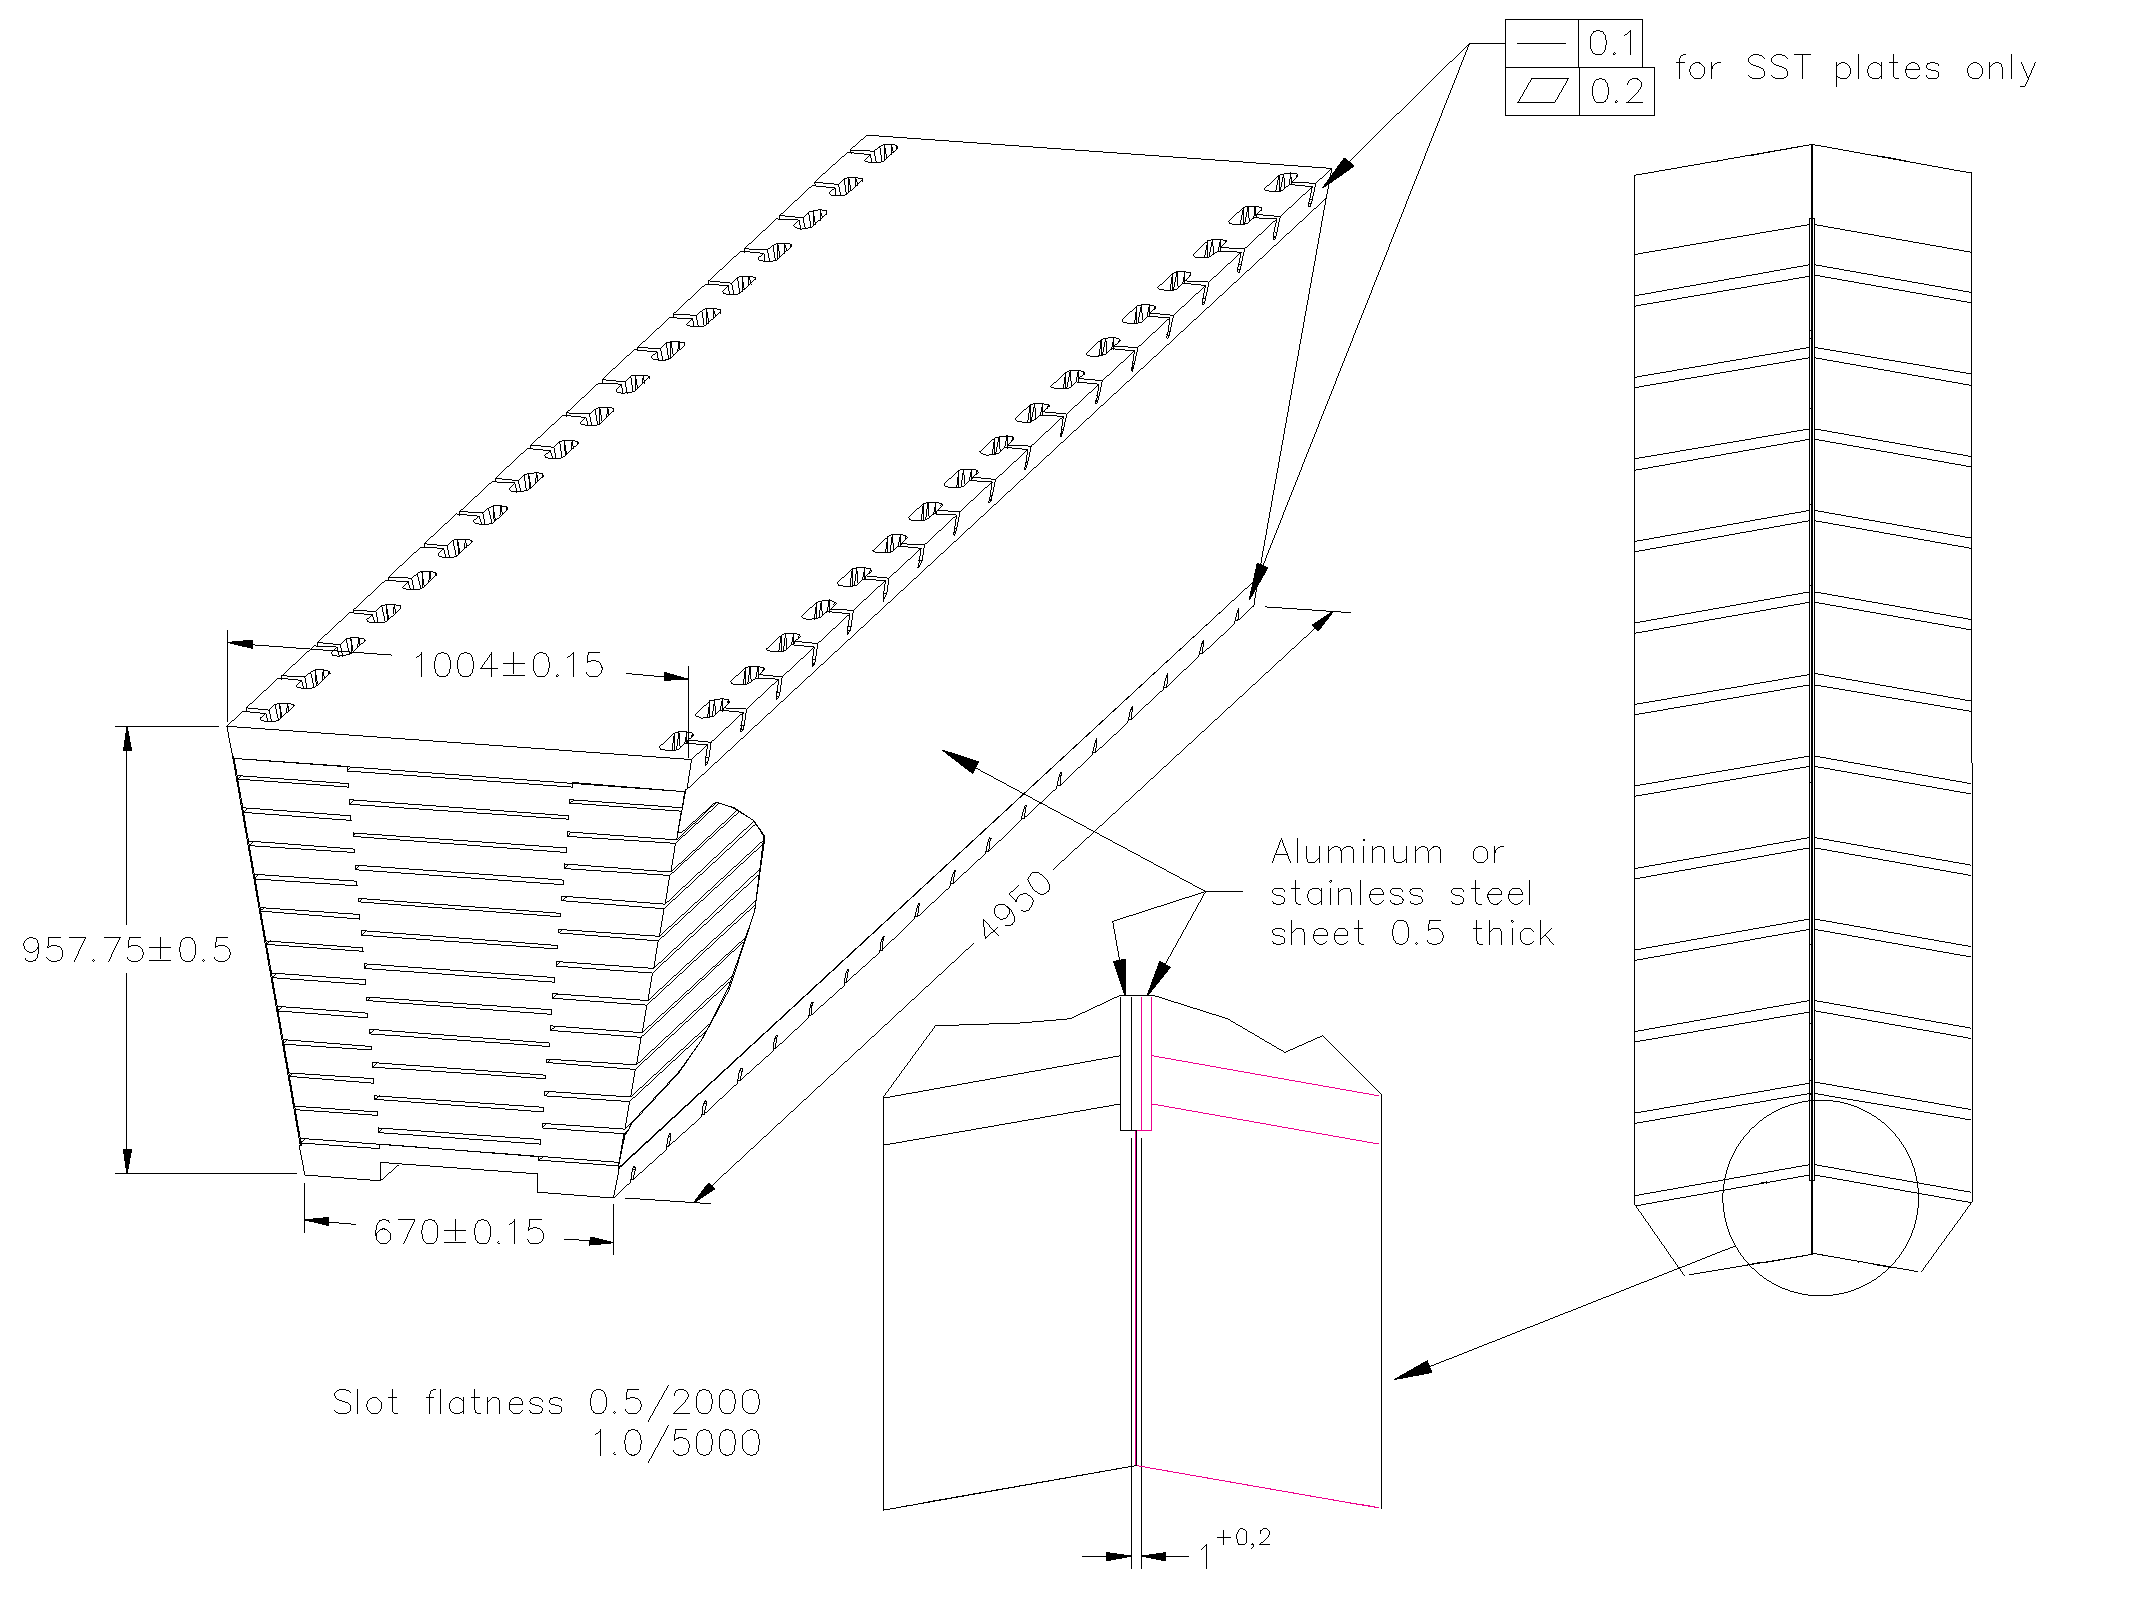
\includegraphics[width=0.99\textwidth]{CMS_DetectorFigures/HCAL_Wedge.pdf}
\caption{An schematic drawn of one of the wedges of the CMS HB.\label{fig:HCALwedge}}
\end{figure}
\begin{figure}
 \centering
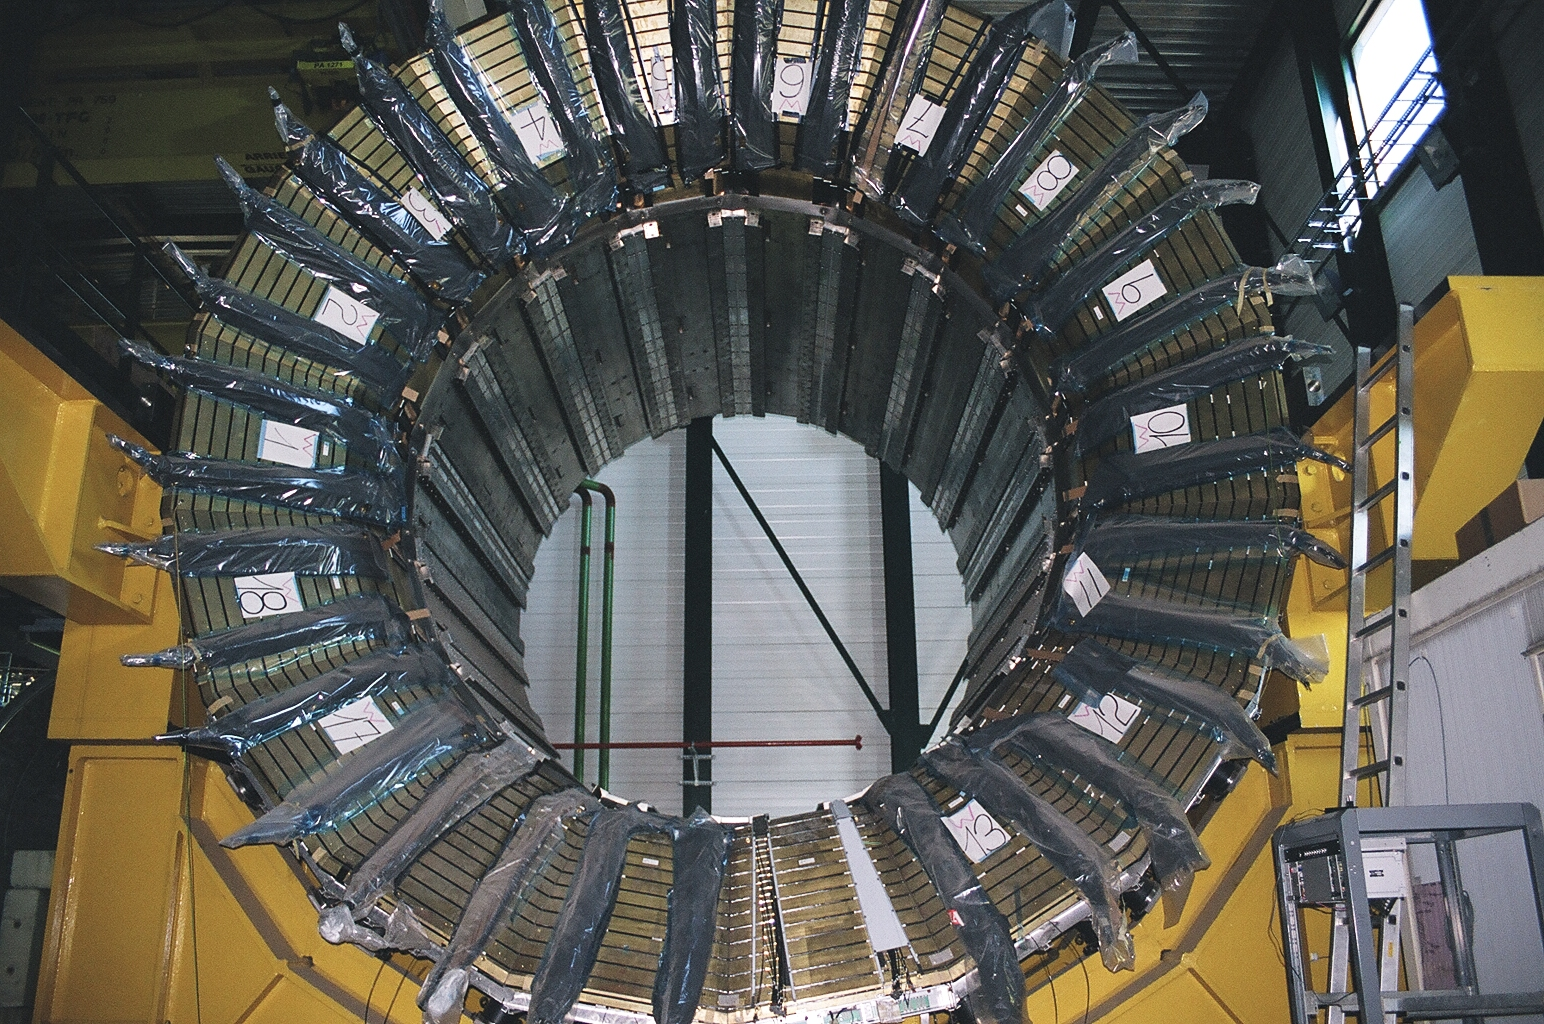
\includegraphics[width=0.99\textwidth]{CMS_DetectorFigures/hcal-HB.jpg}
\caption{A photograph of the finalized CMS HB.\label{fig:hcal}}
\end{figure}
\subsection{The Endcap Hadronic Calorimeter}
The HE is a brass/platic-scintillator sampling calorimeter that extend
the pseudorapidity coverage from $1.3 < |\eta| < 3$. It is composed of
79-mm-thick brass plates with 9 mm gaps to accomodate the
scintillator. The total material, including the crystals in the EE, is
about 10 $\lambda_{I}$. There are 18 layers -- along the $z$-direction
-- of plastic scintillators, the first layer, right after the EE, is
9-mm-thick, while the rest are 3-mm-thick. The scintillators are
segmented in the radial direction and their light is collected by
embedded WLS fiber. The scintillator tiles and the WLS are laid in
trays with a trapezoidal geometry. Figure~\ref{fig:HEtiles} shows an
schematic of the trays. The WLS are spliced to clear fibers which are
susequently terminated in an optical connector. Optical cables
transport the light from the optical connector the HPDs, which, as
mentioned earlier, could operate in the presense of a magnetic
field. This design results in a granularity of 0.087$\times$0.087
($\eta\times\phi$) for $|\eta| < 1.6$ and 0.17$\times$0.17 for $|\eta|
> 1.6$. Figure~\ref{fig:HE} shows one partially finalized HE, where
only some of the scintillator trays have been inserted.

\begin{figure}
 \centering
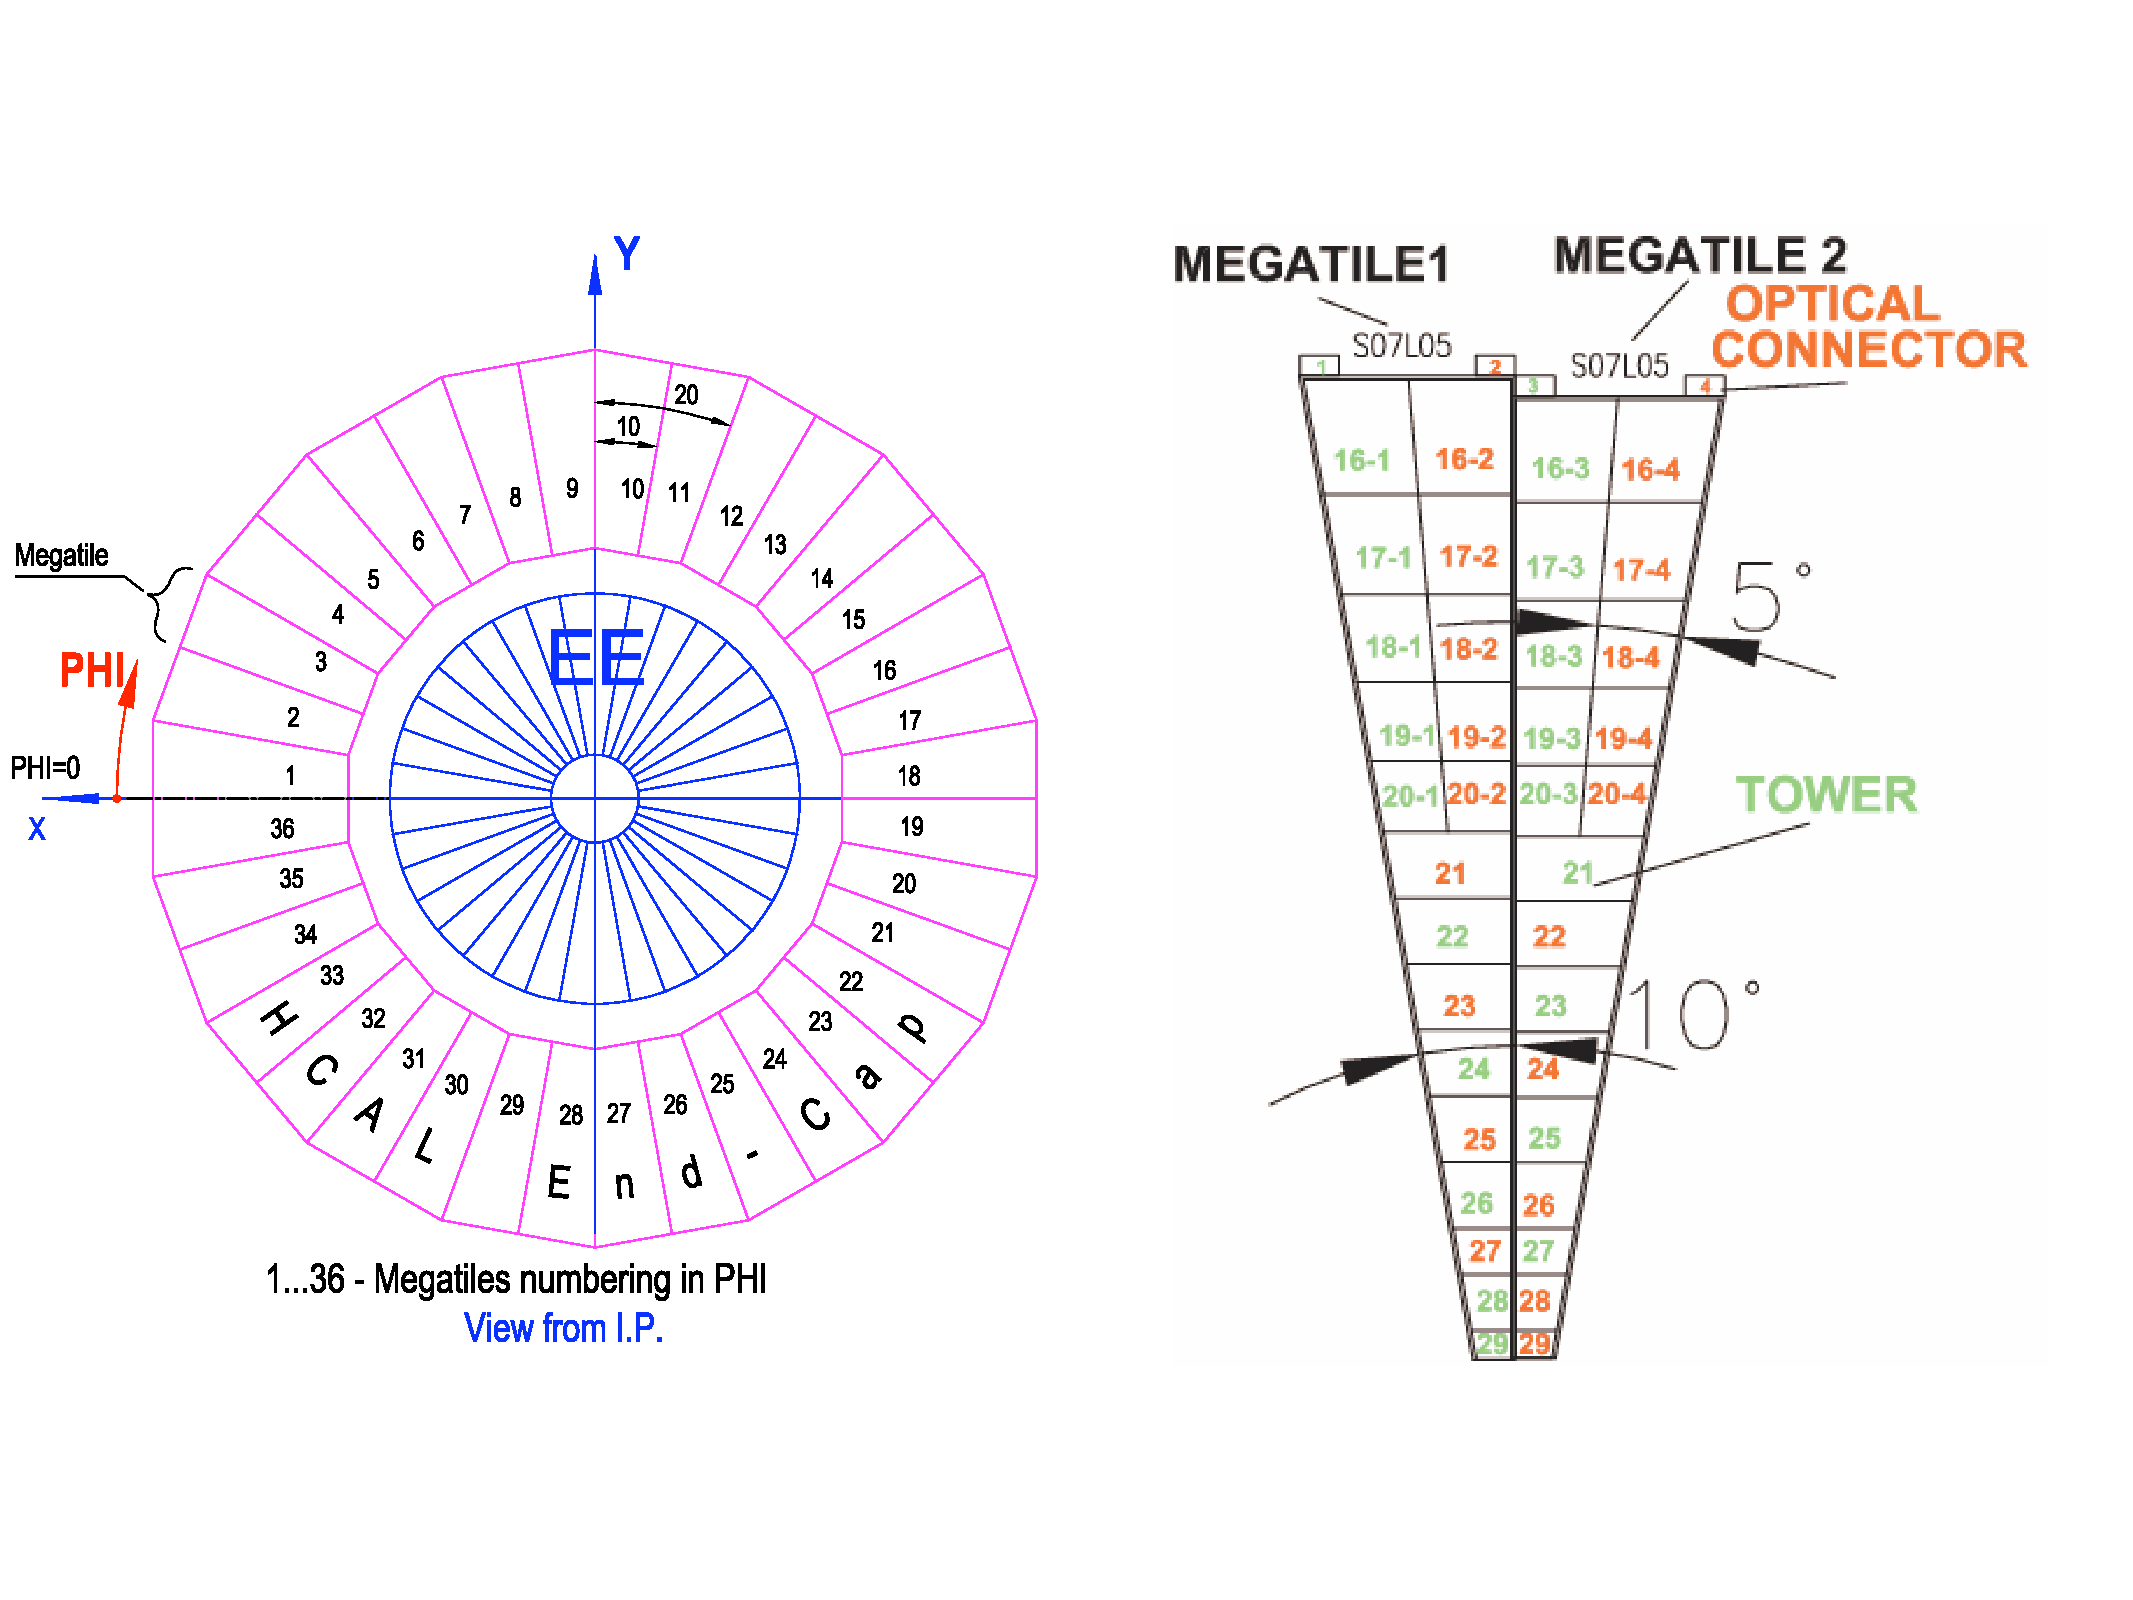
\includegraphics[width=0.99\textwidth]{CMS_DetectorFigures/hca_tile.pdf}
\caption{An schematic of the HE geometry in the $\phi$ direction is
  presented in the left panel. The configuration of two adjacent
  scintillator trays is presented in the right panel.\label{fig:HEtiles}}
\end{figure}
\begin{figure}
 \centering
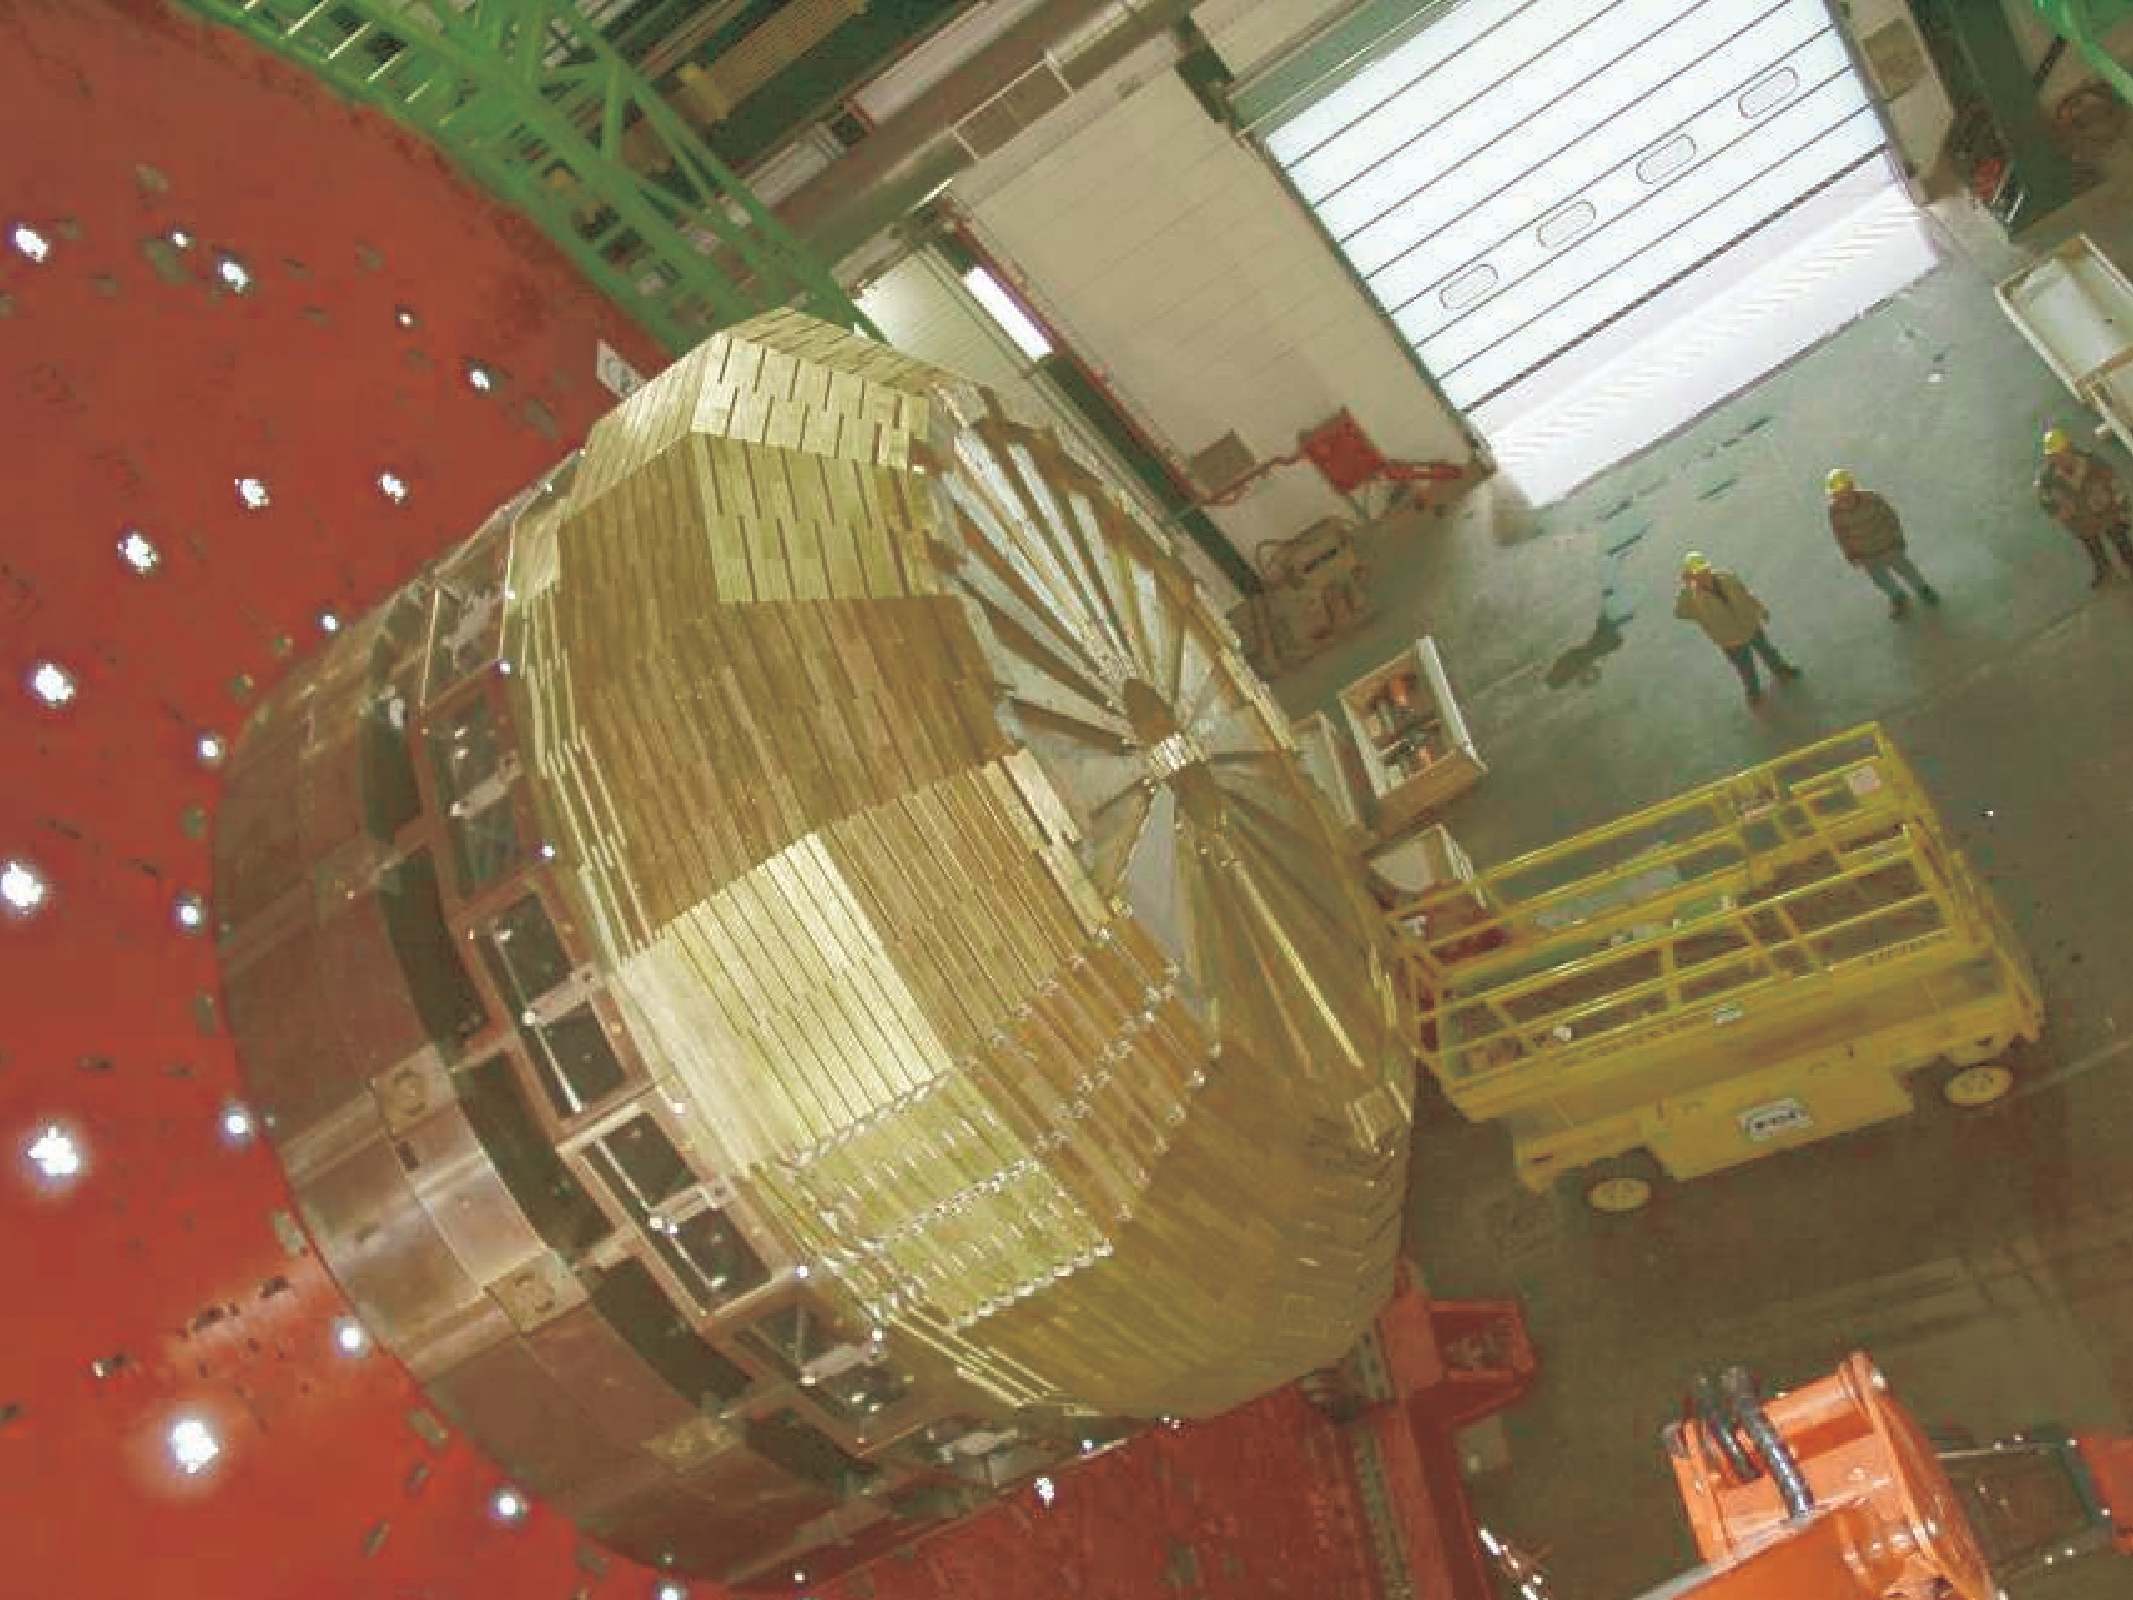
\includegraphics[width=0.99\textwidth]{CMS_DetectorFigures/hcal_HE.pdf}
\caption{A photograph of the one partially finalized CMS HE.\label{fig:HE}}
\end{figure}

\subsection{The Outer Hadronic Calorimeter}
The space constraints posed by the superconducting solenoid limited
the stopping power of the combined EB and HB and therefore their
ability to fully contain hadronic showers. In order to overcome this
limitation, another calorimeter layer, the HO, is located just outside the
cryostat of the superconducting solenoid in the central region
($|\eta| < 1.3$) of the detector. The HO uses the solenoid coil as an
additional absorber layer equivalent to 1.4/sin($\theta$)
$\lambda_{I}$. The active layer are 10-cm-thick plastic
scintillator. The geometry of the HO is constraint to that of the
muons system and therefore is composed of 5 rings along the
$z$-direction (each ring is about 2.52 m). The HO rings are label with
number -2, -1, 0, 1, and 2 which are located at $z$-positions of
-5.342 m, -2.686 m, 0, +2.686 m, and +5.342 m, respectively. The
central ring (ring-0) has two 10 cm thick layers of plastic
scintillator at each side of a 19.5 cm iron slab located $r =$ 3.82 m
and  $r =$ 4.07 m. The rest of the rings contain only one 10 cm thick
scintillator layer and no extra absorber. This brings the total
calorimeter depth to a minium of about 12 $\lambda_{I}$ except at the
boundary between the HB and the HE. Each ring is divided into 12
identical $\phi$-sectors, additionally, each sector has six scintillating tiles in
the $\phi$ direction. The two layers in ring-0 have 8 tiles the $\eta$ direction, rings 1
and -1 have have 6 tiles, and rings 2 and -2 have 6 tiles. This design
provides a granularity of 0.087$\times$0.087 in $\eta\times\phi$, thus
matching the granularity of the HB. The light from the scintillating
tiles is transported by embedded WLS which are subsequently spliced
into clear fiber -- which have a $\sim$4 time longer attenuation
length-- that finally transport the light into a photodetector outside
the muon rings. Figure~\ref{fig:HO_tile} shows the photograph of one
of the HO tiles with the embedded WLS. Finally, the geometry of the HO
is presented in Figure~\ref{fig:HO_Geometry}

\begin{figure}
 \centering
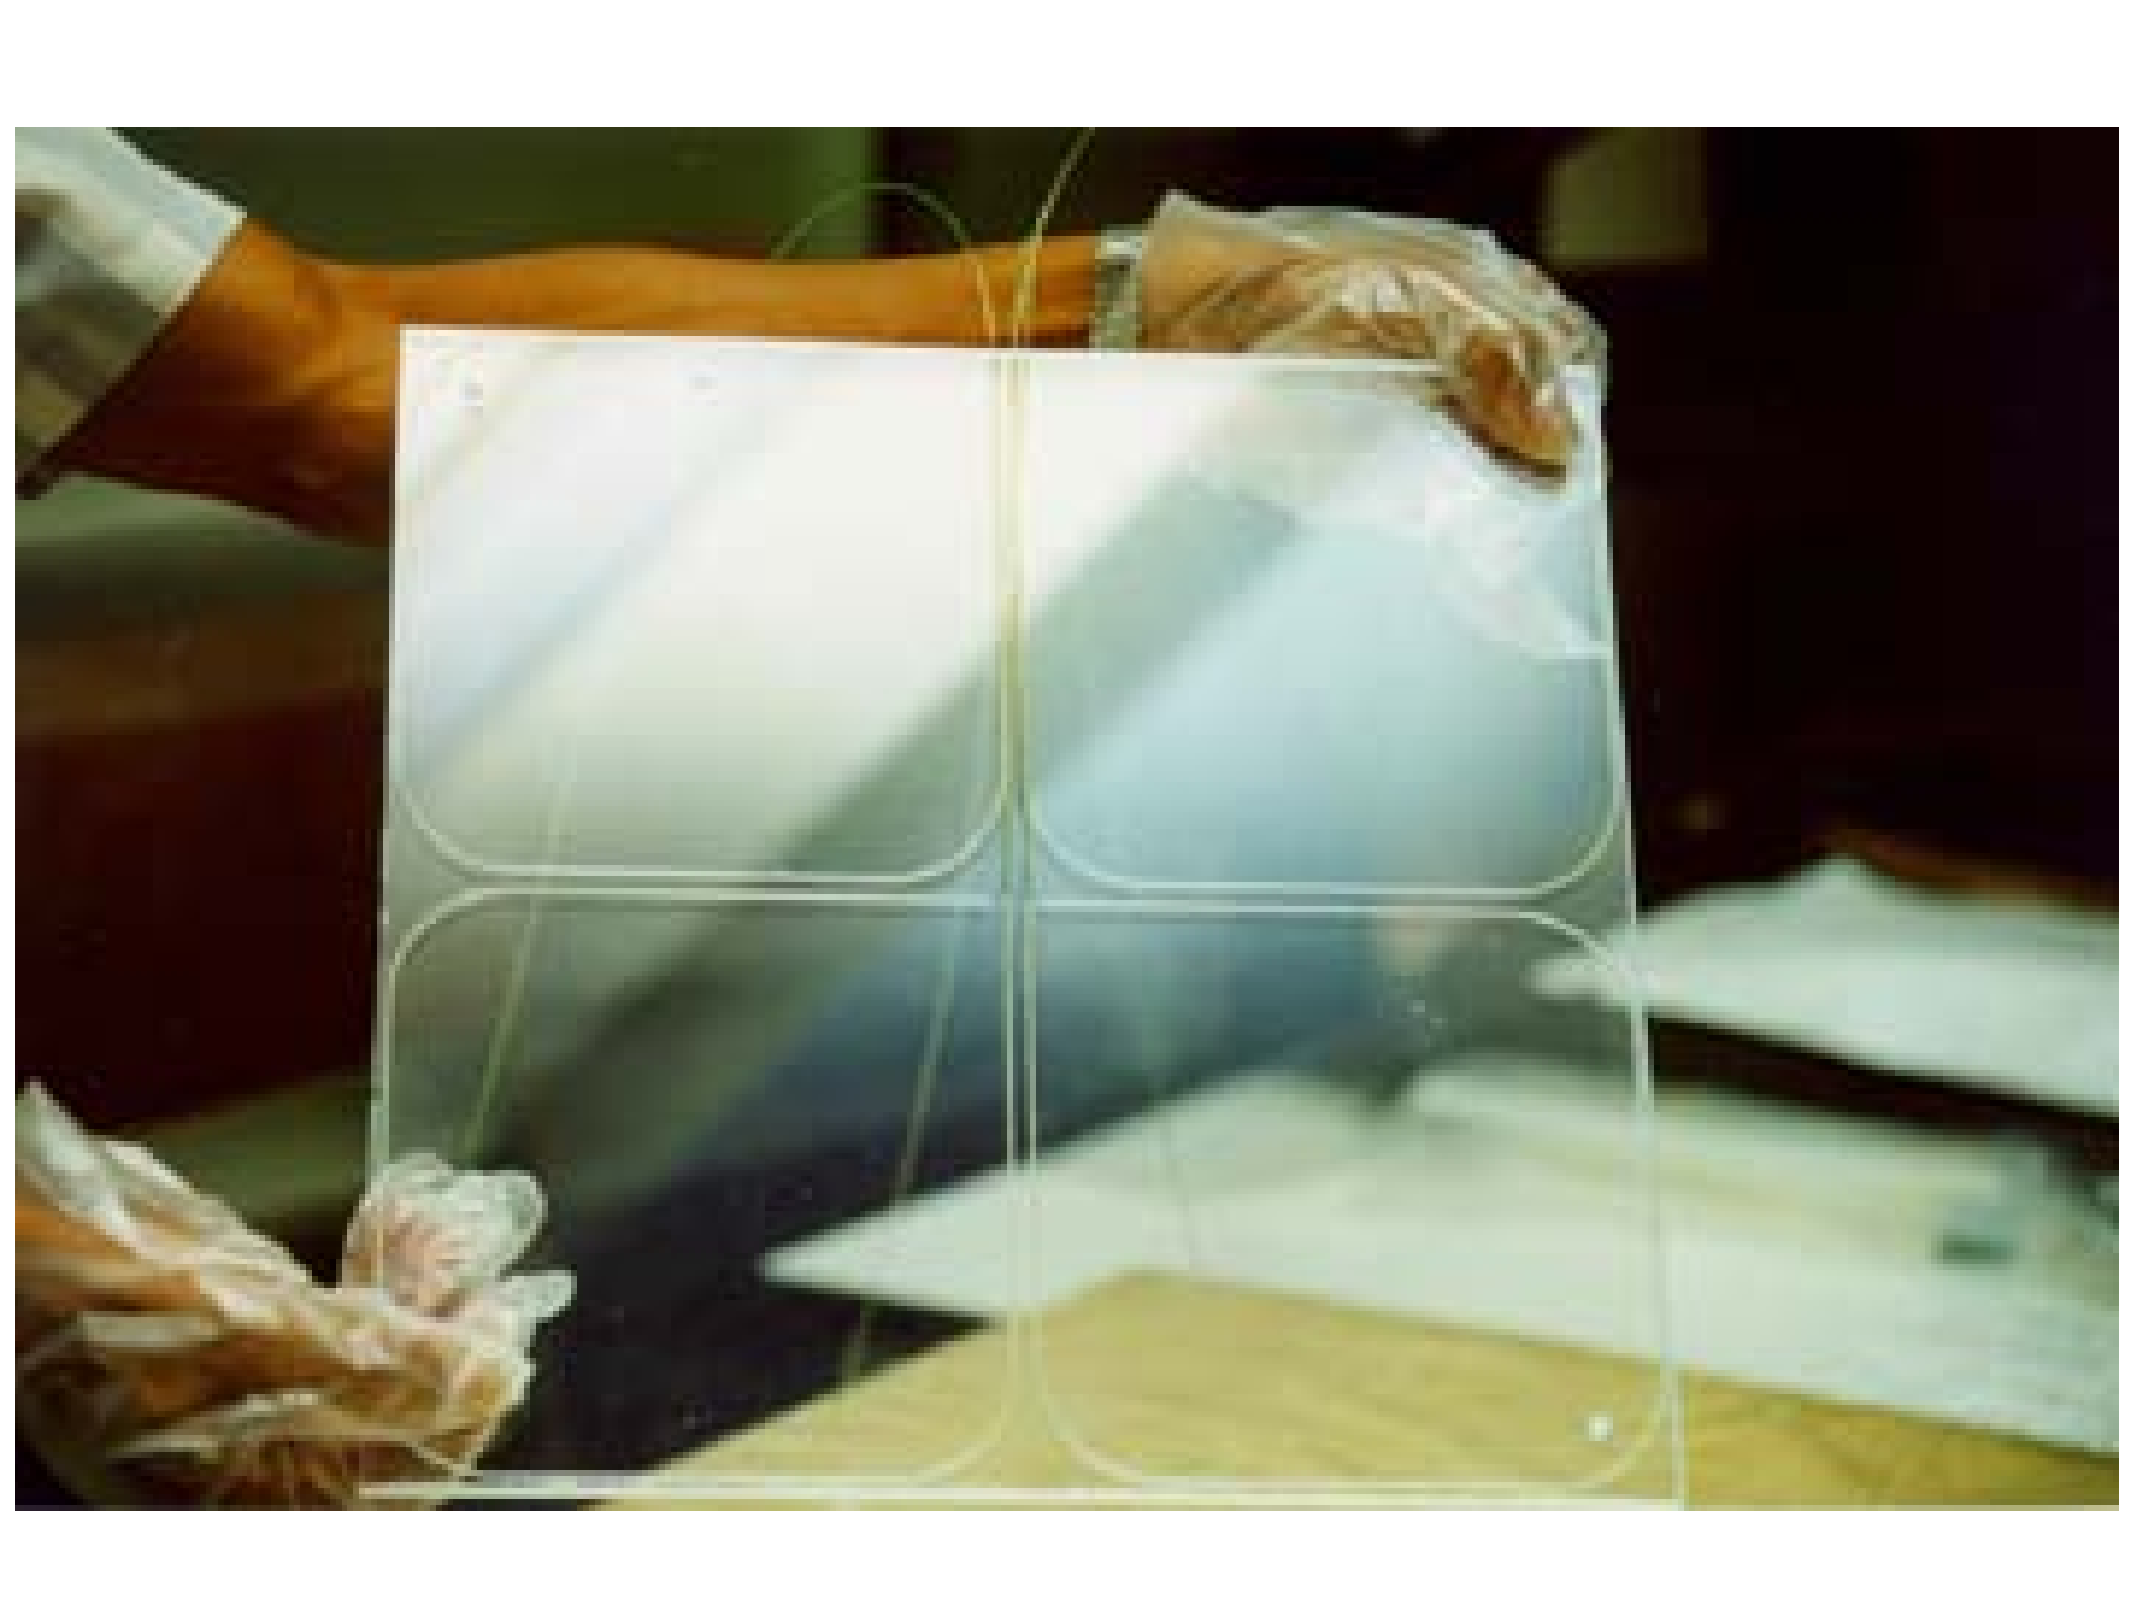
\includegraphics[width=0.6\textwidth]{CMS_DetectorFigures/HO_tile.pdf}
\caption{A photograph of a HO scintillating tile with the embedded WLS.\label{fig:HO_tile}}
\end{figure}
\begin{figure}
 \centering
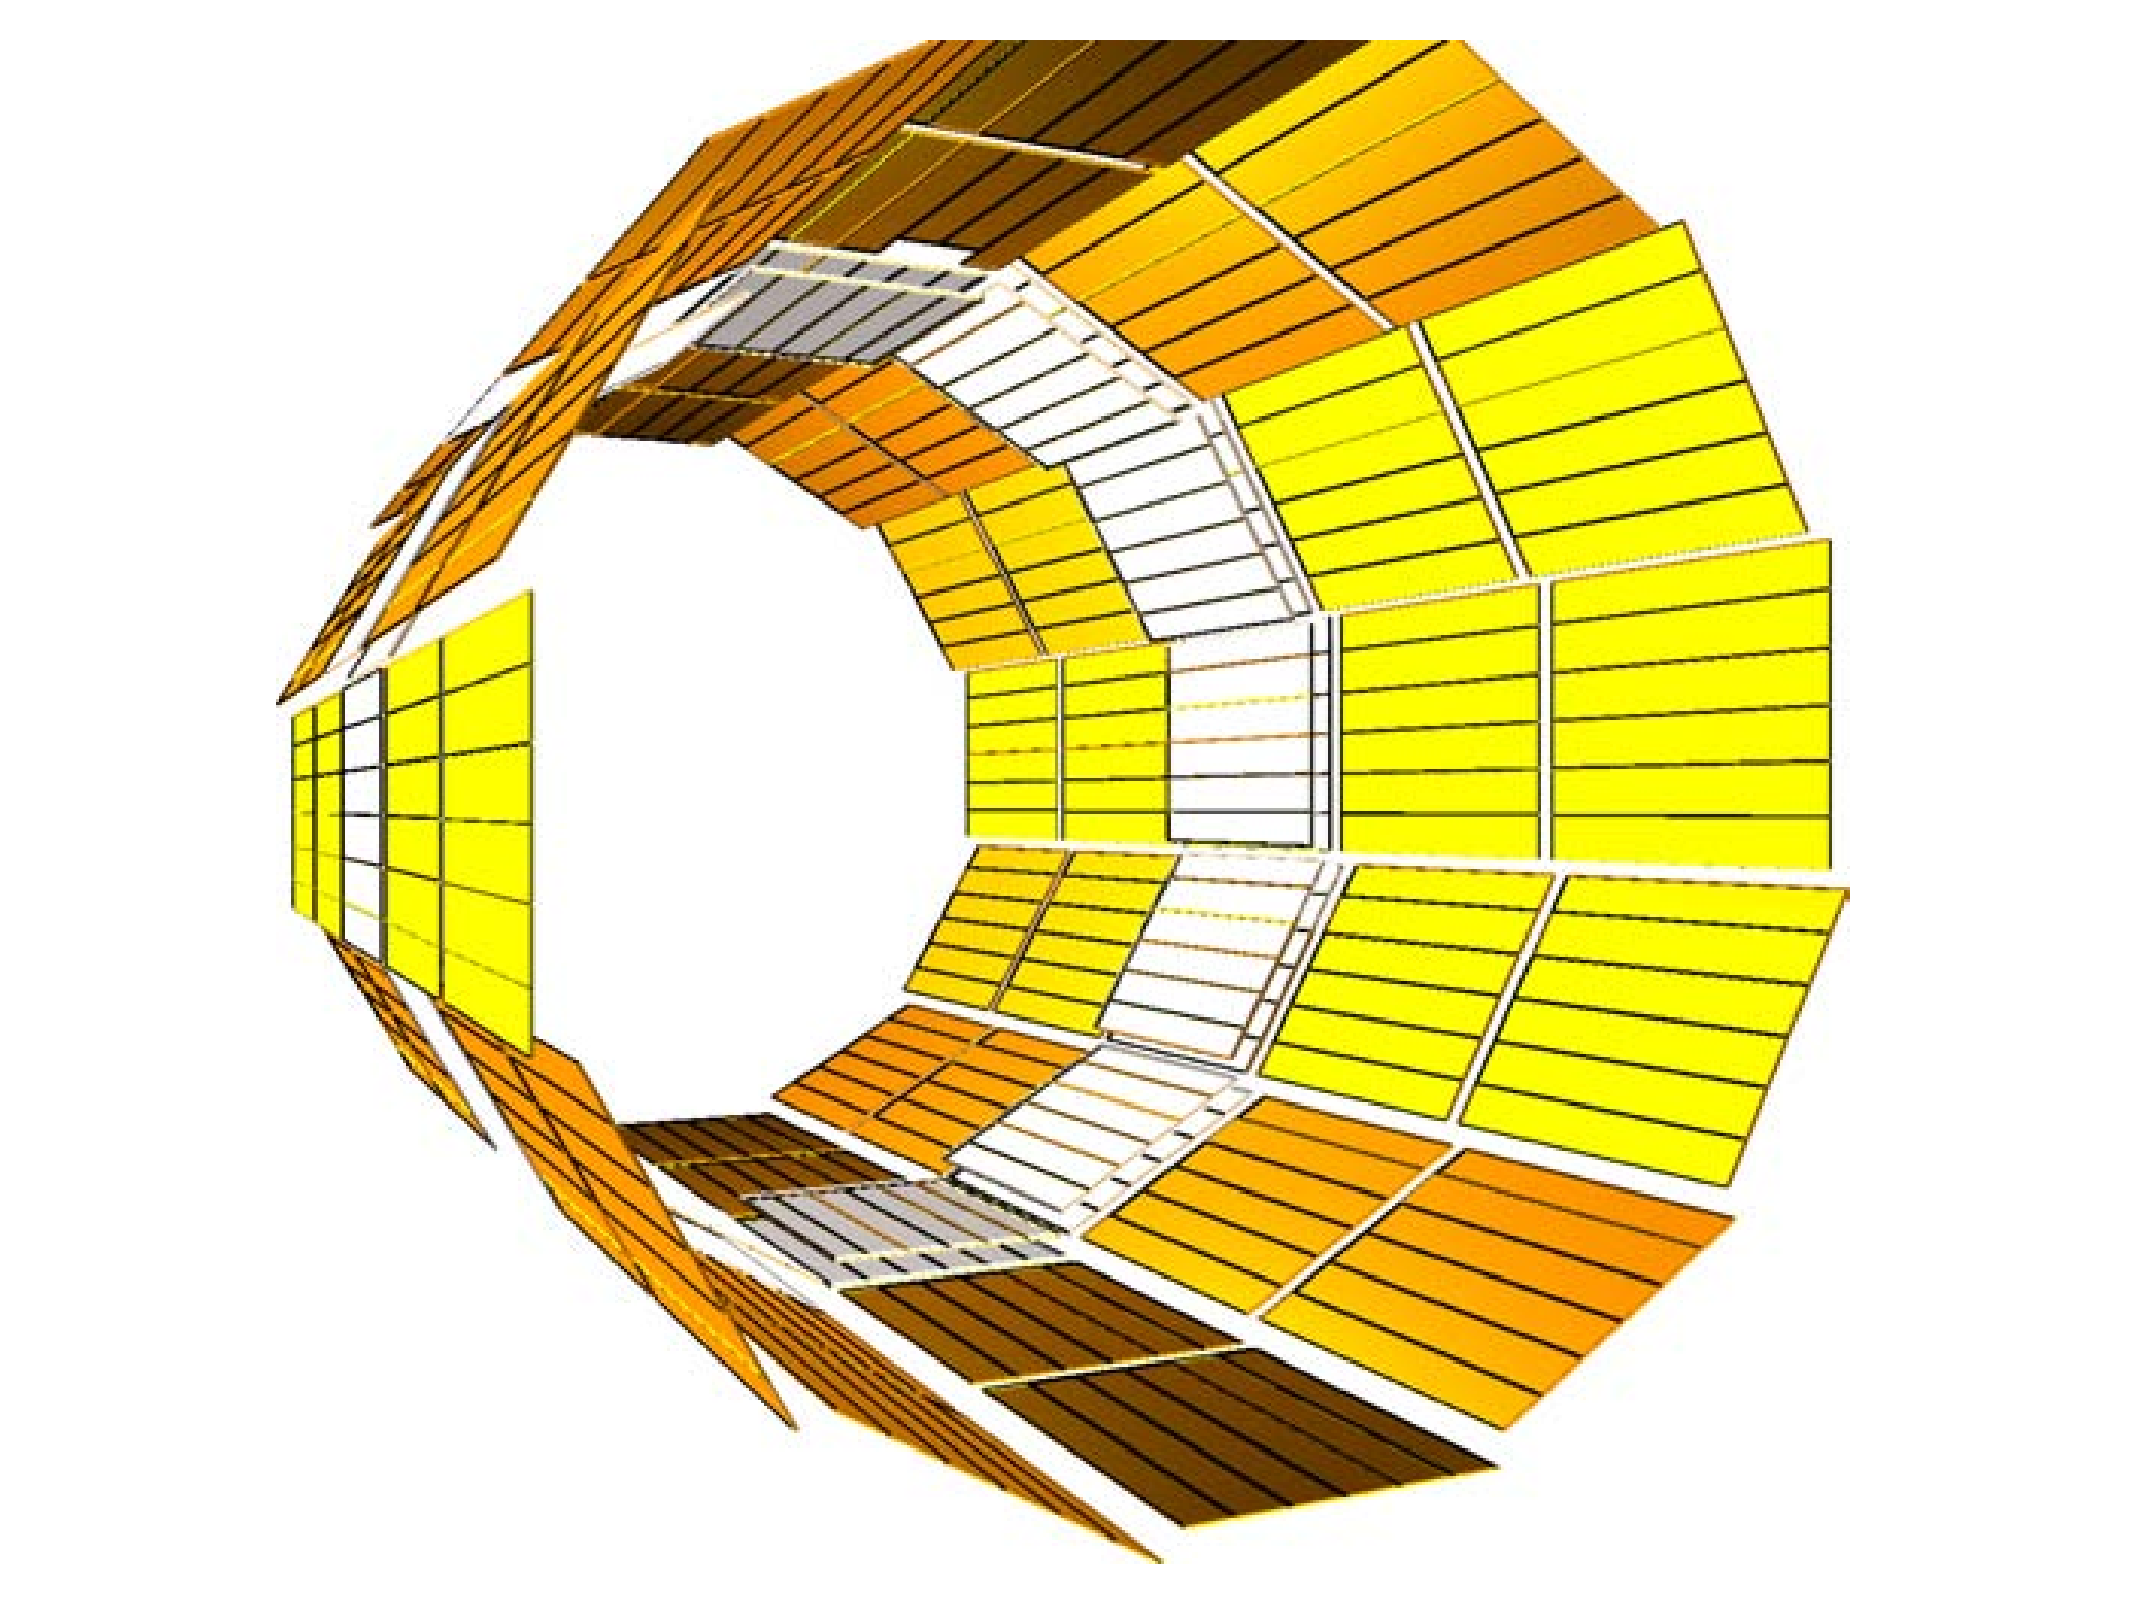
\includegraphics[width=0.6\textwidth]{CMS_DetectorFigures/HO_Geometry.pdf}
\caption{An schematic drawing presenting the geometry of the HO.\label{fig:HO_Geometry}}
\end{figure}

\subsection{The Forward Hadronic Calorimeter}
The HF cover the forward region, $3 < |\eta| 5.2$, thus receiving a
substantial amount of radiation. This harsh radiation environment was
the principal reason to use quartz fibers, due to its radiation
hardness properties, as the active medium of a
sampling calorimeter with steel absorber. The HF is a cylindrical
structure --with inner and outer radii of 12.5 cm and 130 cm, repectively -- composed of 18
steel wedges that are divided into two sectors, each wedge has quartz
fiber embedded along the $z$-direction. The quartz fibers propagate
the Cherenkov light that the secondary particle of a shower produce
when traversing through them. In order to separate electromagnetic
showers, that tend to be produced closer to the front face of the HF,
from hadronic showers; two different types of fiber are embedded in
the steel, half of the fibers cover the whole length of the HF (165 cm
$\approx 10\lambda_{I}$ ) while the other half start to run 22 cm from
the front face of the HF, these two groups are read out
separately by PMTs with a borosilicate glass window. The fiber are grouped in such a way that the effective
granularity of the HF is 0.175$\times$0.175 in
$\eta\times\phi$. Figure~\ref{fig:HF_photo} shows a photograph of some
of the HF steel wedges equipped with quartz fibers.
\begin{figure}
 \centering
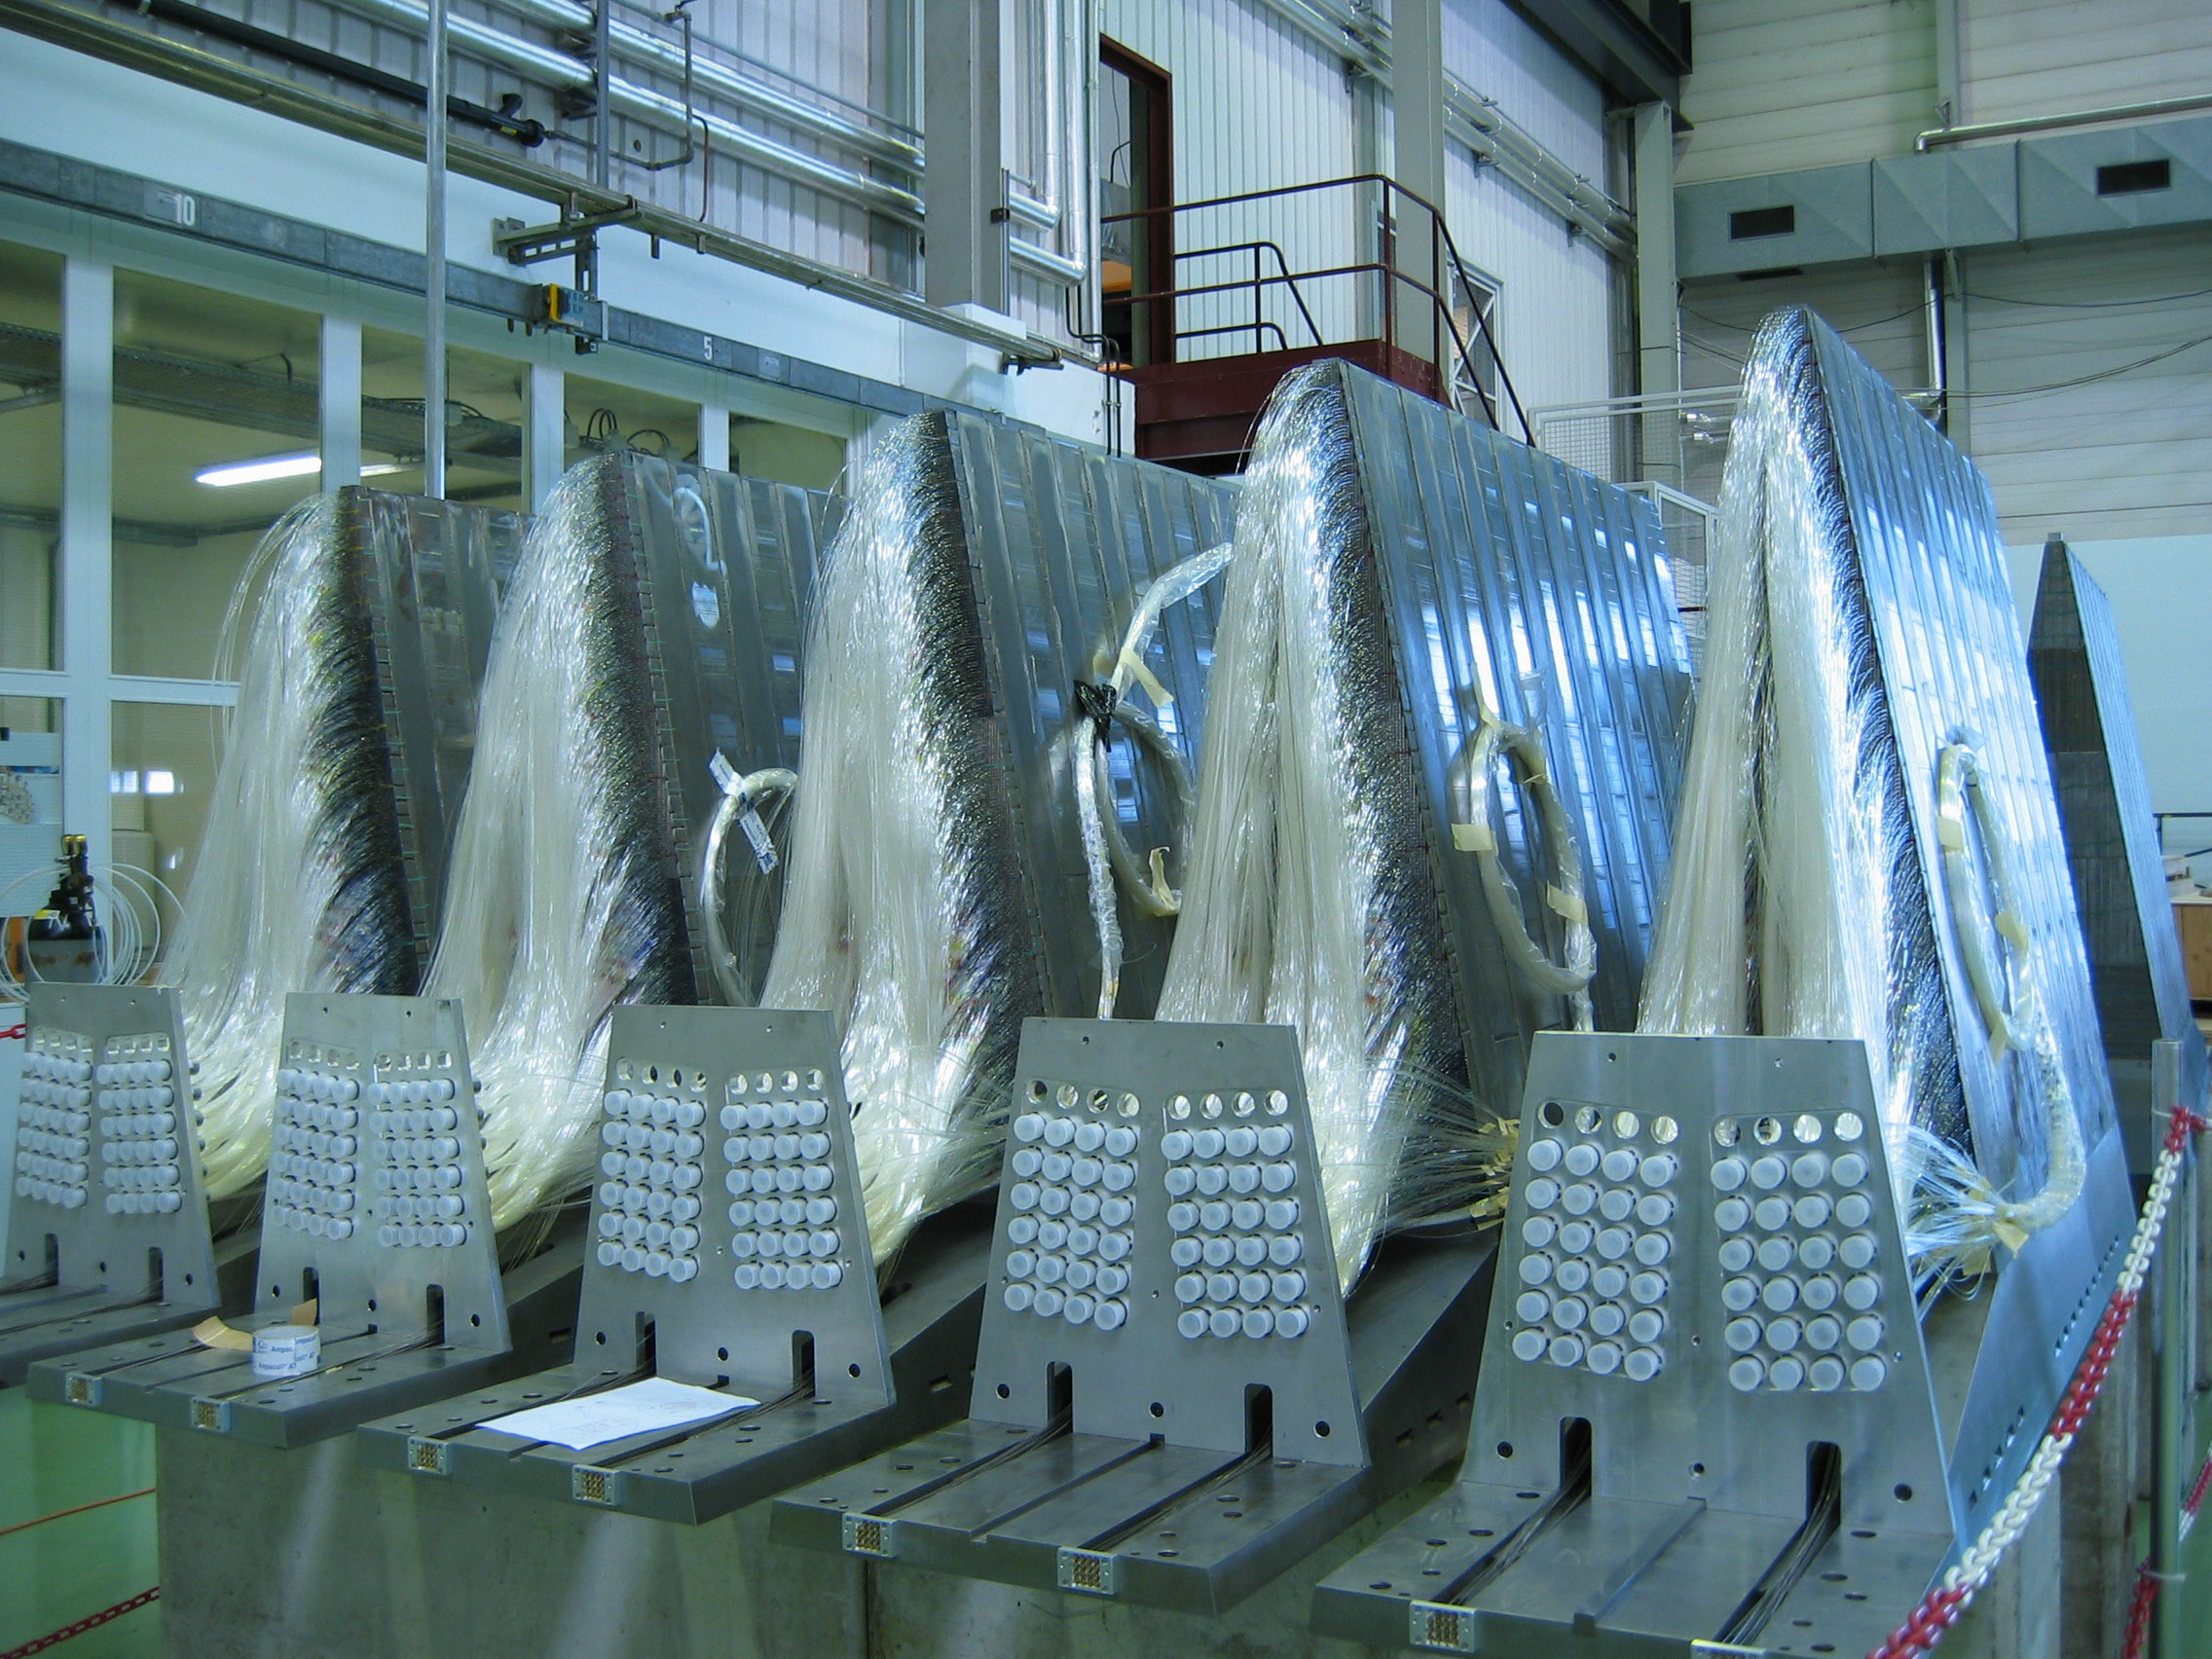
\includegraphics[width=0.7\textwidth]{CMS_DetectorFigures/HF_cal.jpg}
\caption{A photograph of the HF steel wedges equipped with quartz fibers.\label{fig:HF_photo}}
\end{figure}

\section{The Superconducting Solenoid}
\section{The Muon Chambers}